\documentclass[twoside]{book}

% Packages required by doxygen
\usepackage{calc}
\usepackage{doxygen}
\usepackage{graphicx}
\usepackage[utf8]{inputenc}
\usepackage{makeidx}
\usepackage{multicol}
\usepackage{multirow}
\usepackage{textcomp}
\usepackage[table]{xcolor}

% NLS support packages
\usepackage[french]{babel}

% Font selection
\usepackage[T1]{fontenc}
\usepackage{mathptmx}
\usepackage[scaled=.90]{helvet}
\usepackage{courier}
\usepackage{amssymb}
\usepackage{sectsty}
\renewcommand{\familydefault}{\sfdefault}
\allsectionsfont{%
  \fontseries{bc}\selectfont%
  \color{darkgray}%
}
\renewcommand{\DoxyLabelFont}{%
  \fontseries{bc}\selectfont%
  \color{darkgray}%
}

% Page & text layout
\usepackage{geometry}
\geometry{%
  a4paper,%
  top=2.5cm,%
  bottom=2.5cm,%
  left=2.5cm,%
  right=2.5cm%
}
\tolerance=750
\hfuzz=15pt
\hbadness=750
\setlength{\emergencystretch}{15pt}
\setlength{\parindent}{0cm}
\setlength{\parskip}{0.2cm}
\makeatletter
\renewcommand{\paragraph}{%
  \@startsection{paragraph}{4}{0ex}{-1.0ex}{1.0ex}{%
    \normalfont\normalsize\bfseries\SS@parafont%
  }%
}
\renewcommand{\subparagraph}{%
  \@startsection{subparagraph}{5}{0ex}{-1.0ex}{1.0ex}{%
    \normalfont\normalsize\bfseries\SS@subparafont%
  }%
}
\makeatother

% Headers & footers
\usepackage{fancyhdr}
\pagestyle{fancyplain}
\fancyhead[LE]{\fancyplain{}{\bfseries\thepage}}
\fancyhead[CE]{\fancyplain{}{}}
\fancyhead[RE]{\fancyplain{}{\bfseries\leftmark}}
\fancyhead[LO]{\fancyplain{}{\bfseries\rightmark}}
\fancyhead[CO]{\fancyplain{}{}}
\fancyhead[RO]{\fancyplain{}{\bfseries\thepage}}
\fancyfoot[LE]{\fancyplain{}{}}
\fancyfoot[CE]{\fancyplain{}{}}
\fancyfoot[RE]{\fancyplain{}{\bfseries\scriptsize Généré le Dimanche 11 Juin 2017 01\-:08\-:17 pour Pluri\-Notes par Doxygen }}
\fancyfoot[LO]{\fancyplain{}{\bfseries\scriptsize Généré le Dimanche 11 Juin 2017 01\-:08\-:17 pour Pluri\-Notes par Doxygen }}
\fancyfoot[CO]{\fancyplain{}{}}
\fancyfoot[RO]{\fancyplain{}{}}
\renewcommand{\footrulewidth}{0.4pt}
\renewcommand{\chaptermark}[1]{%
  \markboth{#1}{}%
}
\renewcommand{\sectionmark}[1]{%
  \markright{\thesection\ #1}%
}

% Indices & bibliography
\usepackage{natbib}
\usepackage[titles]{tocloft}
\setcounter{tocdepth}{3}
\setcounter{secnumdepth}{5}
\makeindex

% Hyperlinks (required, but should be loaded last)
\usepackage{ifpdf}
\ifpdf
  \usepackage[pdftex,pagebackref=true]{hyperref}
\else
  \usepackage[ps2pdf,pagebackref=true]{hyperref}
\fi
\hypersetup{%
  colorlinks=true,%
  linkcolor=blue,%
  citecolor=blue,%
  unicode%
}

% Custom commands
\newcommand{\clearemptydoublepage}{%
  \newpage{\pagestyle{empty}\cleardoublepage}%
}


%===== C O N T E N T S =====

\begin{document}

% Titlepage & ToC
\hypersetup{pageanchor=false}
\pagenumbering{roman}
\begin{titlepage}
\vspace*{7cm}
\begin{center}%
{\Large Pluri\-Notes \\[1ex]\large 1 }\\
\vspace*{1cm}
{\large Généré par Doxygen 1.8.6}\\
\vspace*{0.5cm}
{\small Dimanche 11 Juin 2017 01:08:17}\\
\end{center}
\end{titlepage}
\clearemptydoublepage
\tableofcontents
\clearemptydoublepage
\pagenumbering{arabic}
\hypersetup{pageanchor=true}

%--- Begin generated contents ---
\chapter{Projet}
\label{md__home_camille__documents__u_t_c__h_u04__l_o21__projet__projet__r_e_a_d_m_e}
\hypertarget{md__home_camille__documents__u_t_c__h_u04__l_o21__projet__projet__r_e_a_d_m_e}{}
Projet L\-O21 Application Plurinotes 
\chapter{Index hiérarchique}
\section{Hiérarchie des classes}
Cette liste d'héritage est classée approximativement par ordre alphabétique \-:\begin{DoxyCompactList}
\item \contentsline{section}{Interface\-Exception}{\pageref{class_interface_exception}}{}
\item \contentsline{section}{Relation\-:\-:Iterator}{\pageref{class_relation_1_1_iterator}}{}
\item \contentsline{section}{Relations\-Manager\-:\-:Iterator}{\pageref{class_relations_manager_1_1_iterator}}{}
\item \contentsline{section}{Notes\-Manager\-:\-:Iterator}{\pageref{class_notes_manager_1_1_iterator}}{}
\item \contentsline{section}{Note}{\pageref{class_note}}{}
\begin{DoxyCompactList}
\item \contentsline{section}{Article}{\pageref{class_article}}{}
\item \contentsline{section}{Fichier}{\pageref{class_fichier}}{}
\item \contentsline{section}{Tache}{\pageref{class_tache}}{}
\begin{DoxyCompactList}
\item \contentsline{section}{Tache\-Avec\-Deadline}{\pageref{class_tache_avec_deadline}}{}
\item \contentsline{section}{Tache\-Avec\-Priorite}{\pageref{class_tache_avec_priorite}}{}
\end{DoxyCompactList}
\end{DoxyCompactList}
\item \contentsline{section}{Notes\-Exception}{\pageref{class_notes_exception}}{}
\item \contentsline{section}{Notes\-Manager}{\pageref{class_notes_manager}}{}
\item Q\-Main\-Window\begin{DoxyCompactList}
\item \contentsline{section}{Vue\-Principale}{\pageref{class_vue_principale}}{}
\end{DoxyCompactList}
\item Q\-Widget\begin{DoxyCompactList}
\item \contentsline{section}{Note\-Editeur}{\pageref{class_note_editeur}}{}
\begin{DoxyCompactList}
\item \contentsline{section}{Article\-Editeur}{\pageref{class_article_editeur}}{}
\item \contentsline{section}{Fichier\-Editeur}{\pageref{class_fichier_editeur}}{}
\item \contentsline{section}{Tache\-Editeur}{\pageref{class_tache_editeur}}{}
\begin{DoxyCompactList}
\item \contentsline{section}{Tache\-Avec\-Deadline\-Editeur}{\pageref{class_tache_avec_deadline_editeur}}{}
\item \contentsline{section}{Tache\-Avec\-Priorite\-Editeur}{\pageref{class_tache_avec_priorite_editeur}}{}
\end{DoxyCompactList}
\end{DoxyCompactList}
\item \contentsline{section}{Relation\-Editeur}{\pageref{class_relation_editeur}}{}
\item \contentsline{section}{Vue\-Secondaire}{\pageref{class_vue_secondaire}}{}
\end{DoxyCompactList}
\item \contentsline{section}{Relation}{\pageref{class_relation}}{}
\item \contentsline{section}{Relations\-Manager}{\pageref{class_relations_manager}}{}
\end{DoxyCompactList}

\chapter{Index des classes}
\section{Liste des classes}
Liste des classes, structures, unions et interfaces avec une brève description \-:\begin{DoxyCompactList}
\item\contentsline{section}{\hyperlink{class_article}{Article} \\*Représente un article }{\pageref{class_article}}{}
\item\contentsline{section}{\hyperlink{class_article_editeur}{Article\-Editeur} \\*Permet de visualiser et modifier les articles (interface) }{\pageref{class_article_editeur}}{}
\item\contentsline{section}{\hyperlink{class_fichier}{Fichier} \\*Représente un fichier (image, audio ou vidéo) }{\pageref{class_fichier}}{}
\item\contentsline{section}{\hyperlink{class_fichier_editeur}{Fichier\-Editeur} \\*Permet de visualiser et modifier les images, vidéos et fichiers audios (interface) }{\pageref{class_fichier_editeur}}{}
\item\contentsline{section}{\hyperlink{class_interface_exception}{Interface\-Exception} \\*Permet de gérer les exceptions liées à l'interface }{\pageref{class_interface_exception}}{}
\item\contentsline{section}{\hyperlink{class_relation_1_1_iterator}{Relation\-::\-Iterator} }{\pageref{class_relation_1_1_iterator}}{}
\item\contentsline{section}{\hyperlink{class_relations_manager_1_1_iterator}{Relations\-Manager\-::\-Iterator} }{\pageref{class_relations_manager_1_1_iterator}}{}
\item\contentsline{section}{\hyperlink{class_notes_manager_1_1_iterator}{Notes\-Manager\-::\-Iterator} }{\pageref{class_notes_manager_1_1_iterator}}{}
\item\contentsline{section}{\hyperlink{class_note}{Note} \\*Classe abstraite représentant une note }{\pageref{class_note}}{}
\item\contentsline{section}{\hyperlink{class_note_editeur}{Note\-Editeur} \\*Classe abstraite, permet de visualiser et modifier les notes (interface) }{\pageref{class_note_editeur}}{}
\item\contentsline{section}{\hyperlink{class_notes_exception}{Notes\-Exception} \\*Gestion des exceptions déclenchées par les classes Notes \& descendants \& \hyperlink{class_notes_manager}{Notes\-Manager} }{\pageref{class_notes_exception}}{}
\item\contentsline{section}{\hyperlink{class_notes_manager}{Notes\-Manager} \\*Classe qui permet de gérer l'ensemble des notes }{\pageref{class_notes_manager}}{}
\item\contentsline{section}{\hyperlink{class_relation}{Relation} \\*Représente les relations entre notes }{\pageref{class_relation}}{}
\item\contentsline{section}{\hyperlink{class_relation_editeur}{Relation\-Editeur} \\*Permet la visualisation, modification, suppression des relations (interface) }{\pageref{class_relation_editeur}}{}
\item\contentsline{section}{\hyperlink{class_relations_manager}{Relations\-Manager} \\*Permet la gestion de l'ensemble des relations }{\pageref{class_relations_manager}}{}
\item\contentsline{section}{\hyperlink{class_tache}{Tache} \\*Représente une tâche, sans deadline ni priorité }{\pageref{class_tache}}{}
\item\contentsline{section}{\hyperlink{class_tache_avec_deadline}{Tache\-Avec\-Deadline} \\*Représente une tâche avec deadline }{\pageref{class_tache_avec_deadline}}{}
\item\contentsline{section}{\hyperlink{class_tache_avec_deadline_editeur}{Tache\-Avec\-Deadline\-Editeur} \\*Permet de visualiser et modifier les tâches avec deadline (interface) }{\pageref{class_tache_avec_deadline_editeur}}{}
\item\contentsline{section}{\hyperlink{class_tache_avec_priorite}{Tache\-Avec\-Priorite} \\*Représente une tâche avec priorité }{\pageref{class_tache_avec_priorite}}{}
\item\contentsline{section}{\hyperlink{class_tache_avec_priorite_editeur}{Tache\-Avec\-Priorite\-Editeur} \\*Permet de visualiser et modifier les tâches avec priorité (interface) }{\pageref{class_tache_avec_priorite_editeur}}{}
\item\contentsline{section}{\hyperlink{class_tache_editeur}{Tache\-Editeur} \\*Permet de visualiser et modifier les tâches sans deadline ni priorité (interface) }{\pageref{class_tache_editeur}}{}
\item\contentsline{section}{\hyperlink{class_vue_principale}{Vue\-Principale} \\*Représente la fenêtre principale de l'application }{\pageref{class_vue_principale}}{}
\item\contentsline{section}{\hyperlink{class_vue_secondaire}{Vue\-Secondaire} \\*Représente la fenêtre secondaire de l'application (gestion des relations) }{\pageref{class_vue_secondaire}}{}
\end{DoxyCompactList}

\chapter{Index des fichiers}
\section{Liste des fichiers}
Liste de tous les fichiers documentés avec une brève description \-:\begin{DoxyCompactList}
\item\contentsline{section}{/home/camille/\-Documents/\-U\-T\-C/\-H\-U04/\-L\-O21/\-Projet/\-Projet/\hyperlink{interface_8cpp}{interface.\-cpp} \\*Définit les méthodes relatives à l'interface de l'application }{\pageref{interface_8cpp}}{}
\item\contentsline{section}{/home/camille/\-Documents/\-U\-T\-C/\-H\-U04/\-L\-O21/\-Projet/\-Projet/\hyperlink{interface_8h}{interface.\-h} \\*Définit les classes nécessaires à l'interface de l'application (fenêtres) }{\pageref{interface_8h}}{}
\item\contentsline{section}{/home/camille/\-Documents/\-U\-T\-C/\-H\-U04/\-L\-O21/\-Projet/\-Projet/\hyperlink{note_8cpp}{note.\-cpp} \\*Définit les méthodes relatives aux classes note, ses dérivées et \hyperlink{class_notes_manager}{Notes\-Manager} }{\pageref{note_8cpp}}{}
\item\contentsline{section}{/home/camille/\-Documents/\-U\-T\-C/\-H\-U04/\-L\-O21/\-Projet/\-Projet/\hyperlink{note_8h}{note.\-h} \\*Définit les classes \hyperlink{class_note}{Note} \& ses descendant (articles, tâches, tâches avec deadline/priorité, fichier) et le \hyperlink{class_notes_manager}{Notes\-Manager} }{\pageref{note_8h}}{}
\item\contentsline{section}{/home/camille/\-Documents/\-U\-T\-C/\-H\-U04/\-L\-O21/\-Projet/\-Projet/\hyperlink{noteediteur_8h}{noteediteur.\-h} \\*Définit la classe \hyperlink{class_note_editeur}{Note\-Editeur} et ses dérivées (pour les articles, tâches et fichiers) }{\pageref{noteediteur_8h}}{}
\item\contentsline{section}{/home/camille/\-Documents/\-U\-T\-C/\-H\-U04/\-L\-O21/\-Projet/\-Projet/\hyperlink{relation_8cpp}{relation.\-cpp} \\*Définit les méthodes relatives aux classes \hyperlink{class_relation}{Relation} \& \hyperlink{class_relations_manager}{Relations\-Manager} }{\pageref{relation_8cpp}}{}
\item\contentsline{section}{/home/camille/\-Documents/\-U\-T\-C/\-H\-U04/\-L\-O21/\-Projet/\-Projet/\hyperlink{relation_8h}{relation.\-h} \\*Définit les classes \hyperlink{class_relation}{Relation} \& \hyperlink{class_relations_manager}{Relations\-Manager} }{\pageref{relation_8h}}{}
\item\contentsline{section}{/home/camille/\-Documents/\-U\-T\-C/\-H\-U04/\-L\-O21/\-Projet/\-Projet/\hyperlink{relationediteur_8h}{relationediteur.\-h} \\*Définit la classe \hyperlink{class_relation_editeur}{Relation\-Editeur} }{\pageref{relationediteur_8h}}{}
\end{DoxyCompactList}

\chapter{Documentation des classes}
\hypertarget{class_article}{\section{Référence de la classe Article}
\label{class_article}\index{Article@{Article}}
}


Représente un article.  




{\ttfamily \#include $<$note.\-h$>$}

Graphe d'héritage de Article\-:\begin{figure}[H]
\begin{center}
\leavevmode
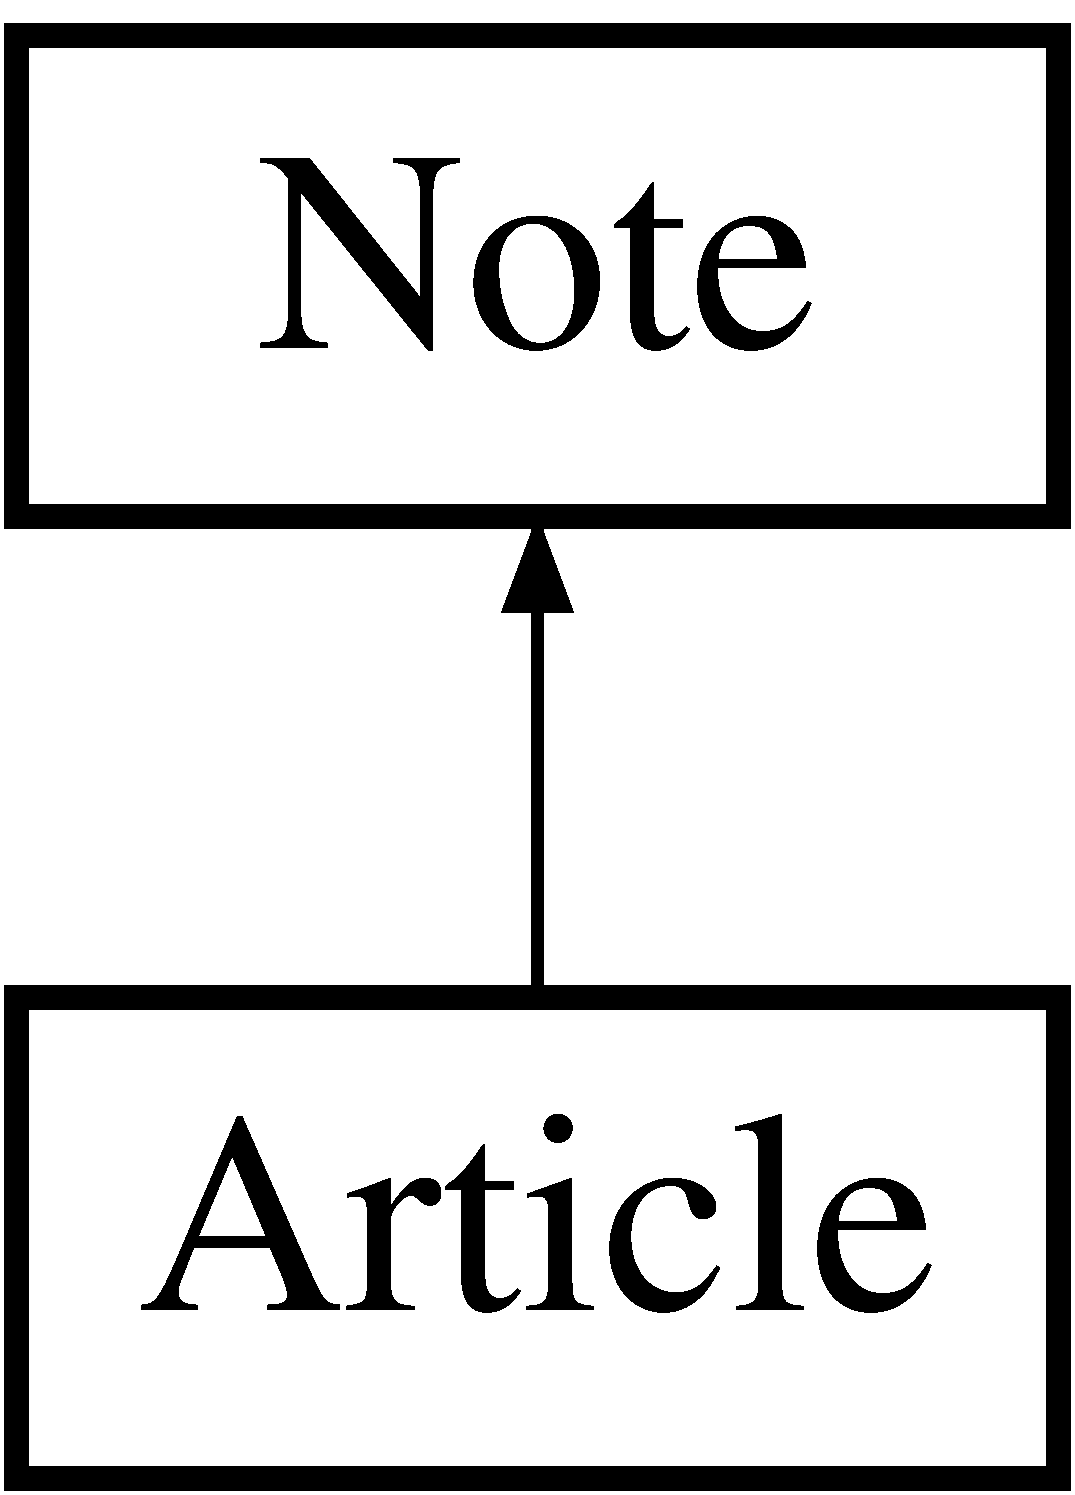
\includegraphics[height=2.000000cm]{class_article}
\end{center}
\end{figure}
\subsection*{Fonctions membres publiques}
\begin{DoxyCompactItemize}
\item 
Q\-String \hyperlink{class_article_a5aca02545dd453381abba632d7e05402}{get\-Texte} () const 
\begin{DoxyCompactList}\small\item\em get\-Texte \end{DoxyCompactList}\end{DoxyCompactItemize}
\subsection*{Fonctions membres protégées}
\begin{DoxyCompactItemize}
\item 
\hyperlink{class_article_ac7e17d78ceb14b64c0781a5caa83ef0a}{Article} (Q\-String id, Q\-String t, Q\-String text, Q\-Date date\-\_\-c=Q\-Date\-::current\-Date(), Q\-Date date\-\_\-m=Q\-Date\-::current\-Date(), unsigned int v=1, bool last=true, Note\-Etat e=active)
\begin{DoxyCompactList}\small\item\em Constructeur d'un article. \end{DoxyCompactList}\end{DoxyCompactItemize}
\subsection*{Attributs protégés}
\begin{DoxyCompactItemize}
\item 
\hypertarget{class_article_ab75a1cc11324d419d62e3114a462d31d}{Q\-String {\bfseries texte}}\label{class_article_ab75a1cc11324d419d62e3114a462d31d}

\end{DoxyCompactItemize}
\subsection*{Amis}
\begin{DoxyCompactItemize}
\item 
\hypertarget{class_article_a017a5144e8cfa6087305055ab968ef41}{class {\bfseries Notes\-Manager}}\label{class_article_a017a5144e8cfa6087305055ab968ef41}

\item 
\hypertarget{class_article_a7c44822b658a328771753fe0aaa8b7ae}{class {\bfseries Vue\-Principale}}\label{class_article_a7c44822b658a328771753fe0aaa8b7ae}

\end{DoxyCompactItemize}


\subsection{Description détaillée}
Représente un article. 

\subsection{Documentation des constructeurs et destructeur}
\hypertarget{class_article_ac7e17d78ceb14b64c0781a5caa83ef0a}{\index{Article@{Article}!Article@{Article}}
\index{Article@{Article}!Article@{Article}}
\subsubsection[{Article}]{\setlength{\rightskip}{0pt plus 5cm}Article\-::\-Article (
\begin{DoxyParamCaption}
\item[{Q\-String}]{id, }
\item[{Q\-String}]{t, }
\item[{Q\-String}]{text, }
\item[{Q\-Date}]{date\-\_\-c = {\ttfamily QDate\-:\-:currentDate()}, }
\item[{Q\-Date}]{date\-\_\-m = {\ttfamily QDate\-:\-:currentDate()}, }
\item[{unsigned int}]{v = {\ttfamily 1}, }
\item[{bool}]{last = {\ttfamily true}, }
\item[{Note\-Etat}]{e = {\ttfamily active}}
\end{DoxyParamCaption}
)\hspace{0.3cm}{\ttfamily [inline]}, {\ttfamily [protected]}}}\label{class_article_ac7e17d78ceb14b64c0781a5caa83ef0a}


Constructeur d'un article. 


\begin{DoxyParams}{Paramètres}
{\em id} & L'identificateur de la note \\
\hline
{\em t} & Le titre de la note \\
\hline
{\em date\-\_\-c} & La date de création \\
\hline
{\em date\-\_\-m} & La date de dernière modification \\
\hline
{\em last} & Indique si c'est la dernière version de la note ou pas \\
\hline
{\em v} & Version de la note \\
\hline
{\em e} & Etat de la note (active, archivée ou corbeille). \\
\hline
{\em text} & Le contenu de l'article. \\
\hline
\end{DoxyParams}


\subsection{Documentation des fonctions membres}
\hypertarget{class_article_a5aca02545dd453381abba632d7e05402}{\index{Article@{Article}!get\-Texte@{get\-Texte}}
\index{get\-Texte@{get\-Texte}!Article@{Article}}
\subsubsection[{get\-Texte}]{\setlength{\rightskip}{0pt plus 5cm}Q\-String Article\-::get\-Texte (
\begin{DoxyParamCaption}
{}
\end{DoxyParamCaption}
) const\hspace{0.3cm}{\ttfamily [inline]}}}\label{class_article_a5aca02545dd453381abba632d7e05402}


get\-Texte 

\begin{DoxyReturn}{Renvoie}
Retourne le contenu de l'article 
\end{DoxyReturn}


La documentation de cette classe a été générée à partir des fichiers suivants \-:\begin{DoxyCompactItemize}
\item 
/home/camille/\-Documents/\-U\-T\-C/\-H\-U04/\-L\-O21/\-Projet/\-Projet/\hyperlink{note_8h}{note.\-h}\item 
/home/camille/\-Documents/\-U\-T\-C/\-H\-U04/\-L\-O21/\-Projet/\-Projet/\hyperlink{note_8cpp}{note.\-cpp}\end{DoxyCompactItemize}

\hypertarget{class_article_editeur}{\section{Référence de la classe Article\-Editeur}
\label{class_article_editeur}\index{Article\-Editeur@{Article\-Editeur}}
}


Permet de visualiser et modifier les articles (interface).  




{\ttfamily \#include $<$noteediteur.\-h$>$}

Graphe d'héritage de Article\-Editeur\-:\begin{figure}[H]
\begin{center}
\leavevmode
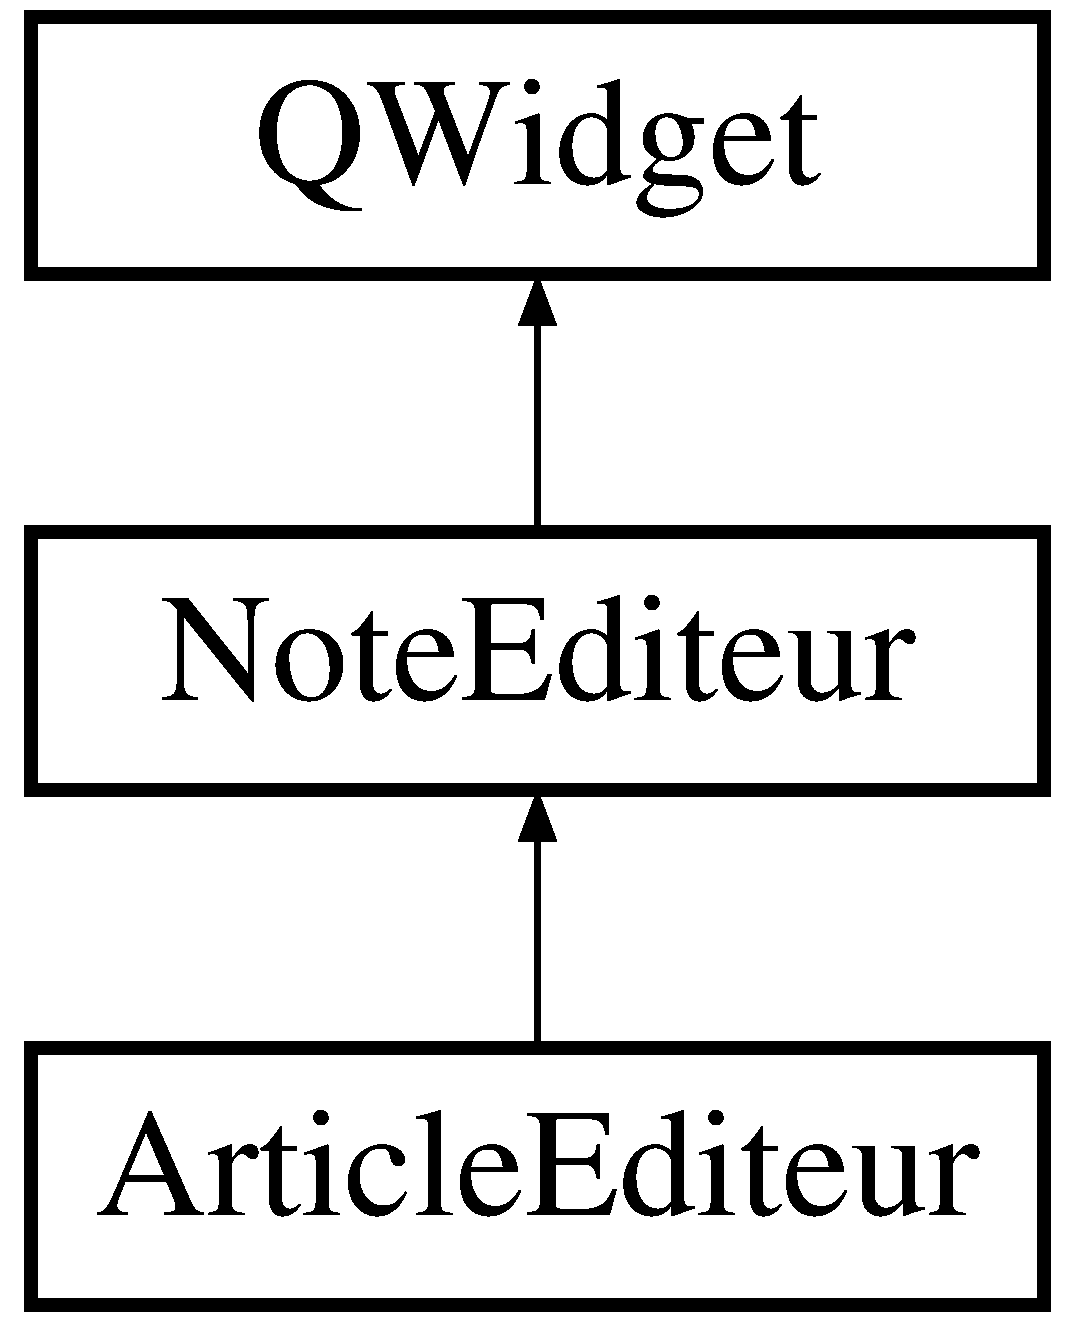
\includegraphics[height=3.000000cm]{class_article_editeur}
\end{center}
\end{figure}
\subsection*{Connecteurs publics}
\begin{DoxyCompactItemize}
\item 
\hypertarget{class_article_editeur_aa4898bacb77aeedde71e42e913fe2ef1}{void \hyperlink{class_article_editeur_aa4898bacb77aeedde71e42e913fe2ef1}{extensionsave} ()}\label{class_article_editeur_aa4898bacb77aeedde71e42e913fe2ef1}

\begin{DoxyCompactList}\small\item\em Définit la sauvegarde selon la sous-\/classe de note (appelée par \hyperlink{class_note_editeur_a605b1bca885c25460cb7d8863d1f3d03}{save()}) \end{DoxyCompactList}\item 
\hypertarget{class_article_editeur_ad7a90d03ed2b3b68821922d163572164}{void \hyperlink{class_article_editeur_ad7a90d03ed2b3b68821922d163572164}{extensionsetasactual} ()}\label{class_article_editeur_ad7a90d03ed2b3b68821922d163572164}

\begin{DoxyCompactList}\small\item\em Définit l'actualisation selon la sous-\/classe de la note (appelée par \hyperlink{class_note_editeur_a857f285628a0b7dcb6a69b18c977aa71}{set\-As\-Actual()}) \end{DoxyCompactList}\item 
\hypertarget{class_article_editeur_aeef410ab65c43484e0a39a71c65f7883}{void \hyperlink{class_article_editeur_aeef410ab65c43484e0a39a71c65f7883}{create} ()}\label{class_article_editeur_aeef410ab65c43484e0a39a71c65f7883}

\begin{DoxyCompactList}\small\item\em Création d'un nouvel objet article depuis l'article\-Editeur. \end{DoxyCompactList}\end{DoxyCompactItemize}
\subsection*{Fonctions membres publiques}
\begin{DoxyCompactItemize}
\item 
\hyperlink{class_article_editeur_abe5a564e7ba1af7d18a8787cd5936138}{Article\-Editeur} (\hyperlink{class_article}{Article} \&a, Q\-Widget $\ast$parent=0)
\begin{DoxyCompactList}\small\item\em Constructeur. \end{DoxyCompactList}\item 
\hyperlink{class_article_editeur_ae6fa307a670850f56cb20a96999f9a14}{Article\-Editeur} (Q\-Widget $\ast$parent=0)
\begin{DoxyCompactList}\small\item\em Surcharge de constructeur. \end{DoxyCompactList}\item 
\hypertarget{class_article_editeur_ade4f5d8bb85d0f1bfad9535f33174446}{void \hyperlink{class_article_editeur_ade4f5d8bb85d0f1bfad9535f33174446}{blockall} ()}\label{class_article_editeur_ade4f5d8bb85d0f1bfad9535f33174446}

\begin{DoxyCompactList}\small\item\em Permet d'interdire toute action à l'utilisateur (désactive tous les boutons) \end{DoxyCompactList}\end{DoxyCompactItemize}
\subsection*{Attributs protégés}
\begin{DoxyCompactItemize}
\item 
\hypertarget{class_article_editeur_a035b1dc25ffe1ac4bea73834d50f81b8}{Q\-Label $\ast$ {\bfseries text1}}\label{class_article_editeur_a035b1dc25ffe1ac4bea73834d50f81b8}

\item 
\hypertarget{class_article_editeur_a3af526051de08d1540ca694e672a5979}{Q\-Text\-Edit $\ast$ {\bfseries text}}\label{class_article_editeur_a3af526051de08d1540ca694e672a5979}

\end{DoxyCompactItemize}


\subsection{Description détaillée}
Permet de visualiser et modifier les articles (interface). 

Classe qui est par la suite utilisée pour réaliser l'ensemble de l'interface graphiue (\hyperlink{interface_8h}{interface.\-h}). 

\subsection{Documentation des constructeurs et destructeur}
\hypertarget{class_article_editeur_abe5a564e7ba1af7d18a8787cd5936138}{\index{Article\-Editeur@{Article\-Editeur}!Article\-Editeur@{Article\-Editeur}}
\index{Article\-Editeur@{Article\-Editeur}!ArticleEditeur@{Article\-Editeur}}
\subsubsection[{Article\-Editeur}]{\setlength{\rightskip}{0pt plus 5cm}Article\-Editeur\-::\-Article\-Editeur (
\begin{DoxyParamCaption}
\item[{{\bf Article} \&}]{a, }
\item[{Q\-Widget $\ast$}]{parent = {\ttfamily 0}}
\end{DoxyParamCaption}
)}}\label{class_article_editeur_abe5a564e7ba1af7d18a8787cd5936138}


Constructeur. 


\begin{DoxyParams}{Paramètres}
{\em a} & \hyperlink{class_article}{Article} à afficher \\
\hline
\end{DoxyParams}
\hypertarget{class_article_editeur_ae6fa307a670850f56cb20a96999f9a14}{\index{Article\-Editeur@{Article\-Editeur}!Article\-Editeur@{Article\-Editeur}}
\index{Article\-Editeur@{Article\-Editeur}!ArticleEditeur@{Article\-Editeur}}
\subsubsection[{Article\-Editeur}]{\setlength{\rightskip}{0pt plus 5cm}Article\-Editeur\-::\-Article\-Editeur (
\begin{DoxyParamCaption}
\item[{Q\-Widget $\ast$}]{parent = {\ttfamily 0}}
\end{DoxyParamCaption}
)}}\label{class_article_editeur_ae6fa307a670850f56cb20a96999f9a14}


Surcharge de constructeur. 

Si l'on n'a pas d'article à afficher (éditeur par défaut, vide). 
\begin{DoxyParams}{Paramètres}
{\em a} & \hyperlink{class_article}{Article} à afficher \\
\hline
\end{DoxyParams}


La documentation de cette classe a été générée à partir des fichiers suivants \-:\begin{DoxyCompactItemize}
\item 
/home/camille/\-Documents/\-U\-T\-C/\-H\-U04/\-L\-O21/\-Projet/\-Projet/\hyperlink{noteediteur_8h}{noteediteur.\-h}\item 
/home/camille/\-Documents/\-U\-T\-C/\-H\-U04/\-L\-O21/\-Projet/\-Projet/noteediteur.\-cpp\end{DoxyCompactItemize}

\hypertarget{class_fichier}{\section{Référence de la classe Fichier}
\label{class_fichier}\index{Fichier@{Fichier}}
}


Représente un fichier (image, audio ou vidéo).  




{\ttfamily \#include $<$note.\-h$>$}

Graphe d'héritage de Fichier\-:\begin{figure}[H]
\begin{center}
\leavevmode
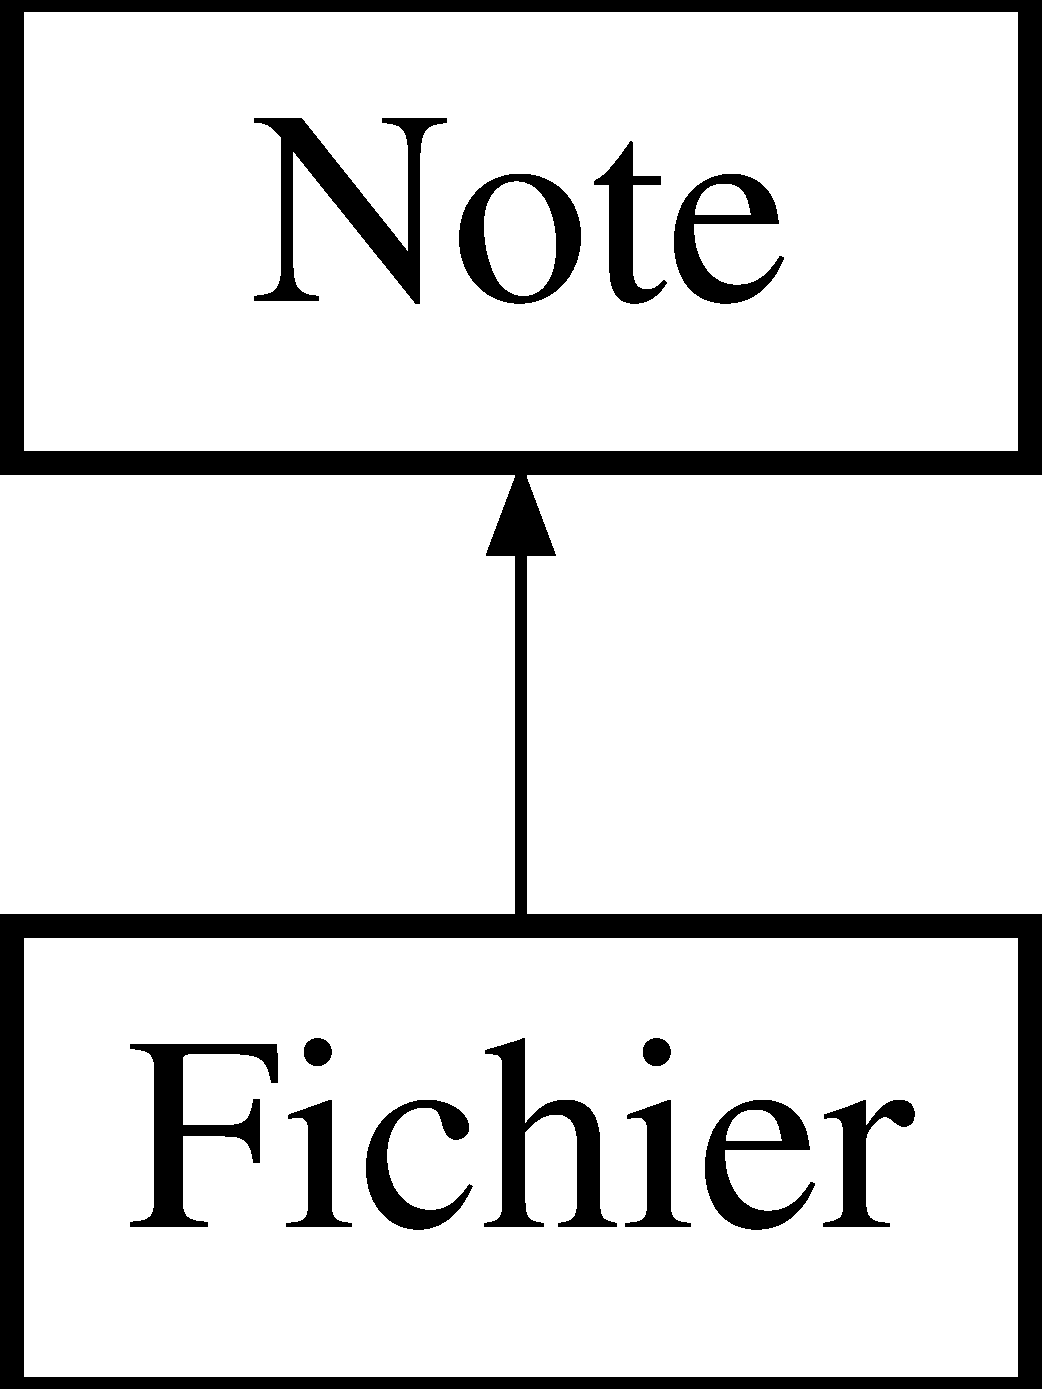
\includegraphics[height=2.000000cm]{class_fichier}
\end{center}
\end{figure}
\subsection*{Fonctions membres publiques}
\begin{DoxyCompactItemize}
\item 
Q\-String \hyperlink{class_fichier_ae8a21cbcf691006c9bf5d1a9cf3c039c}{get\-Description} () const 
\begin{DoxyCompactList}\small\item\em get\-Description \end{DoxyCompactList}\item 
Fichier\-Type \hyperlink{class_fichier_aea8a0b2ea4bf243166ee3b62214d3d3b}{get\-Type} () const 
\begin{DoxyCompactList}\small\item\em get\-Type \end{DoxyCompactList}\item 
Q\-String \hyperlink{class_fichier_ab1f7b30f9fc66ff24c97f65a2956609f}{get\-Filename} () const 
\begin{DoxyCompactList}\small\item\em get\-Filename \end{DoxyCompactList}\end{DoxyCompactItemize}
\subsection*{Fonctions membres protégées}
\begin{DoxyCompactItemize}
\item 
\hyperlink{class_fichier_a7c16ae9e09cd4a3087b084e3328fbb06}{Fichier} (Q\-String id, Q\-String t, Fichier\-Type ty, Q\-String descr, Q\-String name=\char`\"{}\char`\"{}, Q\-Date date\-\_\-c=Q\-Date\-::current\-Date(), Q\-Date date\-\_\-m=Q\-Date\-::current\-Date(), bool last=true, int v=1, Note\-Etat e=active)
\begin{DoxyCompactList}\small\item\em Constructeur d'une note. \end{DoxyCompactList}\end{DoxyCompactItemize}
\subsection*{Attributs protégés}
\begin{DoxyCompactItemize}
\item 
\hypertarget{class_fichier_af114aab83c1ffc271f2eeb91b8947b15}{Fichier\-Type {\bfseries type}}\label{class_fichier_af114aab83c1ffc271f2eeb91b8947b15}

\item 
\hypertarget{class_fichier_a6d157ead0d4cde6d7cf1f8723dc52d46}{Q\-String {\bfseries description}}\label{class_fichier_a6d157ead0d4cde6d7cf1f8723dc52d46}

\item 
\hypertarget{class_fichier_adf194796fa81d9d971a6b2ab793c8b29}{Q\-String {\bfseries filename}}\label{class_fichier_adf194796fa81d9d971a6b2ab793c8b29}

\end{DoxyCompactItemize}
\subsection*{Amis}
\begin{DoxyCompactItemize}
\item 
\hypertarget{class_fichier_a017a5144e8cfa6087305055ab968ef41}{class {\bfseries Notes\-Manager}}\label{class_fichier_a017a5144e8cfa6087305055ab968ef41}

\end{DoxyCompactItemize}


\subsection{Description détaillée}
Représente un fichier (image, audio ou vidéo). 

\subsection{Documentation des constructeurs et destructeur}
\hypertarget{class_fichier_a7c16ae9e09cd4a3087b084e3328fbb06}{\index{Fichier@{Fichier}!Fichier@{Fichier}}
\index{Fichier@{Fichier}!Fichier@{Fichier}}
\subsubsection[{Fichier}]{\setlength{\rightskip}{0pt plus 5cm}Fichier\-::\-Fichier (
\begin{DoxyParamCaption}
\item[{Q\-String}]{id, }
\item[{Q\-String}]{t, }
\item[{Fichier\-Type}]{ty, }
\item[{Q\-String}]{descr, }
\item[{Q\-String}]{name = {\ttfamily \char`\"{}\char`\"{}}, }
\item[{Q\-Date}]{date\-\_\-c = {\ttfamily QDate\-:\-:currentDate()}, }
\item[{Q\-Date}]{date\-\_\-m = {\ttfamily QDate\-:\-:currentDate()}, }
\item[{bool}]{last = {\ttfamily true}, }
\item[{int}]{v = {\ttfamily 1}, }
\item[{Note\-Etat}]{e = {\ttfamily active}}
\end{DoxyParamCaption}
)\hspace{0.3cm}{\ttfamily [inline]}, {\ttfamily [protected]}}}\label{class_fichier_a7c16ae9e09cd4a3087b084e3328fbb06}


Constructeur d'une note. 


\begin{DoxyParams}{Paramètres}
{\em id} & L'identificateur de la note \\
\hline
{\em t} & Le titre de la note \\
\hline
{\em date\-\_\-c} & La date de création \\
\hline
{\em date\-\_\-m} & La date de dernière modification \\
\hline
{\em last} & Indique si c'est la dernière version de la note ou pas \\
\hline
{\em v} & Version de la note \\
\hline
{\em e} & Etat de la note (active, archivée ou corbeille). \\
\hline
{\em ty} & Type de la note (image, audio, video) \\
\hline
{\em descr} & Description \\
\hline
{\em name} & Nom du fichier. \\
\hline
\end{DoxyParams}


\subsection{Documentation des fonctions membres}
\hypertarget{class_fichier_ae8a21cbcf691006c9bf5d1a9cf3c039c}{\index{Fichier@{Fichier}!get\-Description@{get\-Description}}
\index{get\-Description@{get\-Description}!Fichier@{Fichier}}
\subsubsection[{get\-Description}]{\setlength{\rightskip}{0pt plus 5cm}Q\-String Fichier\-::get\-Description (
\begin{DoxyParamCaption}
{}
\end{DoxyParamCaption}
) const\hspace{0.3cm}{\ttfamily [inline]}}}\label{class_fichier_ae8a21cbcf691006c9bf5d1a9cf3c039c}


get\-Description 

\begin{DoxyReturn}{Renvoie}
La description 
\end{DoxyReturn}
\hypertarget{class_fichier_ab1f7b30f9fc66ff24c97f65a2956609f}{\index{Fichier@{Fichier}!get\-Filename@{get\-Filename}}
\index{get\-Filename@{get\-Filename}!Fichier@{Fichier}}
\subsubsection[{get\-Filename}]{\setlength{\rightskip}{0pt plus 5cm}Q\-String Fichier\-::get\-Filename (
\begin{DoxyParamCaption}
{}
\end{DoxyParamCaption}
) const\hspace{0.3cm}{\ttfamily [inline]}}}\label{class_fichier_ab1f7b30f9fc66ff24c97f65a2956609f}


get\-Filename 

\begin{DoxyReturn}{Renvoie}
Le nom du fichier. 
\end{DoxyReturn}
\hypertarget{class_fichier_aea8a0b2ea4bf243166ee3b62214d3d3b}{\index{Fichier@{Fichier}!get\-Type@{get\-Type}}
\index{get\-Type@{get\-Type}!Fichier@{Fichier}}
\subsubsection[{get\-Type}]{\setlength{\rightskip}{0pt plus 5cm}Fichier\-Type Fichier\-::get\-Type (
\begin{DoxyParamCaption}
{}
\end{DoxyParamCaption}
) const\hspace{0.3cm}{\ttfamily [inline]}}}\label{class_fichier_aea8a0b2ea4bf243166ee3b62214d3d3b}


get\-Type 

\begin{DoxyReturn}{Renvoie}
Le type (image, audio, video) 
\end{DoxyReturn}


La documentation de cette classe a été générée à partir des fichiers suivants \-:\begin{DoxyCompactItemize}
\item 
/home/camille/\-Documents/\-U\-T\-C/\-H\-U04/\-L\-O21/\-Projet/\-Projet/\hyperlink{note_8h}{note.\-h}\item 
/home/camille/\-Documents/\-U\-T\-C/\-H\-U04/\-L\-O21/\-Projet/\-Projet/\hyperlink{note_8cpp}{note.\-cpp}\end{DoxyCompactItemize}

\hypertarget{class_fichier_editeur}{\section{Référence de la classe Fichier\-Editeur}
\label{class_fichier_editeur}\index{Fichier\-Editeur@{Fichier\-Editeur}}
}


Permet de visualiser et modifier les images, vidéos et fichiers audios (interface).  




{\ttfamily \#include $<$noteediteur.\-h$>$}

Graphe d'héritage de Fichier\-Editeur\-:\begin{figure}[H]
\begin{center}
\leavevmode
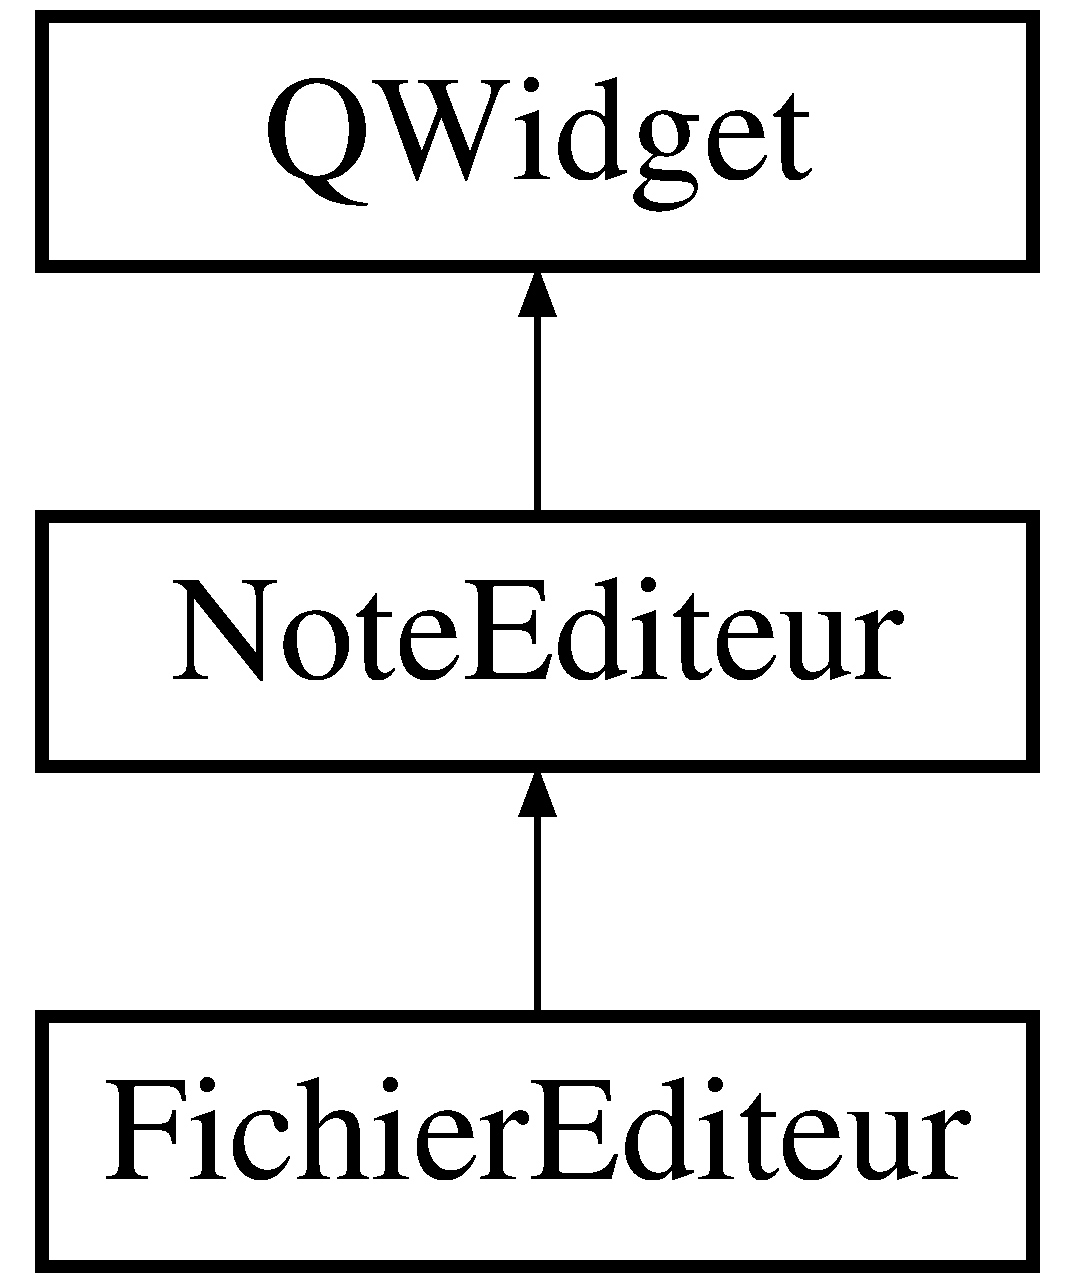
\includegraphics[height=3.000000cm]{class_fichier_editeur}
\end{center}
\end{figure}
\subsection*{Connecteurs publics}
\begin{DoxyCompactItemize}
\item 
\hypertarget{class_fichier_editeur_a1ab7b70f3f0cad780738c7307153a6da}{void \hyperlink{class_fichier_editeur_a1ab7b70f3f0cad780738c7307153a6da}{extensionsave} ()}\label{class_fichier_editeur_a1ab7b70f3f0cad780738c7307153a6da}

\begin{DoxyCompactList}\small\item\em Définit la sauvegarde selon la sous-\/classe de note (appelée par \hyperlink{class_note_editeur_a605b1bca885c25460cb7d8863d1f3d03}{save()}) \end{DoxyCompactList}\item 
\hypertarget{class_fichier_editeur_aff752c846d91e0b368b2fa6c90ad7bd0}{void \hyperlink{class_fichier_editeur_aff752c846d91e0b368b2fa6c90ad7bd0}{extensionsetasactual} ()}\label{class_fichier_editeur_aff752c846d91e0b368b2fa6c90ad7bd0}

\begin{DoxyCompactList}\small\item\em Définit l'actualisation selon la sous-\/classe de la note (appelée par \hyperlink{class_note_editeur_a857f285628a0b7dcb6a69b18c977aa71}{set\-As\-Actual()}) \end{DoxyCompactList}\item 
\hypertarget{class_fichier_editeur_adba804d5e299736d749696e0f7d554a9}{void \hyperlink{class_fichier_editeur_adba804d5e299736d749696e0f7d554a9}{create} ()}\label{class_fichier_editeur_adba804d5e299736d749696e0f7d554a9}

\begin{DoxyCompactList}\small\item\em Création d'un nouvel objet fichier depuis le fichier\-Editeur. \end{DoxyCompactList}\item 
void \hyperlink{class_fichier_editeur_a1cab6a95ce1ba94430b990cf5b5151ff}{select\-\_\-file} ()
\begin{DoxyCompactList}\small\item\em Permet d'ouvrir une fenêtre de dialogue d'ouverture de fihcier. \end{DoxyCompactList}\end{DoxyCompactItemize}
\subsection*{Fonctions membres publiques}
\begin{DoxyCompactItemize}
\item 
\hyperlink{class_fichier_editeur_a21dd5dd8fdb8564a3015956226339102}{Fichier\-Editeur} (\hyperlink{class_fichier}{Fichier} \&f, Q\-Widget $\ast$parent=0)
\begin{DoxyCompactList}\small\item\em Constructeur. \end{DoxyCompactList}\item 
\hypertarget{class_fichier_editeur_aee157b3bd8cea8a662a9c4a9c6a8d321}{\hyperlink{class_fichier_editeur_aee157b3bd8cea8a662a9c4a9c6a8d321}{Fichier\-Editeur} (Q\-Widget $\ast$parent=0)}\label{class_fichier_editeur_aee157b3bd8cea8a662a9c4a9c6a8d321}

\begin{DoxyCompactList}\small\item\em Surcharge de constructeur si on n'a pas de fichier à afficher. \end{DoxyCompactList}\item 
\hypertarget{class_fichier_editeur_a510e47495af4999ccbe2a40f05ff0db7}{void \hyperlink{class_fichier_editeur_a510e47495af4999ccbe2a40f05ff0db7}{blockall} ()}\label{class_fichier_editeur_a510e47495af4999ccbe2a40f05ff0db7}

\begin{DoxyCompactList}\small\item\em Permet d'interdire toute action à l'utilisateur (désactive tous les boutons) \end{DoxyCompactList}\end{DoxyCompactItemize}
\subsection*{Attributs protégés}
\begin{DoxyCompactItemize}
\item 
\hypertarget{class_fichier_editeur_a29d2d5135bb48badab92e03fdfffc9a5}{Q\-Radio\-Button $\ast$ {\bfseries type\-\_\-image}}\label{class_fichier_editeur_a29d2d5135bb48badab92e03fdfffc9a5}

\item 
\hypertarget{class_fichier_editeur_a68a59aa71966220c2c6c16622b972130}{Q\-Radio\-Button $\ast$ {\bfseries type\-\_\-audio}}\label{class_fichier_editeur_a68a59aa71966220c2c6c16622b972130}

\item 
\hypertarget{class_fichier_editeur_a79c110c29a393c010cc679035b5f8d3f}{Q\-Radio\-Button $\ast$ {\bfseries type\-\_\-video}}\label{class_fichier_editeur_a79c110c29a393c010cc679035b5f8d3f}

\item 
\hypertarget{class_fichier_editeur_a3520056824eb29126803983bfbdc129c}{Q\-Label $\ast$ {\bfseries description1}}\label{class_fichier_editeur_a3520056824eb29126803983bfbdc129c}

\item 
\hypertarget{class_fichier_editeur_a6185e187b00202c2dc295968051d0bf6}{Q\-Text\-Edit $\ast$ {\bfseries description}}\label{class_fichier_editeur_a6185e187b00202c2dc295968051d0bf6}

\item 
\hypertarget{class_fichier_editeur_a87fa51b2a2735aea2ecc10ead7147f05}{Q\-Push\-Button $\ast$ {\bfseries select}}\label{class_fichier_editeur_a87fa51b2a2735aea2ecc10ead7147f05}

\item 
\hypertarget{class_fichier_editeur_a07ef317838283ad412ed4d3e8490bc14}{Q\-Label $\ast$ {\bfseries filename1}}\label{class_fichier_editeur_a07ef317838283ad412ed4d3e8490bc14}

\item 
\hypertarget{class_fichier_editeur_adae6b25e1ff532a32f527feb0ffc1bf6}{Q\-String {\bfseries filename}}\label{class_fichier_editeur_adae6b25e1ff532a32f527feb0ffc1bf6}

\item 
\hypertarget{class_fichier_editeur_a0d5b61a262009db6d9fb4321adf0906a}{Q\-Label $\ast$ {\bfseries label\-\_\-visu}}\label{class_fichier_editeur_a0d5b61a262009db6d9fb4321adf0906a}

\item 
\hypertarget{class_fichier_editeur_a6a32481f4a945ed6ddaeb463b74f5fbe}{Q\-Pixmap $\ast$ {\bfseries visu\-\_\-image}}\label{class_fichier_editeur_a6a32481f4a945ed6ddaeb463b74f5fbe}

\end{DoxyCompactItemize}


\subsection{Description détaillée}
Permet de visualiser et modifier les images, vidéos et fichiers audios (interface). 

Classe qui est par la suite utilisée pour réaliser l'ensemble de l'interface graphiue (\hyperlink{interface_8h}{interface.\-h}). 

\subsection{Documentation des constructeurs et destructeur}
\hypertarget{class_fichier_editeur_a21dd5dd8fdb8564a3015956226339102}{\index{Fichier\-Editeur@{Fichier\-Editeur}!Fichier\-Editeur@{Fichier\-Editeur}}
\index{Fichier\-Editeur@{Fichier\-Editeur}!FichierEditeur@{Fichier\-Editeur}}
\subsubsection[{Fichier\-Editeur}]{\setlength{\rightskip}{0pt plus 5cm}Fichier\-Editeur\-::\-Fichier\-Editeur (
\begin{DoxyParamCaption}
\item[{{\bf Fichier} \&}]{f, }
\item[{Q\-Widget $\ast$}]{parent = {\ttfamily 0}}
\end{DoxyParamCaption}
)}}\label{class_fichier_editeur_a21dd5dd8fdb8564a3015956226339102}


Constructeur. 


\begin{DoxyParams}{Paramètres}
{\em f} & \hyperlink{class_fichier}{Fichier} à afficer \\
\hline
\end{DoxyParams}


\subsection{Documentation des fonctions membres}
\hypertarget{class_fichier_editeur_a1cab6a95ce1ba94430b990cf5b5151ff}{\index{Fichier\-Editeur@{Fichier\-Editeur}!select\-\_\-file@{select\-\_\-file}}
\index{select\-\_\-file@{select\-\_\-file}!FichierEditeur@{Fichier\-Editeur}}
\subsubsection[{select\-\_\-file}]{\setlength{\rightskip}{0pt plus 5cm}void Fichier\-Editeur\-::select\-\_\-file (
\begin{DoxyParamCaption}
{}
\end{DoxyParamCaption}
)\hspace{0.3cm}{\ttfamily [slot]}}}\label{class_fichier_editeur_a1cab6a95ce1ba94430b990cf5b5151ff}


Permet d'ouvrir une fenêtre de dialogue d'ouverture de fihcier. 

Gère les différents types de fichiers (fenêtre de dialogue différente selon le type). 

La documentation de cette classe a été générée à partir des fichiers suivants \-:\begin{DoxyCompactItemize}
\item 
/home/camille/\-Documents/\-U\-T\-C/\-H\-U04/\-L\-O21/\-Projet/\-Projet/\hyperlink{noteediteur_8h}{noteediteur.\-h}\item 
/home/camille/\-Documents/\-U\-T\-C/\-H\-U04/\-L\-O21/\-Projet/\-Projet/noteediteur.\-cpp\end{DoxyCompactItemize}

\hypertarget{class_interface_exception}{\section{Référence de la classe Interface\-Exception}
\label{class_interface_exception}\index{Interface\-Exception@{Interface\-Exception}}
}


Permet de gérer les exceptions liées à l'interface.  




{\ttfamily \#include $<$interface.\-h$>$}

\subsection*{Fonctions membres publiques}
\begin{DoxyCompactItemize}
\item 
\hypertarget{class_interface_exception_a94c63025ff679efa69cf8878c3a34dad}{{\bfseries Interface\-Exception} (const Q\-String \&message)}\label{class_interface_exception_a94c63025ff679efa69cf8878c3a34dad}

\item 
\hypertarget{class_interface_exception_a1c0925063de4c7377fd1502c0470eb49}{Q\-String {\bfseries get\-Info} () const }\label{class_interface_exception_a1c0925063de4c7377fd1502c0470eb49}

\end{DoxyCompactItemize}
\subsection*{Attributs privés}
\begin{DoxyCompactItemize}
\item 
\hypertarget{class_interface_exception_a352de63c3f5105468e0129cdcdee48ee}{Q\-String {\bfseries info}}\label{class_interface_exception_a352de63c3f5105468e0129cdcdee48ee}

\end{DoxyCompactItemize}


\subsection{Description détaillée}
Permet de gérer les exceptions liées à l'interface. 

La documentation de cette classe a été générée à partir du fichier suivant \-:\begin{DoxyCompactItemize}
\item 
/home/camille/\-Documents/\-U\-T\-C/\-H\-U04/\-L\-O21/\-Projet/\-Projet/\hyperlink{interface_8h}{interface.\-h}\end{DoxyCompactItemize}

\hypertarget{class_relation_1_1_iterator}{\section{Référence de la classe Relation\-:\-:Iterator}
\label{class_relation_1_1_iterator}\index{Relation\-::\-Iterator@{Relation\-::\-Iterator}}
}
\subsection*{Fonctions membres publiques}
\begin{DoxyCompactItemize}
\item 
\hypertarget{class_relation_1_1_iterator_aa4c79c6d32dcdac36eb811571241c687}{\hyperlink{class_note}{Note} \& {\bfseries current\-\_\-note\-X} () const }\label{class_relation_1_1_iterator_aa4c79c6d32dcdac36eb811571241c687}

\item 
\hypertarget{class_relation_1_1_iterator_a41c4f483cc1128a7804bbd90ebdaf45e}{\hyperlink{class_note}{Note} \& {\bfseries current\-\_\-note\-Y} () const }\label{class_relation_1_1_iterator_a41c4f483cc1128a7804bbd90ebdaf45e}

\item 
\hypertarget{class_relation_1_1_iterator_a8ff276d2d33755160725b5dbc4a95a72}{void {\bfseries next} ()}\label{class_relation_1_1_iterator_a8ff276d2d33755160725b5dbc4a95a72}

\item 
\hypertarget{class_relation_1_1_iterator_a4e2f828ed25ce251c6b6c08dbf618372}{bool {\bfseries is\-Done} () const }\label{class_relation_1_1_iterator_a4e2f828ed25ce251c6b6c08dbf618372}

\item 
\hypertarget{class_relation_1_1_iterator_ad32460ec4bc8f8b3a38c64f8c7b57b8b}{void {\bfseries debut} ()}\label{class_relation_1_1_iterator_ad32460ec4bc8f8b3a38c64f8c7b57b8b}

\end{DoxyCompactItemize}
\subsection*{Fonctions membres privées}
\begin{DoxyCompactItemize}
\item 
\hypertarget{class_relation_1_1_iterator_a74986195817fbcd10909c05e39e2c595}{{\bfseries Iterator} (\hyperlink{class_note}{Note} $\ast$$\ast$$\ast$tab, unsigned int n)}\label{class_relation_1_1_iterator_a74986195817fbcd10909c05e39e2c595}

\end{DoxyCompactItemize}
\subsection*{Attributs privés}
\begin{DoxyCompactItemize}
\item 
\hypertarget{class_relation_1_1_iterator_aea16ae10fec907f4c7016afb373d78ab}{\hyperlink{class_note}{Note} $\ast$$\ast$$\ast$ {\bfseries notes}}\label{class_relation_1_1_iterator_aea16ae10fec907f4c7016afb373d78ab}

\item 
\hypertarget{class_relation_1_1_iterator_ace78ab8d273d1afddb1890d34731b252}{unsigned int {\bfseries courant}}\label{class_relation_1_1_iterator_ace78ab8d273d1afddb1890d34731b252}

\item 
\hypertarget{class_relation_1_1_iterator_ae498bfc50d1a75d085187ef08cce9b66}{unsigned int {\bfseries taille}}\label{class_relation_1_1_iterator_ae498bfc50d1a75d085187ef08cce9b66}

\end{DoxyCompactItemize}
\subsection*{Amis}
\begin{DoxyCompactItemize}
\item 
\hypertarget{class_relation_1_1_iterator_a7ee004262f27f8c916688911a71e3aa1}{class {\bfseries Relation}}\label{class_relation_1_1_iterator_a7ee004262f27f8c916688911a71e3aa1}

\end{DoxyCompactItemize}


La documentation de cette classe a été générée à partir du fichier suivant \-:\begin{DoxyCompactItemize}
\item 
/home/camille/\-Documents/\-U\-T\-C/\-H\-U04/\-L\-O21/\-Projet/\-Projet/\hyperlink{relation_8h}{relation.\-h}\end{DoxyCompactItemize}

\hypertarget{class_relations_manager_1_1_iterator}{\section{Référence de la classe Relations\-Manager\-:\-:Iterator}
\label{class_relations_manager_1_1_iterator}\index{Relations\-Manager\-::\-Iterator@{Relations\-Manager\-::\-Iterator}}
}
\subsection*{Fonctions membres publiques}
\begin{DoxyCompactItemize}
\item 
\hypertarget{class_relations_manager_1_1_iterator_a93b25cf6f66311125ff6f0c38e16470f}{\hyperlink{class_relation}{Relation} \& {\bfseries current} () const }\label{class_relations_manager_1_1_iterator_a93b25cf6f66311125ff6f0c38e16470f}

\item 
\hypertarget{class_relations_manager_1_1_iterator_a4a70812b8235c40bcbdf90555da917a0}{void {\bfseries next} ()}\label{class_relations_manager_1_1_iterator_a4a70812b8235c40bcbdf90555da917a0}

\item 
\hypertarget{class_relations_manager_1_1_iterator_a3a8654bc558d4f5830ffbb194a519c4c}{bool {\bfseries is\-Done} () const }\label{class_relations_manager_1_1_iterator_a3a8654bc558d4f5830ffbb194a519c4c}

\item 
\hypertarget{class_relations_manager_1_1_iterator_a1d2e1532c4a7634531af829743fbf68c}{void {\bfseries debut} ()}\label{class_relations_manager_1_1_iterator_a1d2e1532c4a7634531af829743fbf68c}

\end{DoxyCompactItemize}
\subsection*{Fonctions membres privées}
\begin{DoxyCompactItemize}
\item 
\hypertarget{class_relations_manager_1_1_iterator_ac11a54b8303123f1a3c81a36cfb16480}{{\bfseries Iterator} (\hyperlink{class_relation}{Relation} $\ast$$\ast$t, unsigned int n)}\label{class_relations_manager_1_1_iterator_ac11a54b8303123f1a3c81a36cfb16480}

\end{DoxyCompactItemize}
\subsection*{Attributs privés}
\begin{DoxyCompactItemize}
\item 
\hypertarget{class_relations_manager_1_1_iterator_ad4ead2ce335be1905114ae56ff2ff5f3}{\hyperlink{class_relation}{Relation} $\ast$$\ast$ {\bfseries tab}}\label{class_relations_manager_1_1_iterator_ad4ead2ce335be1905114ae56ff2ff5f3}

\item 
\hypertarget{class_relations_manager_1_1_iterator_a0c72dcf73bc29785ce74863b4aaa1386}{unsigned int {\bfseries courant}}\label{class_relations_manager_1_1_iterator_a0c72dcf73bc29785ce74863b4aaa1386}

\item 
\hypertarget{class_relations_manager_1_1_iterator_aef6b85f9ca5e1abfb072b133d9386b1a}{unsigned int {\bfseries taille}}\label{class_relations_manager_1_1_iterator_aef6b85f9ca5e1abfb072b133d9386b1a}

\end{DoxyCompactItemize}
\subsection*{Amis}
\begin{DoxyCompactItemize}
\item 
\hypertarget{class_relations_manager_1_1_iterator_ac617894445bd4f12c905741b1b4f9f6a}{class {\bfseries Relations\-Manager}}\label{class_relations_manager_1_1_iterator_ac617894445bd4f12c905741b1b4f9f6a}

\end{DoxyCompactItemize}


La documentation de cette classe a été générée à partir du fichier suivant \-:\begin{DoxyCompactItemize}
\item 
/home/camille/\-Documents/\-U\-T\-C/\-H\-U04/\-L\-O21/\-Projet/\-Projet/\hyperlink{relation_8h}{relation.\-h}\end{DoxyCompactItemize}

\hypertarget{class_notes_manager_1_1_iterator}{\section{Référence de la classe Notes\-Manager\-:\-:Iterator}
\label{class_notes_manager_1_1_iterator}\index{Notes\-Manager\-::\-Iterator@{Notes\-Manager\-::\-Iterator}}
}
\subsection*{Fonctions membres publiques}
\begin{DoxyCompactItemize}
\item 
\hypertarget{class_notes_manager_1_1_iterator_a08d0d561704a142e828416b39bbf1ccd}{\hyperlink{class_note}{Note} \& {\bfseries current} () const }\label{class_notes_manager_1_1_iterator_a08d0d561704a142e828416b39bbf1ccd}

\item 
\hypertarget{class_notes_manager_1_1_iterator_a1a79699fe56e691c3f1c72eb46703fc6}{void {\bfseries next} ()}\label{class_notes_manager_1_1_iterator_a1a79699fe56e691c3f1c72eb46703fc6}

\item 
\hypertarget{class_notes_manager_1_1_iterator_aca3037c7eac946bd34a98decb8f41051}{bool {\bfseries is\-Done} () const }\label{class_notes_manager_1_1_iterator_aca3037c7eac946bd34a98decb8f41051}

\item 
\hypertarget{class_notes_manager_1_1_iterator_a154ce8a4147ee99e2dcf93972a448fae}{void {\bfseries debut} ()}\label{class_notes_manager_1_1_iterator_a154ce8a4147ee99e2dcf93972a448fae}

\end{DoxyCompactItemize}
\subsection*{Fonctions membres privées}
\begin{DoxyCompactItemize}
\item 
\hypertarget{class_notes_manager_1_1_iterator_afb5a2182e04da56b1a0ddf3678b1c7c3}{{\bfseries Iterator} (\hyperlink{class_note}{Note} $\ast$$\ast$t, unsigned int n)}\label{class_notes_manager_1_1_iterator_afb5a2182e04da56b1a0ddf3678b1c7c3}

\end{DoxyCompactItemize}
\subsection*{Attributs privés}
\begin{DoxyCompactItemize}
\item 
\hypertarget{class_notes_manager_1_1_iterator_a5c9c9fbed536d945945dd0610730d7dd}{\hyperlink{class_note}{Note} $\ast$$\ast$ {\bfseries tab}}\label{class_notes_manager_1_1_iterator_a5c9c9fbed536d945945dd0610730d7dd}

\item 
\hypertarget{class_notes_manager_1_1_iterator_a850f87a5bd51749f482fef725f956af3}{unsigned int {\bfseries courant}}\label{class_notes_manager_1_1_iterator_a850f87a5bd51749f482fef725f956af3}

\item 
\hypertarget{class_notes_manager_1_1_iterator_a4384545d0df17a4003b9c5212aa4c64f}{unsigned int {\bfseries taille}}\label{class_notes_manager_1_1_iterator_a4384545d0df17a4003b9c5212aa4c64f}

\end{DoxyCompactItemize}
\subsection*{Amis}
\begin{DoxyCompactItemize}
\item 
\hypertarget{class_notes_manager_1_1_iterator_a017a5144e8cfa6087305055ab968ef41}{class {\bfseries Notes\-Manager}}\label{class_notes_manager_1_1_iterator_a017a5144e8cfa6087305055ab968ef41}

\end{DoxyCompactItemize}


La documentation de cette classe a été générée à partir du fichier suivant \-:\begin{DoxyCompactItemize}
\item 
/home/camille/\-Documents/\-U\-T\-C/\-H\-U04/\-L\-O21/\-Projet/\-Projet/\hyperlink{note_8h}{note.\-h}\end{DoxyCompactItemize}

\hypertarget{class_note}{\section{Référence de la classe Note}
\label{class_note}\index{Note@{Note}}
}


Classe abstraite représentant une note.  




{\ttfamily \#include $<$note.\-h$>$}

Graphe d'héritage de Note\-:\begin{figure}[H]
\begin{center}
\leavevmode
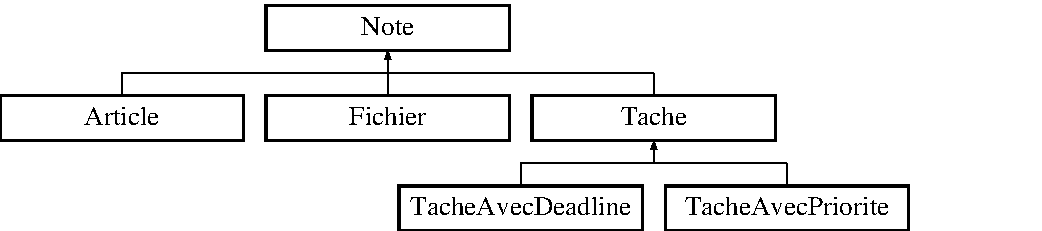
\includegraphics[height=3.000000cm]{class_note}
\end{center}
\end{figure}
\subsection*{Fonctions membres publiques}
\begin{DoxyCompactItemize}
\item 
Q\-String \hyperlink{class_note_a880a9b4330b29c7264e87a346d712ebc}{get\-Id} () const 
\begin{DoxyCompactList}\small\item\em get\-Id \end{DoxyCompactList}\item 
Q\-String \hyperlink{class_note_ad4e78b2146a88e8b5a253b9eeb496936}{get\-Titre} () const 
\begin{DoxyCompactList}\small\item\em get\-Titre \end{DoxyCompactList}\item 
Q\-Date \hyperlink{class_note_a23a61ddfcb6a5726cf43a40fb88d16aa}{get\-Creation} () const 
\begin{DoxyCompactList}\small\item\em get\-Creation \end{DoxyCompactList}\item 
Q\-Date \hyperlink{class_note_a3ff7b051ab009bf412b1c9ff99a62b27}{get\-Modification} () const 
\begin{DoxyCompactList}\small\item\em get\-Modification \end{DoxyCompactList}\item 
Note\-Etat \hyperlink{class_note_a55cd34f072d21f3b2f69133b2b6c5bf2}{get\-Etat} () const 
\begin{DoxyCompactList}\small\item\em get\-Etat \end{DoxyCompactList}\item 
bool \hyperlink{class_note_a55db384b5684c5d8dc6795424eda1d1a}{Is\-Last} () const 
\begin{DoxyCompactList}\small\item\em Is\-Last. \end{DoxyCompactList}\item 
unsigned int \hyperlink{class_note_a5a9830e6d44f86962ea54ee94480aa17}{get\-Version} () const 
\begin{DoxyCompactList}\small\item\em get\-Version \end{DoxyCompactList}\item 
void \hyperlink{class_note_acba9b05c587ff6a660a9b5c46614acf3}{set\-Last} (const bool b)
\begin{DoxyCompactList}\small\item\em permet de définir une version comme dernière ou pas. \end{DoxyCompactList}\item 
void \hyperlink{class_note_af4f439239e2f2dcdc9fb0abdac2bd67a}{set\-Etat} (Note\-Etat e)
\begin{DoxyCompactList}\small\item\em Permet de modifier l'état de la note. \end{DoxyCompactList}\end{DoxyCompactItemize}
\subsection*{Fonctions membres protégées}
\begin{DoxyCompactItemize}
\item 
\hyperlink{class_note_a1a696a0d5858ed217abc94a4c5640b7d}{Note} (Q\-String id, Q\-String t, Q\-Date date\-\_\-c=Q\-Date\-::current\-Date(), Q\-Date date\-\_\-m=Q\-Date\-::current\-Date(), bool last=true, unsigned int v=1, Note\-Etat e=active)
\begin{DoxyCompactList}\small\item\em Constructeur d'une note. \end{DoxyCompactList}\end{DoxyCompactItemize}
\subsection*{Attributs protégés}
\begin{DoxyCompactItemize}
\item 
\hypertarget{class_note_aacc7ebfda42d05b0dc5805ce9a9bcf73}{Q\-String {\bfseries identificateur}}\label{class_note_aacc7ebfda42d05b0dc5805ce9a9bcf73}

\item 
\hypertarget{class_note_a4f3aceb1ee03caa1f37a08880fe44f47}{Q\-String {\bfseries titre}}\label{class_note_a4f3aceb1ee03caa1f37a08880fe44f47}

\item 
\hypertarget{class_note_aa66b1aada95c18e3072dfcadb5137b20}{Q\-Date {\bfseries date\-\_\-creation}}\label{class_note_aa66b1aada95c18e3072dfcadb5137b20}

\item 
\hypertarget{class_note_a32dc337cdff9731eda7135426f87caf2}{Q\-Date {\bfseries date\-\_\-\-Lastmodification}}\label{class_note_a32dc337cdff9731eda7135426f87caf2}

\item 
\hypertarget{class_note_a081a30b2091a39a2c1a9da70a48df736}{bool {\bfseries is\-Last\-Version}}\label{class_note_a081a30b2091a39a2c1a9da70a48df736}

\item 
\hypertarget{class_note_a4d40f017d6f24cad4ae1f7c8046234df}{unsigned int {\bfseries version}}\label{class_note_a4d40f017d6f24cad4ae1f7c8046234df}

\item 
\hypertarget{class_note_ae81f84fc605e97173019e668744be3eb}{Note\-Etat {\bfseries etat}}\label{class_note_ae81f84fc605e97173019e668744be3eb}

\end{DoxyCompactItemize}
\subsection*{Amis}
\begin{DoxyCompactItemize}
\item 
\hypertarget{class_note_a017a5144e8cfa6087305055ab968ef41}{class {\bfseries Notes\-Manager}}\label{class_note_a017a5144e8cfa6087305055ab968ef41}

\end{DoxyCompactItemize}


\subsection{Description détaillée}
Classe abstraite représentant une note. 

\subsection{Documentation des constructeurs et destructeur}
\hypertarget{class_note_a1a696a0d5858ed217abc94a4c5640b7d}{\index{Note@{Note}!Note@{Note}}
\index{Note@{Note}!Note@{Note}}
\subsubsection[{Note}]{\setlength{\rightskip}{0pt plus 5cm}Note\-::\-Note (
\begin{DoxyParamCaption}
\item[{Q\-String}]{id, }
\item[{Q\-String}]{t, }
\item[{Q\-Date}]{date\-\_\-c = {\ttfamily QDate\-:\-:currentDate()}, }
\item[{Q\-Date}]{date\-\_\-m = {\ttfamily QDate\-:\-:currentDate()}, }
\item[{bool}]{last = {\ttfamily true}, }
\item[{unsigned int}]{v = {\ttfamily 1}, }
\item[{Note\-Etat}]{e = {\ttfamily active}}
\end{DoxyParamCaption}
)\hspace{0.3cm}{\ttfamily [inline]}, {\ttfamily [protected]}}}\label{class_note_a1a696a0d5858ed217abc94a4c5640b7d}


Constructeur d'une note. 


\begin{DoxyParams}{Paramètres}
{\em id} & L'identificateur de la note \\
\hline
{\em t} & Le titre de la note \\
\hline
{\em date\-\_\-c} & La date de création \\
\hline
{\em date\-\_\-m} & La date de dernière modification \\
\hline
{\em last} & Indique si c'est la dernière version de la note ou pas \\
\hline
{\em v} & Version de la note \\
\hline
{\em e} & Etat de la note (active, archivée ou corbeille). \\
\hline
\end{DoxyParams}


\subsection{Documentation des fonctions membres}
\hypertarget{class_note_a23a61ddfcb6a5726cf43a40fb88d16aa}{\index{Note@{Note}!get\-Creation@{get\-Creation}}
\index{get\-Creation@{get\-Creation}!Note@{Note}}
\subsubsection[{get\-Creation}]{\setlength{\rightskip}{0pt plus 5cm}Q\-Date Note\-::get\-Creation (
\begin{DoxyParamCaption}
{}
\end{DoxyParamCaption}
) const\hspace{0.3cm}{\ttfamily [inline]}}}\label{class_note_a23a61ddfcb6a5726cf43a40fb88d16aa}


get\-Creation 

\begin{DoxyReturn}{Renvoie}
Retourne la date de création de la note 
\end{DoxyReturn}
\hypertarget{class_note_a55cd34f072d21f3b2f69133b2b6c5bf2}{\index{Note@{Note}!get\-Etat@{get\-Etat}}
\index{get\-Etat@{get\-Etat}!Note@{Note}}
\subsubsection[{get\-Etat}]{\setlength{\rightskip}{0pt plus 5cm}Note\-Etat Note\-::get\-Etat (
\begin{DoxyParamCaption}
{}
\end{DoxyParamCaption}
) const\hspace{0.3cm}{\ttfamily [inline]}}}\label{class_note_a55cd34f072d21f3b2f69133b2b6c5bf2}


get\-Etat 

\begin{DoxyReturn}{Renvoie}
Retourne l'état de la note (active, archivée ou corbeille) 
\end{DoxyReturn}
\hypertarget{class_note_a880a9b4330b29c7264e87a346d712ebc}{\index{Note@{Note}!get\-Id@{get\-Id}}
\index{get\-Id@{get\-Id}!Note@{Note}}
\subsubsection[{get\-Id}]{\setlength{\rightskip}{0pt plus 5cm}Q\-String Note\-::get\-Id (
\begin{DoxyParamCaption}
{}
\end{DoxyParamCaption}
) const\hspace{0.3cm}{\ttfamily [inline]}}}\label{class_note_a880a9b4330b29c7264e87a346d712ebc}


get\-Id 

\begin{DoxyReturn}{Renvoie}
Retourne l'id de la note 
\end{DoxyReturn}
\hypertarget{class_note_a3ff7b051ab009bf412b1c9ff99a62b27}{\index{Note@{Note}!get\-Modification@{get\-Modification}}
\index{get\-Modification@{get\-Modification}!Note@{Note}}
\subsubsection[{get\-Modification}]{\setlength{\rightskip}{0pt plus 5cm}Q\-Date Note\-::get\-Modification (
\begin{DoxyParamCaption}
{}
\end{DoxyParamCaption}
) const\hspace{0.3cm}{\ttfamily [inline]}}}\label{class_note_a3ff7b051ab009bf412b1c9ff99a62b27}


get\-Modification 

\begin{DoxyReturn}{Renvoie}
Retourne la date de dernière modification de la note. 
\end{DoxyReturn}
\hypertarget{class_note_ad4e78b2146a88e8b5a253b9eeb496936}{\index{Note@{Note}!get\-Titre@{get\-Titre}}
\index{get\-Titre@{get\-Titre}!Note@{Note}}
\subsubsection[{get\-Titre}]{\setlength{\rightskip}{0pt plus 5cm}Q\-String Note\-::get\-Titre (
\begin{DoxyParamCaption}
{}
\end{DoxyParamCaption}
) const\hspace{0.3cm}{\ttfamily [inline]}}}\label{class_note_ad4e78b2146a88e8b5a253b9eeb496936}


get\-Titre 

\begin{DoxyReturn}{Renvoie}
Retourne le titre de la note 
\end{DoxyReturn}
\hypertarget{class_note_a5a9830e6d44f86962ea54ee94480aa17}{\index{Note@{Note}!get\-Version@{get\-Version}}
\index{get\-Version@{get\-Version}!Note@{Note}}
\subsubsection[{get\-Version}]{\setlength{\rightskip}{0pt plus 5cm}unsigned int Note\-::get\-Version (
\begin{DoxyParamCaption}
{}
\end{DoxyParamCaption}
) const\hspace{0.3cm}{\ttfamily [inline]}}}\label{class_note_a5a9830e6d44f86962ea54ee94480aa17}


get\-Version 

\begin{DoxyReturn}{Renvoie}
Retourne le numéro de la version 
\end{DoxyReturn}
\hypertarget{class_note_a55db384b5684c5d8dc6795424eda1d1a}{\index{Note@{Note}!Is\-Last@{Is\-Last}}
\index{Is\-Last@{Is\-Last}!Note@{Note}}
\subsubsection[{Is\-Last}]{\setlength{\rightskip}{0pt plus 5cm}bool Note\-::\-Is\-Last (
\begin{DoxyParamCaption}
{}
\end{DoxyParamCaption}
) const\hspace{0.3cm}{\ttfamily [inline]}}}\label{class_note_a55db384b5684c5d8dc6795424eda1d1a}


Is\-Last. 

\begin{DoxyReturn}{Renvoie}
True si c'est la dernière version, false sinon. 
\end{DoxyReturn}
\hypertarget{class_note_af4f439239e2f2dcdc9fb0abdac2bd67a}{\index{Note@{Note}!set\-Etat@{set\-Etat}}
\index{set\-Etat@{set\-Etat}!Note@{Note}}
\subsubsection[{set\-Etat}]{\setlength{\rightskip}{0pt plus 5cm}void Note\-::set\-Etat (
\begin{DoxyParamCaption}
\item[{Note\-Etat}]{e}
\end{DoxyParamCaption}
)\hspace{0.3cm}{\ttfamily [inline]}}}\label{class_note_af4f439239e2f2dcdc9fb0abdac2bd67a}


Permet de modifier l'état de la note. 


\begin{DoxyParams}{Paramètres}
{\em e} & Nouvel état de la note (active, archivée ou corbeille). \\
\hline
\end{DoxyParams}
\hypertarget{class_note_acba9b05c587ff6a660a9b5c46614acf3}{\index{Note@{Note}!set\-Last@{set\-Last}}
\index{set\-Last@{set\-Last}!Note@{Note}}
\subsubsection[{set\-Last}]{\setlength{\rightskip}{0pt plus 5cm}void Note\-::set\-Last (
\begin{DoxyParamCaption}
\item[{const bool}]{b}
\end{DoxyParamCaption}
)\hspace{0.3cm}{\ttfamily [inline]}}}\label{class_note_acba9b05c587ff6a660a9b5c46614acf3}


permet de définir une version comme dernière ou pas. 


\begin{DoxyParams}{Paramètres}
{\em b} & Vrai (si on veut définir la version comme dernière version) ou faux sinon. \\
\hline
\end{DoxyParams}


La documentation de cette classe a été générée à partir des fichiers suivants \-:\begin{DoxyCompactItemize}
\item 
/home/camille/\-Documents/\-U\-T\-C/\-H\-U04/\-L\-O21/\-Projet/\-Projet/\hyperlink{note_8h}{note.\-h}\item 
/home/camille/\-Documents/\-U\-T\-C/\-H\-U04/\-L\-O21/\-Projet/\-Projet/\hyperlink{note_8cpp}{note.\-cpp}\end{DoxyCompactItemize}

\hypertarget{class_note_editeur}{\section{Référence de la classe Note\-Editeur}
\label{class_note_editeur}\index{Note\-Editeur@{Note\-Editeur}}
}


Classe abstraite, permet de visualiser et modifier les notes (interface).  




{\ttfamily \#include $<$noteediteur.\-h$>$}

Graphe d'héritage de Note\-Editeur\-:\begin{figure}[H]
\begin{center}
\leavevmode
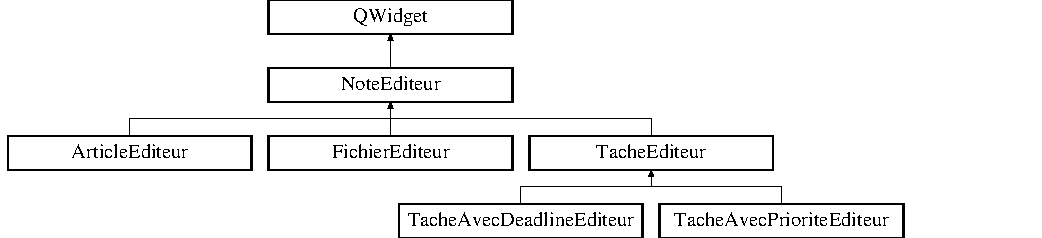
\includegraphics[height=3.200000cm]{class_note_editeur}
\end{center}
\end{figure}
\subsection*{Connecteurs publics}
\begin{DoxyCompactItemize}
\item 
\hypertarget{class_note_editeur_a605b1bca885c25460cb7d8863d1f3d03}{void \hyperlink{class_note_editeur_a605b1bca885c25460cb7d8863d1f3d03}{save} ()}\label{class_note_editeur_a605b1bca885c25460cb7d8863d1f3d03}

\begin{DoxyCompactList}\small\item\em Enregistre la note \& ses modifications. \end{DoxyCompactList}\item 
\hypertarget{class_note_editeur_a2918e7a3ddc7dfac7e2ce13589d00288}{void \hyperlink{class_note_editeur_a2918e7a3ddc7dfac7e2ce13589d00288}{delete\-\_\-note} ()}\label{class_note_editeur_a2918e7a3ddc7dfac7e2ce13589d00288}

\begin{DoxyCompactList}\small\item\em Supprime la note. \end{DoxyCompactList}\item 
\hypertarget{class_note_editeur_a857f285628a0b7dcb6a69b18c977aa71}{void \hyperlink{class_note_editeur_a857f285628a0b7dcb6a69b18c977aa71}{set\-As\-Actual} ()}\label{class_note_editeur_a857f285628a0b7dcb6a69b18c977aa71}

\begin{DoxyCompactList}\small\item\em Actualise la note. \end{DoxyCompactList}\item 
\hypertarget{class_note_editeur_a090e4299bb4ef113bb93d23d50d83bab}{void \hyperlink{class_note_editeur_a090e4299bb4ef113bb93d23d50d83bab}{restore} ()}\label{class_note_editeur_a090e4299bb4ef113bb93d23d50d83bab}

\begin{DoxyCompactList}\small\item\em Restaure une note. \end{DoxyCompactList}\end{DoxyCompactItemize}
\subsection*{Fonctions membres publiques}
\begin{DoxyCompactItemize}
\item 
\hyperlink{class_note_editeur_a83821d2de318dfa13a0cbbb321765101}{Note\-Editeur} (\hyperlink{class_note}{Note} \&n, Q\-Widget $\ast$parent=0)
\begin{DoxyCompactList}\small\item\em Constructeur. \end{DoxyCompactList}\item 
\hypertarget{class_note_editeur_a10b76711bf2e20d67fb7508a9dead555}{\hyperlink{class_note_editeur_a10b76711bf2e20d67fb7508a9dead555}{Note\-Editeur} (Q\-Widget $\ast$parent=0)}\label{class_note_editeur_a10b76711bf2e20d67fb7508a9dead555}

\begin{DoxyCompactList}\small\item\em Surcharge du constructeur si on souhaite l'afficher \char`\"{}vide\char`\"{} (sans note) \end{DoxyCompactList}\item 
\hypertarget{class_note_editeur_a1a47bd58dd1331be327a6693941970de}{Q\-V\-Box\-Layout $\ast$ \hyperlink{class_note_editeur_a1a47bd58dd1331be327a6693941970de}{get\-Layout} ()}\label{class_note_editeur_a1a47bd58dd1331be327a6693941970de}

\begin{DoxyCompactList}\small\item\em méthode pour récupérer le layout et le modifier en fonction de la sous-\/classe \end{DoxyCompactList}\item 
\hypertarget{class_note_editeur_a3244691035875af789abf64034e0c02a}{Q\-Push\-Button $\ast$ \hyperlink{class_note_editeur_a3244691035875af789abf64034e0c02a}{get\-Button\-\_\-save} ()}\label{class_note_editeur_a3244691035875af789abf64034e0c02a}

\begin{DoxyCompactList}\small\item\em Récupère le bouton save pour le modifier en fonction de la sous-\/classe. \end{DoxyCompactList}\item 
\hypertarget{class_note_editeur_ae5048eb415f3984cbb0c030a7f56d0fc}{Q\-Push\-Button $\ast$ \hyperlink{class_note_editeur_ae5048eb415f3984cbb0c030a7f56d0fc}{get\-Button\-\_\-delete} ()}\label{class_note_editeur_ae5048eb415f3984cbb0c030a7f56d0fc}

\begin{DoxyCompactList}\small\item\em Récupère le bouton delete pour le modifier en fonction de la sous-\/classe. \end{DoxyCompactList}\item 
\hypertarget{class_note_editeur_aed0e7526363691449376eab2beca1a00}{Q\-Push\-Button $\ast$ \hyperlink{class_note_editeur_aed0e7526363691449376eab2beca1a00}{get\-Button\-\_\-actualize} ()}\label{class_note_editeur_aed0e7526363691449376eab2beca1a00}

\begin{DoxyCompactList}\small\item\em Récupère le bouton actualiser pour le modifier en fonction de la sous-\/classe. \end{DoxyCompactList}\item 
\hypertarget{class_note_editeur_af781dd4dc8266aba4c1f462bd07f04b9}{Q\-Push\-Button $\ast$ \hyperlink{class_note_editeur_af781dd4dc8266aba4c1f462bd07f04b9}{get\-Button\-\_\-restore} ()}\label{class_note_editeur_af781dd4dc8266aba4c1f462bd07f04b9}

\begin{DoxyCompactList}\small\item\em Récupère le bouton restaurer pour le modifier en fonction de la sous-\/classe. \end{DoxyCompactList}\item 
\hypertarget{class_note_editeur_a33711732b03990dfa5333f1522625cdf}{Q\-Line\-Edit $\ast$ \hyperlink{class_note_editeur_a33711732b03990dfa5333f1522625cdf}{get\-Title} ()}\label{class_note_editeur_a33711732b03990dfa5333f1522625cdf}

\begin{DoxyCompactList}\small\item\em Récupère le titre pour le modifier en fonction de la sous-\/classe. \end{DoxyCompactList}\item 
\hypertarget{class_note_editeur_af10fb0bcfdf1ea508dd8e10a1ae9067b}{Q\-Line\-Edit $\ast$ \hyperlink{class_note_editeur_af10fb0bcfdf1ea508dd8e10a1ae9067b}{get\-Id} ()}\label{class_note_editeur_af10fb0bcfdf1ea508dd8e10a1ae9067b}

\begin{DoxyCompactList}\small\item\em Récupère l'id pour le modifier en fonction de la sous-\/classe. \end{DoxyCompactList}\item 
\hypertarget{class_note_editeur_a76120d7a97c881fc46e6874c3431ba32}{Q\-Label $\ast$ \hyperlink{class_note_editeur_a76120d7a97c881fc46e6874c3431ba32}{get\-Date\-\_\-m} ()}\label{class_note_editeur_a76120d7a97c881fc46e6874c3431ba32}

\begin{DoxyCompactList}\small\item\em Récupère la date de dernière modification. \end{DoxyCompactList}\item 
\hypertarget{class_note_editeur_ab8faf02aaffcb1290c9129b865e84180}{Q\-Label $\ast$ \hyperlink{class_note_editeur_ab8faf02aaffcb1290c9129b865e84180}{get\-Version} ()}\label{class_note_editeur_ab8faf02aaffcb1290c9129b865e84180}

\begin{DoxyCompactList}\small\item\em Récupère le numéro de version. \end{DoxyCompactList}\item 
\hypertarget{class_note_editeur_a1e1cee521fbbfb134f5b07b80996108d}{Q\-Label $\ast$ \hyperlink{class_note_editeur_a1e1cee521fbbfb134f5b07b80996108d}{get\-Last} ()}\label{class_note_editeur_a1e1cee521fbbfb134f5b07b80996108d}

\begin{DoxyCompactList}\small\item\em Vérifie si il s'agit de la dernière version de la note. \end{DoxyCompactList}\item 
\hypertarget{class_note_editeur_a35df5a555f5852f50ad8ca19f2e81bd1}{virtual void \hyperlink{class_note_editeur_a35df5a555f5852f50ad8ca19f2e81bd1}{extensionsave} ()=0}\label{class_note_editeur_a35df5a555f5852f50ad8ca19f2e81bd1}

\begin{DoxyCompactList}\small\item\em Définit la sauvegarde selon la sous-\/classe de note (appelée par \hyperlink{class_note_editeur_a605b1bca885c25460cb7d8863d1f3d03}{save()}) \end{DoxyCompactList}\item 
\hypertarget{class_note_editeur_a30bc10104ce0faac9d1261fcddd22589}{virtual void \hyperlink{class_note_editeur_a30bc10104ce0faac9d1261fcddd22589}{extensionsetasactual} ()=0}\label{class_note_editeur_a30bc10104ce0faac9d1261fcddd22589}

\begin{DoxyCompactList}\small\item\em Définit l'actualisation selon la sous-\/classe de la note (appelée par \hyperlink{class_note_editeur_a857f285628a0b7dcb6a69b18c977aa71}{set\-As\-Actual()}) \end{DoxyCompactList}\item 
\hypertarget{class_note_editeur_ad22efc99d3eb21b040332271af95c39e}{\hyperlink{class_note}{Note} \& \hyperlink{class_note_editeur_ad22efc99d3eb21b040332271af95c39e}{get\-Note} () const }\label{class_note_editeur_ad22efc99d3eb21b040332271af95c39e}

\begin{DoxyCompactList}\small\item\em Récupère la note affichée. \end{DoxyCompactList}\item 
\hypertarget{class_note_editeur_a45a7b7dcc21f9fdd05c7b0f3ccf9c65c}{void \hyperlink{class_note_editeur_a45a7b7dcc21f9fdd05c7b0f3ccf9c65c}{set\-Note} (\hyperlink{class_note}{Note} $\ast$newnote)}\label{class_note_editeur_a45a7b7dcc21f9fdd05c7b0f3ccf9c65c}

\begin{DoxyCompactList}\small\item\em Permet de modifier la note à afficher. \end{DoxyCompactList}\item 
\hypertarget{class_note_editeur_aed73fd62ef4e6ea1b5db698f4a521354}{virtual void \hyperlink{class_note_editeur_aed73fd62ef4e6ea1b5db698f4a521354}{blockall} ()=0}\label{class_note_editeur_aed73fd62ef4e6ea1b5db698f4a521354}

\begin{DoxyCompactList}\small\item\em Permet d'interdire toute action à l'utilisateur (désactive tous les boutons) \end{DoxyCompactList}\end{DoxyCompactItemize}
\subsection*{Attributs protégés}
\begin{DoxyCompactItemize}
\item 
\hypertarget{class_note_editeur_a7d9581e0d070999782cfb4eef9add534}{\hyperlink{class_note}{Note} $\ast$ {\bfseries note}}\label{class_note_editeur_a7d9581e0d070999782cfb4eef9add534}

\item 
\hypertarget{class_note_editeur_a38cee84a5d192ba08968c1d9f0c3e9d6}{Q\-V\-Box\-Layout $\ast$ {\bfseries layout}}\label{class_note_editeur_a38cee84a5d192ba08968c1d9f0c3e9d6}

\item 
\hypertarget{class_note_editeur_a37bdf35a392c5d32843fa56e22f09837}{Q\-Label $\ast$ {\bfseries id1}}\label{class_note_editeur_a37bdf35a392c5d32843fa56e22f09837}

\item 
\hypertarget{class_note_editeur_a0b2e74e3c0fd3522d3341c14916e3f9a}{Q\-Line\-Edit $\ast$ {\bfseries id}}\label{class_note_editeur_a0b2e74e3c0fd3522d3341c14916e3f9a}

\item 
\hypertarget{class_note_editeur_a94278f38152e7e22f9f4091b1cad87db}{Q\-Label $\ast$ {\bfseries titre1}}\label{class_note_editeur_a94278f38152e7e22f9f4091b1cad87db}

\item 
\hypertarget{class_note_editeur_a01f6854411341b7db73511a9fb4915f1}{Q\-Line\-Edit $\ast$ {\bfseries titre}}\label{class_note_editeur_a01f6854411341b7db73511a9fb4915f1}

\item 
\hypertarget{class_note_editeur_ab60e6bda86f0da5b2ec5aae00f6cd200}{Q\-Label $\ast$ {\bfseries date\-\_\-c}}\label{class_note_editeur_ab60e6bda86f0da5b2ec5aae00f6cd200}

\item 
\hypertarget{class_note_editeur_a9f9bb769a79f2e446b75a8fc51988e68}{Q\-Label $\ast$ {\bfseries date\-\_\-m}}\label{class_note_editeur_a9f9bb769a79f2e446b75a8fc51988e68}

\item 
\hypertarget{class_note_editeur_a2ad56c1eb6b9846c7624de6c4b610866}{Q\-Label $\ast$ {\bfseries last}}\label{class_note_editeur_a2ad56c1eb6b9846c7624de6c4b610866}

\item 
\hypertarget{class_note_editeur_a1ef0a115343b4005d5ec896da15cd6af}{Q\-Label $\ast$ {\bfseries etat}}\label{class_note_editeur_a1ef0a115343b4005d5ec896da15cd6af}

\item 
\hypertarget{class_note_editeur_ac75b01a38244fb14c7698b54d47f8a8a}{Q\-Label $\ast$ {\bfseries version}}\label{class_note_editeur_ac75b01a38244fb14c7698b54d47f8a8a}

\item 
\hypertarget{class_note_editeur_a3015f12d14b3b625ee2f29198424a9d4}{Q\-Push\-Button $\ast$ {\bfseries bouton\-\_\-save}}\label{class_note_editeur_a3015f12d14b3b625ee2f29198424a9d4}

\item 
\hypertarget{class_note_editeur_a6fe2cfb5a9f5696cdacf642d2c1f09fa}{Q\-Push\-Button $\ast$ {\bfseries bouton\-\_\-delete}}\label{class_note_editeur_a6fe2cfb5a9f5696cdacf642d2c1f09fa}

\item 
\hypertarget{class_note_editeur_ae87a8477d85f55756face5df29284afd}{Q\-Push\-Button $\ast$ {\bfseries bouton\-\_\-actualize}}\label{class_note_editeur_ae87a8477d85f55756face5df29284afd}

\item 
\hypertarget{class_note_editeur_a286afb4660579ad82083d10ac9f862c7}{Q\-Push\-Button $\ast$ {\bfseries bouton\-\_\-restore}}\label{class_note_editeur_a286afb4660579ad82083d10ac9f862c7}

\end{DoxyCompactItemize}
\subsection*{Connecteurs privés}
\begin{DoxyCompactItemize}
\item 
\hypertarget{class_note_editeur_a445f7ca9fad98fc4a3d0de3ba546e4f0}{void {\bfseries activer\-Bouton\-\_\-save} (Q\-String str=\char`\"{}\char`\"{})}\label{class_note_editeur_a445f7ca9fad98fc4a3d0de3ba546e4f0}

\end{DoxyCompactItemize}


\subsection{Description détaillée}
Classe abstraite, permet de visualiser et modifier les notes (interface). 

Classe qui est par la suite utilisée pour réaliser l'ensemble de l'interface graphiue (\hyperlink{interface_8h}{interface.\-h}). 

\subsection{Documentation des constructeurs et destructeur}
\hypertarget{class_note_editeur_a83821d2de318dfa13a0cbbb321765101}{\index{Note\-Editeur@{Note\-Editeur}!Note\-Editeur@{Note\-Editeur}}
\index{Note\-Editeur@{Note\-Editeur}!NoteEditeur@{Note\-Editeur}}
\subsubsection[{Note\-Editeur}]{\setlength{\rightskip}{0pt plus 5cm}Note\-Editeur\-::\-Note\-Editeur (
\begin{DoxyParamCaption}
\item[{{\bf Note} \&}]{n, }
\item[{Q\-Widget $\ast$}]{parent = {\ttfamily 0}}
\end{DoxyParamCaption}
)\hspace{0.3cm}{\ttfamily [explicit]}}}\label{class_note_editeur_a83821d2de318dfa13a0cbbb321765101}


Constructeur. 


\begin{DoxyParams}{Paramètres}
{\em n} & \hyperlink{class_note}{Note} à afficher \\
\hline
\end{DoxyParams}


La documentation de cette classe a été générée à partir des fichiers suivants \-:\begin{DoxyCompactItemize}
\item 
/home/camille/\-Documents/\-U\-T\-C/\-H\-U04/\-L\-O21/\-Projet/\-Projet/\hyperlink{noteediteur_8h}{noteediteur.\-h}\item 
/home/camille/\-Documents/\-U\-T\-C/\-H\-U04/\-L\-O21/\-Projet/\-Projet/noteediteur.\-cpp\end{DoxyCompactItemize}

\hypertarget{class_notes_exception}{\section{Référence de la classe Notes\-Exception}
\label{class_notes_exception}\index{Notes\-Exception@{Notes\-Exception}}
}


Gestion des exceptions déclenchées par les classes Notes \& descendants \& \hyperlink{class_notes_manager}{Notes\-Manager}.  




{\ttfamily \#include $<$note.\-h$>$}

\subsection*{Fonctions membres publiques}
\begin{DoxyCompactItemize}
\item 
\hyperlink{class_notes_exception_af10aca61d1cb993b62e868f0fe9bf144}{Notes\-Exception} (const Q\-String \&message)
\begin{DoxyCompactList}\small\item\em Constructeur. \end{DoxyCompactList}\item 
\hypertarget{class_notes_exception_abe69dc0035ff93205ec8aeb1770ab8c5}{Q\-String \hyperlink{class_notes_exception_abe69dc0035ff93205ec8aeb1770ab8c5}{get\-Info} () const }\label{class_notes_exception_abe69dc0035ff93205ec8aeb1770ab8c5}

\begin{DoxyCompactList}\small\item\em Retourne le message d'information. \end{DoxyCompactList}\end{DoxyCompactItemize}
\subsection*{Attributs privés}
\begin{DoxyCompactItemize}
\item 
\hypertarget{class_notes_exception_aecb11237ade9530825d317daed9d7aa7}{Q\-String {\bfseries info}}\label{class_notes_exception_aecb11237ade9530825d317daed9d7aa7}

\end{DoxyCompactItemize}


\subsection{Description détaillée}
Gestion des exceptions déclenchées par les classes Notes \& descendants \& \hyperlink{class_notes_manager}{Notes\-Manager}. 

\subsection{Documentation des constructeurs et destructeur}
\hypertarget{class_notes_exception_af10aca61d1cb993b62e868f0fe9bf144}{\index{Notes\-Exception@{Notes\-Exception}!Notes\-Exception@{Notes\-Exception}}
\index{Notes\-Exception@{Notes\-Exception}!NotesException@{Notes\-Exception}}
\subsubsection[{Notes\-Exception}]{\setlength{\rightskip}{0pt plus 5cm}Notes\-Exception\-::\-Notes\-Exception (
\begin{DoxyParamCaption}
\item[{const Q\-String \&}]{message}
\end{DoxyParamCaption}
)\hspace{0.3cm}{\ttfamily [inline]}}}\label{class_notes_exception_af10aca61d1cb993b62e868f0fe9bf144}


Constructeur. 


\begin{DoxyParams}{Paramètres}
{\em message} & Chaîne de caractère définissant l'exception \\
\hline
\end{DoxyParams}


La documentation de cette classe a été générée à partir du fichier suivant \-:\begin{DoxyCompactItemize}
\item 
/home/camille/\-Documents/\-U\-T\-C/\-H\-U04/\-L\-O21/\-Projet/\-Projet/\hyperlink{note_8h}{note.\-h}\end{DoxyCompactItemize}

\hypertarget{class_notes_manager}{\section{Référence de la classe Notes\-Manager}
\label{class_notes_manager}\index{Notes\-Manager@{Notes\-Manager}}
}


Classe qui permet de gérer l'ensemble des notes.  




{\ttfamily \#include $<$note.\-h$>$}

\subsection*{Classes}
\begin{DoxyCompactItemize}
\item 
class \hyperlink{class_notes_manager_1_1_iterator}{Iterator}
\end{DoxyCompactItemize}
\subsection*{Fonctions membres publiques}
\begin{DoxyCompactItemize}
\item 
void \hyperlink{class_notes_manager_a02dce4b055576ccc567fee8db07191dd}{add\-Note} (\hyperlink{class_note}{Note} $\ast$n)
\begin{DoxyCompactList}\small\item\em Ajoute une nouvelle note au \hyperlink{class_notes_manager}{Notes\-Manager}. \end{DoxyCompactList}\item 
\hypertarget{class_notes_manager_ad4fb2de50633dd25b71024343341cd64}{void \hyperlink{class_notes_manager_ad4fb2de50633dd25b71024343341cd64}{load} ()}\label{class_notes_manager_ad4fb2de50633dd25b71024343341cd64}

\begin{DoxyCompactList}\small\item\em Permet de charger un fichier de Notes. \end{DoxyCompactList}\item 
\hypertarget{class_notes_manager_a96c34db9c22dcdde2dfd92286de037e0}{void \hyperlink{class_notes_manager_a96c34db9c22dcdde2dfd92286de037e0}{save} () const }\label{class_notes_manager_a96c34db9c22dcdde2dfd92286de037e0}

\begin{DoxyCompactList}\small\item\em permet de sauvegarder les notes dans le fichier \end{DoxyCompactList}\item 
void \hyperlink{class_notes_manager_ad91ac409c3c42399e702a0863d4274b1}{set\-Filename} (const Q\-String \&f)
\begin{DoxyCompactList}\small\item\em Permet de modifier chemin du fichier à ouvrir. \end{DoxyCompactList}\item 
void \hyperlink{class_notes_manager_a7a35eea20ba64e4b773384ecd322a9f0}{set\-Vidage} (bool b)
\begin{DoxyCompactList}\small\item\em Permet de gérer le vidage automatique de la corbeille. \end{DoxyCompactList}\item 
unsigned int \hyperlink{class_notes_manager_aa91d616beba1cde35545beb5db52df10}{get\-Nb\-Notes} () const 
\begin{DoxyCompactList}\small\item\em get\-Nb\-Notes \end{DoxyCompactList}\item 
\hyperlink{class_note}{Note} \& \hyperlink{class_notes_manager_a9c401bfe7c91ab37a7c8c4db398e92ff}{get\-Note} (const Q\-String \&id)
\begin{DoxyCompactList}\small\item\em Permet d'accéder à une note existante. \end{DoxyCompactList}\item 
\hyperlink{class_note}{Note} \& \hyperlink{class_notes_manager_ae91fa3093de4757c8ddfcdafdd456d96}{get\-Version\-Note} (const Q\-String \&id, unsigned int v)
\begin{DoxyCompactList}\small\item\em Permet d'accéder à une note existante dans une certaine version. \end{DoxyCompactList}\item 
void \hyperlink{class_notes_manager_a7d21acc4089a57251fc1755f2a039356}{add\-Article} (const Q\-String \&id, const Q\-String \&ti, const Q\-String \&te, const Q\-Date date\-\_\-c, const Q\-Date date\-\_\-m, unsigned int v, bool last, Note\-Etat etat)
\begin{DoxyCompactList}\small\item\em Permet la création d'un article, qui sera ajouté au manager. \end{DoxyCompactList}\item 
void \hyperlink{class_notes_manager_a6fd74614ecebdd7ca8c62abce57ed09b}{add\-Tache} (const Q\-String \&id, const Q\-String \&t, const Q\-String \&text, const Q\-Date date\-\_\-c, const Q\-Date date\-\_\-m, unsigned int v, bool last, Note\-Etat etat, Tache\-Statut st)
\begin{DoxyCompactList}\small\item\em Permet la création d'une tâche sans deadline ni priorité, qui sera ajouté au manager. \end{DoxyCompactList}\item 
void \hyperlink{class_notes_manager_ad4826ba011a506bf26d2cfc10b5d6669}{add\-Tache\-Avec\-Priorite} (const Q\-String \&id, const Q\-String \&t, const Q\-String \&text, const Q\-Date date\-\_\-c, const Q\-Date date\-\_\-m, unsigned int v, bool last, Note\-Etat etat, Tache\-Statut st, unsigned int priorite)
\begin{DoxyCompactList}\small\item\em Permet la création d'une tâche avec priorité, qui sera ajouté au manager. \end{DoxyCompactList}\item 
void \hyperlink{class_notes_manager_add166f20b086988d3da1b09ca86bd40f}{add\-Tache\-Avec\-Deadline} (const Q\-String \&id, const Q\-String \&t, const Q\-String \&text, const Q\-Date date\-\_\-c, const Q\-Date date\-\_\-m, unsigned int v, bool last, Note\-Etat etat, Tache\-Statut st, const Q\-Date deadline)
\begin{DoxyCompactList}\small\item\em Permet la création d'une tâche avec priorité, qui sera ajouté au manager. \end{DoxyCompactList}\item 
void \hyperlink{class_notes_manager_aa0adc74c7a41690ad1a361a4f744c353}{add\-Fichier} (const Q\-String \&id, const Q\-String \&ti, const Q\-String \&descr, const Q\-Date date\-\_\-c, const Q\-Date date\-\_\-m, unsigned int v, bool last, Note\-Etat etat, const Q\-String \&filename, Fichier\-Type ty)
\begin{DoxyCompactList}\small\item\em Permet la création d'un fichier, qui sera ajouté au manager. \end{DoxyCompactList}\item 
void \hyperlink{class_notes_manager_a29d032aae2c5c2a95bbd11c8345f05e5}{delete\-Note} (\hyperlink{class_note}{Note} \&n)
\begin{DoxyCompactList}\small\item\em Supprime une note. \end{DoxyCompactList}\item 
void \hyperlink{class_notes_manager_a56476e587d2e904ce129483582113bb1}{restore\-Note} (\hyperlink{class_note}{Note} \&n)
\begin{DoxyCompactList}\small\item\em méthode pour rendre active une note qui avait été archivée \end{DoxyCompactList}\item 
\hypertarget{class_notes_manager_a624a4f618af06aaad53ed57dd2e924ad}{void \hyperlink{class_notes_manager_a624a4f618af06aaad53ed57dd2e924ad}{vider\-Corbeille} ()}\label{class_notes_manager_a624a4f618af06aaad53ed57dd2e924ad}

\begin{DoxyCompactList}\small\item\em Vide la corbeille. \end{DoxyCompactList}\item 
void \hyperlink{class_notes_manager_a93df3acfe88c13c3879b252912f9cde0}{check\-\_\-reference} (\hyperlink{class_note}{Note} \&n)
\begin{DoxyCompactList}\small\item\em Vérifie si la note fait référence à d'autres note. \end{DoxyCompactList}\item 
void \hyperlink{class_notes_manager_a998acbf3b81291c53d0f9158f18b06b3}{search\-\_\-reference} (\hyperlink{class_note}{Note} \&n, const Q\-String \&texte)
\begin{DoxyCompactList}\small\item\em Méthode intermédiaire utilisée par \hyperlink{class_notes_manager_a93df3acfe88c13c3879b252912f9cde0}{check\-\_\-reference()} \end{DoxyCompactList}\item 
\hyperlink{class_notes_manager_1_1_iterator}{Iterator} \hyperlink{class_notes_manager_a4907351a20cc85b1fe0327ac1b15c7da}{get\-Iterator} ()
\begin{DoxyCompactList}\small\item\em Crée un itérateur de la classe \hyperlink{class_notes_manager}{Notes\-Manager} (D\-P \hyperlink{class_notes_manager_1_1_iterator}{Iterator}) \end{DoxyCompactList}\end{DoxyCompactItemize}
\subsection*{Fonctions membres publiques statiques}
\begin{DoxyCompactItemize}
\item 
static \hyperlink{class_notes_manager}{Notes\-Manager} \& \hyperlink{class_notes_manager_a7311347da4088a6622955e46d53e7599}{get\-Instance} ()
\begin{DoxyCompactList}\small\item\em Retourne l'unique objet de la classe \hyperlink{class_notes_manager}{Notes\-Manager}. \end{DoxyCompactList}\end{DoxyCompactItemize}
\subsection*{Fonctions membres privées}
\begin{DoxyCompactItemize}
\item 
\hyperlink{class_notes_manager_ae76158ef3dc4866af94c1e562e9a5213}{Notes\-Manager} ()
\begin{DoxyCompactList}\small\item\em Constructeur. \end{DoxyCompactList}\item 
\hyperlink{class_notes_manager_ae5d67a3b447560caf3fe3d5ed497d34f}{Notes\-Manager} (const \hyperlink{class_notes_manager}{Notes\-Manager} \&m)
\begin{DoxyCompactList}\small\item\em Opérateur de recopie. \end{DoxyCompactList}\item 
\hyperlink{class_notes_manager}{Notes\-Manager} \hyperlink{class_notes_manager_abb12b467d66f58b3e72729999d6dfd19}{operator=} (const \hyperlink{class_notes_manager}{Notes\-Manager} \&m)
\begin{DoxyCompactList}\small\item\em Opérateur d'affectation. \end{DoxyCompactList}\end{DoxyCompactItemize}
\subsection*{Attributs privés}
\begin{DoxyCompactItemize}
\item 
\hypertarget{class_notes_manager_a411bfaff16f1b54d5d58470ff2154531}{\hyperlink{class_note}{Note} $\ast$$\ast$ {\bfseries notes}}\label{class_notes_manager_a411bfaff16f1b54d5d58470ff2154531}

\item 
\hypertarget{class_notes_manager_a0a79a3dc550fd7ac83cef8c6840dedad}{unsigned int {\bfseries nb\-Notes}}\label{class_notes_manager_a0a79a3dc550fd7ac83cef8c6840dedad}

\item 
\hypertarget{class_notes_manager_a3d542b3a88228e4f0807ac9dcddf59c8}{unsigned int {\bfseries nb\-Max\-Notes}}\label{class_notes_manager_a3d542b3a88228e4f0807ac9dcddf59c8}

\item 
\hypertarget{class_notes_manager_a0c4a0db9862d63a15921b58def75c2d0}{Q\-String {\bfseries filename}}\label{class_notes_manager_a0c4a0db9862d63a15921b58def75c2d0}

\item 
\hypertarget{class_notes_manager_a26f936377d1ce00bc2b0aceca8b0569e}{bool {\bfseries is\-Loading}}\label{class_notes_manager_a26f936377d1ce00bc2b0aceca8b0569e}

\item 
\hypertarget{class_notes_manager_a68bfa57f8484d3a95d29b44dad6a3399}{bool {\bfseries vidage\-\_\-corbeille}}\label{class_notes_manager_a68bfa57f8484d3a95d29b44dad6a3399}

\end{DoxyCompactItemize}


\subsection{Description détaillée}
Classe qui permet de gérer l'ensemble des notes. 

La classe stocke l'ensemble des notes, permet leur modification, suppression, ainsi que la création de nouvelles notes. Toute modification/suppression/création de note doit obligatoirement passer par le \hyperlink{class_notes_manager}{Notes\-Manager}. 

\subsection{Documentation des constructeurs et destructeur}
\hypertarget{class_notes_manager_ae76158ef3dc4866af94c1e562e9a5213}{\index{Notes\-Manager@{Notes\-Manager}!Notes\-Manager@{Notes\-Manager}}
\index{Notes\-Manager@{Notes\-Manager}!NotesManager@{Notes\-Manager}}
\subsubsection[{Notes\-Manager}]{\setlength{\rightskip}{0pt plus 5cm}Notes\-Manager\-::\-Notes\-Manager (
\begin{DoxyParamCaption}
{}
\end{DoxyParamCaption}
)\hspace{0.3cm}{\ttfamily [inline]}, {\ttfamily [private]}}}\label{class_notes_manager_ae76158ef3dc4866af94c1e562e9a5213}


Constructeur. 

En privé pour le D\-P singleton \hypertarget{class_notes_manager_ae5d67a3b447560caf3fe3d5ed497d34f}{\index{Notes\-Manager@{Notes\-Manager}!Notes\-Manager@{Notes\-Manager}}
\index{Notes\-Manager@{Notes\-Manager}!NotesManager@{Notes\-Manager}}
\subsubsection[{Notes\-Manager}]{\setlength{\rightskip}{0pt plus 5cm}Notes\-Manager\-::\-Notes\-Manager (
\begin{DoxyParamCaption}
\item[{const {\bf Notes\-Manager} \&}]{m}
\end{DoxyParamCaption}
)\hspace{0.3cm}{\ttfamily [private]}}}\label{class_notes_manager_ae5d67a3b447560caf3fe3d5ed497d34f}


Opérateur de recopie. 

En privé pour le D\-P singleton 

\subsection{Documentation des fonctions membres}
\hypertarget{class_notes_manager_a7d21acc4089a57251fc1755f2a039356}{\index{Notes\-Manager@{Notes\-Manager}!add\-Article@{add\-Article}}
\index{add\-Article@{add\-Article}!NotesManager@{Notes\-Manager}}
\subsubsection[{add\-Article}]{\setlength{\rightskip}{0pt plus 5cm}void Notes\-Manager\-::add\-Article (
\begin{DoxyParamCaption}
\item[{const Q\-String \&}]{id, }
\item[{const Q\-String \&}]{ti, }
\item[{const Q\-String \&}]{te, }
\item[{const Q\-Date}]{date\-\_\-c, }
\item[{const Q\-Date}]{date\-\_\-m, }
\item[{unsigned int}]{v, }
\item[{bool}]{last, }
\item[{Note\-Etat}]{etat}
\end{DoxyParamCaption}
)}}\label{class_notes_manager_a7d21acc4089a57251fc1755f2a039356}


Permet la création d'un article, qui sera ajouté au manager. 


\begin{DoxyParams}{Paramètres}
{\em id} & L'identificateur \\
\hline
{\em ti} & Le titre \\
\hline
{\em te} & Le contenu \\
\hline
{\em date\-\_\-c} & Date de création \\
\hline
{\em date\-\_\-m} & Date de dernière modif \\
\hline
{\em v} & La version (forcément supérieure à toute version déjà existante du même article, et sans \char`\"{}trou\char`\"{} entre 2 version) \\
\hline
{\em last} & Indique si c'est la dernière version ou non. \\
\hline
{\em etat} & Etat de la note (active, archivee, corbeille). \\
\hline
\end{DoxyParams}
\hypertarget{class_notes_manager_aa0adc74c7a41690ad1a361a4f744c353}{\index{Notes\-Manager@{Notes\-Manager}!add\-Fichier@{add\-Fichier}}
\index{add\-Fichier@{add\-Fichier}!NotesManager@{Notes\-Manager}}
\subsubsection[{add\-Fichier}]{\setlength{\rightskip}{0pt plus 5cm}void Notes\-Manager\-::add\-Fichier (
\begin{DoxyParamCaption}
\item[{const Q\-String \&}]{id, }
\item[{const Q\-String \&}]{ti, }
\item[{const Q\-String \&}]{descr, }
\item[{const Q\-Date}]{date\-\_\-c, }
\item[{const Q\-Date}]{date\-\_\-m, }
\item[{unsigned int}]{v, }
\item[{bool}]{last, }
\item[{Note\-Etat}]{etat, }
\item[{const Q\-String \&}]{filename, }
\item[{Fichier\-Type}]{ty}
\end{DoxyParamCaption}
)}}\label{class_notes_manager_aa0adc74c7a41690ad1a361a4f744c353}


Permet la création d'un fichier, qui sera ajouté au manager. 


\begin{DoxyParams}{Paramètres}
{\em id} & Identificateur \\
\hline
{\em ti} & Titre \\
\hline
{\em descr} & Description \\
\hline
{\em date\-\_\-c} & Date de création \\
\hline
{\em date\-\_\-m} & Date de dernière modification \\
\hline
{\em v} & Version (forcément supérieure à toute version déjà existante du même fichier, et sans \char`\"{}trou\char`\"{} entre 2 version) \\
\hline
{\em last} & Indique si c'est la dernière version ou non. \\
\hline
{\em etat} & Etat de la note (active, archivee, corbeille). \\
\hline
{\em filename} & Nom du fichier \\
\hline
{\em ty} & Type (image, audio, video) \\
\hline
\end{DoxyParams}
\hypertarget{class_notes_manager_a02dce4b055576ccc567fee8db07191dd}{\index{Notes\-Manager@{Notes\-Manager}!add\-Note@{add\-Note}}
\index{add\-Note@{add\-Note}!NotesManager@{Notes\-Manager}}
\subsubsection[{add\-Note}]{\setlength{\rightskip}{0pt plus 5cm}void Notes\-Manager\-::add\-Note (
\begin{DoxyParamCaption}
\item[{{\bf Note} $\ast$}]{n}
\end{DoxyParamCaption}
)}}\label{class_notes_manager_a02dce4b055576ccc567fee8db07191dd}


Ajoute une nouvelle note au \hyperlink{class_notes_manager}{Notes\-Manager}. 


\begin{DoxyParams}{Paramètres}
{\em n} & La note à ajouter \\
\hline
\end{DoxyParams}
\hypertarget{class_notes_manager_a6fd74614ecebdd7ca8c62abce57ed09b}{\index{Notes\-Manager@{Notes\-Manager}!add\-Tache@{add\-Tache}}
\index{add\-Tache@{add\-Tache}!NotesManager@{Notes\-Manager}}
\subsubsection[{add\-Tache}]{\setlength{\rightskip}{0pt plus 5cm}void Notes\-Manager\-::add\-Tache (
\begin{DoxyParamCaption}
\item[{const Q\-String \&}]{id, }
\item[{const Q\-String \&}]{t, }
\item[{const Q\-String \&}]{text, }
\item[{const Q\-Date}]{date\-\_\-c, }
\item[{const Q\-Date}]{date\-\_\-m, }
\item[{unsigned int}]{v, }
\item[{bool}]{last, }
\item[{Note\-Etat}]{etat, }
\item[{Tache\-Statut}]{st}
\end{DoxyParamCaption}
)}}\label{class_notes_manager_a6fd74614ecebdd7ca8c62abce57ed09b}


Permet la création d'une tâche sans deadline ni priorité, qui sera ajouté au manager. 


\begin{DoxyParams}{Paramètres}
{\em id} & Identificateur \\
\hline
{\em t} & Titre \\
\hline
{\em text} & Contenu \\
\hline
{\em date\-\_\-c} & Date de création \\
\hline
{\em date\-\_\-m} & Date de dernière modification \\
\hline
{\em v} & La version (forcément supérieure à toute version déjà existante de la même tâche, et sans \char`\"{}trou\char`\"{} entre 2 version) \\
\hline
{\em last} & Indique si c'est la dernière version ou non. \\
\hline
{\em etat} & Etat de la note (active, archivee, corbeille). \\
\hline
{\em st} & Statut (Attente, cours, terminee) \\
\hline
\end{DoxyParams}
\hypertarget{class_notes_manager_add166f20b086988d3da1b09ca86bd40f}{\index{Notes\-Manager@{Notes\-Manager}!add\-Tache\-Avec\-Deadline@{add\-Tache\-Avec\-Deadline}}
\index{add\-Tache\-Avec\-Deadline@{add\-Tache\-Avec\-Deadline}!NotesManager@{Notes\-Manager}}
\subsubsection[{add\-Tache\-Avec\-Deadline}]{\setlength{\rightskip}{0pt plus 5cm}void Notes\-Manager\-::add\-Tache\-Avec\-Deadline (
\begin{DoxyParamCaption}
\item[{const Q\-String \&}]{id, }
\item[{const Q\-String \&}]{t, }
\item[{const Q\-String \&}]{text, }
\item[{const Q\-Date}]{date\-\_\-c, }
\item[{const Q\-Date}]{date\-\_\-m, }
\item[{unsigned int}]{v, }
\item[{bool}]{last, }
\item[{Note\-Etat}]{etat, }
\item[{Tache\-Statut}]{st, }
\item[{const Q\-Date}]{deadline}
\end{DoxyParamCaption}
)}}\label{class_notes_manager_add166f20b086988d3da1b09ca86bd40f}


Permet la création d'une tâche avec priorité, qui sera ajouté au manager. 


\begin{DoxyParams}{Paramètres}
{\em id} & Identificateur \\
\hline
{\em t} & Titre \\
\hline
{\em text} & Contenu \\
\hline
{\em date\-\_\-c} & Date de création \\
\hline
{\em date\-\_\-m} & Date de dernière modification \\
\hline
{\em v} & La version (forcément supérieure à toute version déjà existante de la même tâche, et sans \char`\"{}trou\char`\"{} entre 2 version) \\
\hline
{\em last} & Indique si c'est la dernière version ou non. \\
\hline
{\em etat} & Etat de la note (active, archivee, corbeille). \\
\hline
{\em st} & Statut (Attente, cours, terminee) \\
\hline
{\em dead\-Line} & (date). \\
\hline
\end{DoxyParams}
\hypertarget{class_notes_manager_ad4826ba011a506bf26d2cfc10b5d6669}{\index{Notes\-Manager@{Notes\-Manager}!add\-Tache\-Avec\-Priorite@{add\-Tache\-Avec\-Priorite}}
\index{add\-Tache\-Avec\-Priorite@{add\-Tache\-Avec\-Priorite}!NotesManager@{Notes\-Manager}}
\subsubsection[{add\-Tache\-Avec\-Priorite}]{\setlength{\rightskip}{0pt plus 5cm}void Notes\-Manager\-::add\-Tache\-Avec\-Priorite (
\begin{DoxyParamCaption}
\item[{const Q\-String \&}]{id, }
\item[{const Q\-String \&}]{t, }
\item[{const Q\-String \&}]{text, }
\item[{const Q\-Date}]{date\-\_\-c, }
\item[{const Q\-Date}]{date\-\_\-m, }
\item[{unsigned int}]{v, }
\item[{bool}]{last, }
\item[{Note\-Etat}]{etat, }
\item[{Tache\-Statut}]{st, }
\item[{unsigned int}]{priorite}
\end{DoxyParamCaption}
)}}\label{class_notes_manager_ad4826ba011a506bf26d2cfc10b5d6669}


Permet la création d'une tâche avec priorité, qui sera ajouté au manager. 


\begin{DoxyParams}{Paramètres}
{\em id} & Identificateur \\
\hline
{\em t} & Titre \\
\hline
{\em text} & Contenu \\
\hline
{\em date\-\_\-c} & Date de création \\
\hline
{\em date\-\_\-m} & Date de dernière modification \\
\hline
{\em v} & La version (forcément supérieure à toute version déjà existante de la même tâche, et sans \char`\"{}trou\char`\"{} entre 2 version) \\
\hline
{\em last} & Indique si c'est la dernière version ou non. \\
\hline
{\em etat} & Etat de la note (active, archivee, corbeille). \\
\hline
{\em st} & Statut (Attente, cours, terminee) \\
\hline
{\em priorite} & Priorité \\
\hline
\end{DoxyParams}
\hypertarget{class_notes_manager_a93df3acfe88c13c3879b252912f9cde0}{\index{Notes\-Manager@{Notes\-Manager}!check\-\_\-reference@{check\-\_\-reference}}
\index{check\-\_\-reference@{check\-\_\-reference}!NotesManager@{Notes\-Manager}}
\subsubsection[{check\-\_\-reference}]{\setlength{\rightskip}{0pt plus 5cm}void Notes\-Manager\-::check\-\_\-reference (
\begin{DoxyParamCaption}
\item[{{\bf Note} \&}]{n}
\end{DoxyParamCaption}
)}}\label{class_notes_manager_a93df3acfe88c13c3879b252912f9cde0}


Vérifie si la note fait référence à d'autres note. 


\begin{DoxyParams}{Paramètres}
{\em La} & note à vérifier \\
\hline
\end{DoxyParams}
\hypertarget{class_notes_manager_a29d032aae2c5c2a95bbd11c8345f05e5}{\index{Notes\-Manager@{Notes\-Manager}!delete\-Note@{delete\-Note}}
\index{delete\-Note@{delete\-Note}!NotesManager@{Notes\-Manager}}
\subsubsection[{delete\-Note}]{\setlength{\rightskip}{0pt plus 5cm}void Notes\-Manager\-::delete\-Note (
\begin{DoxyParamCaption}
\item[{{\bf Note} \&}]{n}
\end{DoxyParamCaption}
)}}\label{class_notes_manager_a29d032aae2c5c2a95bbd11c8345f05e5}


Supprime une note. 


\begin{DoxyParams}{Paramètres}
{\em n} & \hyperlink{class_note}{Note} à supprimer \\
\hline
\end{DoxyParams}
\hypertarget{class_notes_manager_a7311347da4088a6622955e46d53e7599}{\index{Notes\-Manager@{Notes\-Manager}!get\-Instance@{get\-Instance}}
\index{get\-Instance@{get\-Instance}!NotesManager@{Notes\-Manager}}
\subsubsection[{get\-Instance}]{\setlength{\rightskip}{0pt plus 5cm}{\bf Notes\-Manager} \& Notes\-Manager\-::get\-Instance (
\begin{DoxyParamCaption}
{}
\end{DoxyParamCaption}
)\hspace{0.3cm}{\ttfamily [static]}}}\label{class_notes_manager_a7311347da4088a6622955e46d53e7599}


Retourne l'unique objet de la classe \hyperlink{class_notes_manager}{Notes\-Manager}. 

Crée un note manager s'il n'en existe pas encore, renvoie l'instance déjà existante sinon. (D\-P Singleton) \hypertarget{class_notes_manager_a4907351a20cc85b1fe0327ac1b15c7da}{\index{Notes\-Manager@{Notes\-Manager}!get\-Iterator@{get\-Iterator}}
\index{get\-Iterator@{get\-Iterator}!NotesManager@{Notes\-Manager}}
\subsubsection[{get\-Iterator}]{\setlength{\rightskip}{0pt plus 5cm}{\bf Iterator} Notes\-Manager\-::get\-Iterator (
\begin{DoxyParamCaption}
{}
\end{DoxyParamCaption}
)\hspace{0.3cm}{\ttfamily [inline]}}}\label{class_notes_manager_a4907351a20cc85b1fe0327ac1b15c7da}


Crée un itérateur de la classe \hyperlink{class_notes_manager}{Notes\-Manager} (D\-P \hyperlink{class_notes_manager_1_1_iterator}{Iterator}) 

\begin{DoxyReturn}{Renvoie}
Un iterateur 
\end{DoxyReturn}
\hypertarget{class_notes_manager_aa91d616beba1cde35545beb5db52df10}{\index{Notes\-Manager@{Notes\-Manager}!get\-Nb\-Notes@{get\-Nb\-Notes}}
\index{get\-Nb\-Notes@{get\-Nb\-Notes}!NotesManager@{Notes\-Manager}}
\subsubsection[{get\-Nb\-Notes}]{\setlength{\rightskip}{0pt plus 5cm}unsigned int Notes\-Manager\-::get\-Nb\-Notes (
\begin{DoxyParamCaption}
{}
\end{DoxyParamCaption}
) const\hspace{0.3cm}{\ttfamily [inline]}}}\label{class_notes_manager_aa91d616beba1cde35545beb5db52df10}


get\-Nb\-Notes 

\begin{DoxyReturn}{Renvoie}
Le nombre de notes stockées par le notes\-Manager. 
\end{DoxyReturn}
\hypertarget{class_notes_manager_a9c401bfe7c91ab37a7c8c4db398e92ff}{\index{Notes\-Manager@{Notes\-Manager}!get\-Note@{get\-Note}}
\index{get\-Note@{get\-Note}!NotesManager@{Notes\-Manager}}
\subsubsection[{get\-Note}]{\setlength{\rightskip}{0pt plus 5cm}{\bf Note} \& Notes\-Manager\-::get\-Note (
\begin{DoxyParamCaption}
\item[{const Q\-String \&}]{id}
\end{DoxyParamCaption}
)}}\label{class_notes_manager_a9c401bfe7c91ab37a7c8c4db398e92ff}


Permet d'accéder à une note existante. 


\begin{DoxyParams}{Paramètres}
{\em id} & L'id de la note à ouvrir \\
\hline
\end{DoxyParams}
\begin{DoxyReturn}{Renvoie}
Référence sur la dernière version de la note souhaitée 
\end{DoxyReturn}
\hypertarget{class_notes_manager_ae91fa3093de4757c8ddfcdafdd456d96}{\index{Notes\-Manager@{Notes\-Manager}!get\-Version\-Note@{get\-Version\-Note}}
\index{get\-Version\-Note@{get\-Version\-Note}!NotesManager@{Notes\-Manager}}
\subsubsection[{get\-Version\-Note}]{\setlength{\rightskip}{0pt plus 5cm}{\bf Note} \& Notes\-Manager\-::get\-Version\-Note (
\begin{DoxyParamCaption}
\item[{const Q\-String \&}]{id, }
\item[{unsigned int}]{v}
\end{DoxyParamCaption}
)}}\label{class_notes_manager_ae91fa3093de4757c8ddfcdafdd456d96}


Permet d'accéder à une note existante dans une certaine version. 


\begin{DoxyParams}{Paramètres}
{\em id} & L'id de la note à ouvrir \\
\hline
{\em v} & La version souhaitée \\
\hline
\end{DoxyParams}
\begin{DoxyReturn}{Renvoie}
Référence sur la version souhaitée de la note. 
\end{DoxyReturn}
\hypertarget{class_notes_manager_abb12b467d66f58b3e72729999d6dfd19}{\index{Notes\-Manager@{Notes\-Manager}!operator=@{operator=}}
\index{operator=@{operator=}!NotesManager@{Notes\-Manager}}
\subsubsection[{operator=}]{\setlength{\rightskip}{0pt plus 5cm}{\bf Notes\-Manager} Notes\-Manager\-::operator= (
\begin{DoxyParamCaption}
\item[{const {\bf Notes\-Manager} \&}]{m}
\end{DoxyParamCaption}
)\hspace{0.3cm}{\ttfamily [private]}}}\label{class_notes_manager_abb12b467d66f58b3e72729999d6dfd19}


Opérateur d'affectation. 

En privé pour le D\-P singleton \hypertarget{class_notes_manager_a56476e587d2e904ce129483582113bb1}{\index{Notes\-Manager@{Notes\-Manager}!restore\-Note@{restore\-Note}}
\index{restore\-Note@{restore\-Note}!NotesManager@{Notes\-Manager}}
\subsubsection[{restore\-Note}]{\setlength{\rightskip}{0pt plus 5cm}void Notes\-Manager\-::restore\-Note (
\begin{DoxyParamCaption}
\item[{{\bf Note} \&}]{n}
\end{DoxyParamCaption}
)}}\label{class_notes_manager_a56476e587d2e904ce129483582113bb1}


méthode pour rendre active une note qui avait été archivée 


\begin{DoxyParams}{Paramètres}
{\em \hyperlink{class_note}{Note}} & à restaurer \\
\hline
\end{DoxyParams}
\hypertarget{class_notes_manager_a998acbf3b81291c53d0f9158f18b06b3}{\index{Notes\-Manager@{Notes\-Manager}!search\-\_\-reference@{search\-\_\-reference}}
\index{search\-\_\-reference@{search\-\_\-reference}!NotesManager@{Notes\-Manager}}
\subsubsection[{search\-\_\-reference}]{\setlength{\rightskip}{0pt plus 5cm}void Notes\-Manager\-::search\-\_\-reference (
\begin{DoxyParamCaption}
\item[{{\bf Note} \&}]{n, }
\item[{const Q\-String \&}]{texte}
\end{DoxyParamCaption}
)}}\label{class_notes_manager_a998acbf3b81291c53d0f9158f18b06b3}


Méthode intermédiaire utilisée par \hyperlink{class_notes_manager_a93df3acfe88c13c3879b252912f9cde0}{check\-\_\-reference()} 


\begin{DoxyParams}{Paramètres}
{\em n} & La note à vérifier \\
\hline
{\em texte} & Selon le type de note (contenu ou description). \\
\hline
\end{DoxyParams}
\hypertarget{class_notes_manager_ad91ac409c3c42399e702a0863d4274b1}{\index{Notes\-Manager@{Notes\-Manager}!set\-Filename@{set\-Filename}}
\index{set\-Filename@{set\-Filename}!NotesManager@{Notes\-Manager}}
\subsubsection[{set\-Filename}]{\setlength{\rightskip}{0pt plus 5cm}void Notes\-Manager\-::set\-Filename (
\begin{DoxyParamCaption}
\item[{const Q\-String \&}]{f}
\end{DoxyParamCaption}
)\hspace{0.3cm}{\ttfamily [inline]}}}\label{class_notes_manager_ad91ac409c3c42399e702a0863d4274b1}


Permet de modifier chemin du fichier à ouvrir. 


\begin{DoxyParams}{Paramètres}
{\em Chemin} & du fichier à ouvrir \\
\hline
\end{DoxyParams}
\hypertarget{class_notes_manager_a7a35eea20ba64e4b773384ecd322a9f0}{\index{Notes\-Manager@{Notes\-Manager}!set\-Vidage@{set\-Vidage}}
\index{set\-Vidage@{set\-Vidage}!NotesManager@{Notes\-Manager}}
\subsubsection[{set\-Vidage}]{\setlength{\rightskip}{0pt plus 5cm}void Notes\-Manager\-::set\-Vidage (
\begin{DoxyParamCaption}
\item[{bool}]{b}
\end{DoxyParamCaption}
)\hspace{0.3cm}{\ttfamily [inline]}}}\label{class_notes_manager_a7a35eea20ba64e4b773384ecd322a9f0}


Permet de gérer le vidage automatique de la corbeille. 


\begin{DoxyParams}{Paramètres}
{\em b} & true si l'on veut vider la corbeille automatiquement, false sinon \\
\hline
\end{DoxyParams}


La documentation de cette classe a été générée à partir des fichiers suivants \-:\begin{DoxyCompactItemize}
\item 
/home/camille/\-Documents/\-U\-T\-C/\-H\-U04/\-L\-O21/\-Projet/\-Projet/\hyperlink{note_8h}{note.\-h}\item 
/home/camille/\-Documents/\-U\-T\-C/\-H\-U04/\-L\-O21/\-Projet/\-Projet/\hyperlink{note_8cpp}{note.\-cpp}\end{DoxyCompactItemize}

\hypertarget{class_relation}{\section{Référence de la classe Relation}
\label{class_relation}\index{Relation@{Relation}}
}


Représente les relations entre notes.  




{\ttfamily \#include $<$relation.\-h$>$}

\subsection*{Classes}
\begin{DoxyCompactItemize}
\item 
class \hyperlink{class_relation_1_1_iterator}{Iterator}
\end{DoxyCompactItemize}
\subsection*{Fonctions membres publiques}
\begin{DoxyCompactItemize}
\item 
\hypertarget{class_relation_aae327a3e3ea72e99a60933ef082f5810}{bool \hyperlink{class_relation_aae327a3e3ea72e99a60933ef082f5810}{Is\-Oriente} () const }\label{class_relation_aae327a3e3ea72e99a60933ef082f5810}

\begin{DoxyCompactList}\small\item\em Indique si la relation est orientée. \end{DoxyCompactList}\item 
\hypertarget{class_relation_a6f13798adcf5ad202bc1870c73a771ec}{Q\-String \hyperlink{class_relation_a6f13798adcf5ad202bc1870c73a771ec}{get\-Titre} () const }\label{class_relation_a6f13798adcf5ad202bc1870c73a771ec}

\begin{DoxyCompactList}\small\item\em Retourne le titre de la relation. \end{DoxyCompactList}\item 
\hypertarget{class_relation_ad70081c491ac168bc2c5a1afae81190b}{Q\-String \hyperlink{class_relation_ad70081c491ac168bc2c5a1afae81190b}{get\-Description} () const }\label{class_relation_ad70081c491ac168bc2c5a1afae81190b}

\begin{DoxyCompactList}\small\item\em Retourne la description de la relation. \end{DoxyCompactList}\item 
\hypertarget{class_relation_a2f1b599fe52f33a5caa3f76838bdc81b}{unsigned int \hyperlink{class_relation_a2f1b599fe52f33a5caa3f76838bdc81b}{get\-Nb\-Couples} () const }\label{class_relation_a2f1b599fe52f33a5caa3f76838bdc81b}

\begin{DoxyCompactList}\small\item\em Retourne le nombre de couples de la relation. \end{DoxyCompactList}\item 
\hyperlink{class_note}{Note} \& \hyperlink{class_relation_a607d485c7ebd115fb6cfac335a4ecd9d}{get\-X\-Couple} (unsigned int i) const 
\begin{DoxyCompactList}\small\item\em Retourne la 1ere note du couple d'une relation. \end{DoxyCompactList}\item 
\hyperlink{class_note}{Note} \& \hyperlink{class_relation_abadc8225cfeb86310a58bec83ba2d9d0}{get\-Y\-Couple} (unsigned int i) const 
\begin{DoxyCompactList}\small\item\em Retourne la 2eme note du couple d'une relation. \end{DoxyCompactList}\item 
\hypertarget{class_relation_a94c62232f1bbd097dd8e722accd80032}{const Q\-String \hyperlink{class_relation_a94c62232f1bbd097dd8e722accd80032}{get\-Label\-Couple} (unsigned int i) const }\label{class_relation_a94c62232f1bbd097dd8e722accd80032}

\begin{DoxyCompactList}\small\item\em Retourne le label de la relation. \end{DoxyCompactList}\item 
void \hyperlink{class_relation_a76525dab4934b348fa2965db522328dc}{add\-Couple} (\hyperlink{class_note}{Note} \&x, \hyperlink{class_note}{Note} \&y, Q\-String label)
\begin{DoxyCompactList}\small\item\em Ajoute un couple. \end{DoxyCompactList}\item 
void \hyperlink{class_relation_a3eea7d0010a6f986e3232719a92532d3}{remove\-Couple} (\hyperlink{class_note}{Note} \&x, \hyperlink{class_note}{Note} \&y)
\begin{DoxyCompactList}\small\item\em Enlève un couple. \end{DoxyCompactList}\item 
bool \hyperlink{class_relation_a146f3e9af006e240932ec75358710213}{find\-Couple} (\hyperlink{class_note}{Note} \&x, \hyperlink{class_note}{Note} \&y)
\begin{DoxyCompactList}\small\item\em Vérifie si un couple existe. \end{DoxyCompactList}\item 
void \hyperlink{class_relation_a122d5b07a1cef9f923c8ce01760c04fe}{set\-\_\-titre} (Q\-String t)
\begin{DoxyCompactList}\small\item\em Modifie le titre de la relation. \end{DoxyCompactList}\item 
void \hyperlink{class_relation_aa1b4491b12196cc8b28d1ea8d3f03f78}{set\-\_\-description} (Q\-String d)
\begin{DoxyCompactList}\small\item\em Modifie la description d'une relation. \end{DoxyCompactList}\item 
void \hyperlink{class_relation_a673fb4a0fbc2e403ee1a612623286f61}{set\-\_\-label\-\_\-couple} (\hyperlink{class_note}{Note} \&x, \hyperlink{class_note}{Note} \&y, Q\-String l)
\begin{DoxyCompactList}\small\item\em Modifie le label d'un couple. \end{DoxyCompactList}\item 
\hypertarget{class_relation_ae30f6b7351f9ff6b3ed74422738a6ea2}{\hyperlink{class_relation_1_1_iterator}{Iterator} \hyperlink{class_relation_ae30f6b7351f9ff6b3ed74422738a6ea2}{get\-Iterator} ()}\label{class_relation_ae30f6b7351f9ff6b3ed74422738a6ea2}

\begin{DoxyCompactList}\small\item\em Permet d'obtenir un iterateur d'une relation (D\-P \hyperlink{class_relation_1_1_iterator}{Iterator}) \end{DoxyCompactList}\end{DoxyCompactItemize}
\subsection*{Fonctions membres privées}
\begin{DoxyCompactItemize}
\item 
\hyperlink{class_relation_ae9c1a5709a34f4103fc82e35c22586fd}{Relation} (Q\-String t, Q\-String d, bool o=true)
\begin{DoxyCompactList}\small\item\em Constructeur. \end{DoxyCompactList}\item 
\hypertarget{class_relation_ae0acb9be133df505efbfe7c9db8a8821}{{\bfseries Relation} (const \hyperlink{class_relation}{Relation} \&r)}\label{class_relation_ae0acb9be133df505efbfe7c9db8a8821}

\item 
\hypertarget{class_relation_a18778458f8d147800e571c7ab03d36d7}{\hyperlink{class_relation}{Relation} \& {\bfseries operator=} (const \hyperlink{class_relation}{Relation} \&r)}\label{class_relation_a18778458f8d147800e571c7ab03d36d7}

\item 
void \hyperlink{class_relation_aada545a51917037591b80640ba7bc792}{add\-Couple\-\_\-function} (\hyperlink{class_note}{Note} \&x, \hyperlink{class_note}{Note} \&y, Q\-String label)
\begin{DoxyCompactList}\small\item\em Ajoute un couple à une relation existante. \end{DoxyCompactList}\item 
void \hyperlink{class_relation_aab0ba1f02226624304cef8c5c52ee579}{remove\-Couple\-\_\-function} (\hyperlink{class_note}{Note} \&x, \hyperlink{class_note}{Note} \&y)
\begin{DoxyCompactList}\small\item\em Retire un couple. \end{DoxyCompactList}\end{DoxyCompactItemize}
\subsection*{Attributs privés}
\begin{DoxyCompactItemize}
\item 
\hypertarget{class_relation_a346e9b10df6757dee8dc13cb2f876357}{Q\-String {\bfseries titre}}\label{class_relation_a346e9b10df6757dee8dc13cb2f876357}

\item 
\hypertarget{class_relation_a1140829291bd04a86d0b840524692703}{Q\-String {\bfseries description}}\label{class_relation_a1140829291bd04a86d0b840524692703}

\item 
\hypertarget{class_relation_acb36aff9db6937210f52d6eadbb635c5}{\hyperlink{class_note}{Note} $\ast$$\ast$$\ast$ {\bfseries tableau}}\label{class_relation_acb36aff9db6937210f52d6eadbb635c5}

\item 
\hypertarget{class_relation_a2dffd4829aece8f3c2c91c07d8fa7052}{Q\-String $\ast$ {\bfseries tableau\-\_\-label}}\label{class_relation_a2dffd4829aece8f3c2c91c07d8fa7052}

\item 
\hypertarget{class_relation_a70298ba350d93fe1e6a5c12e4174f3bb}{unsigned int {\bfseries nb\-Couples}}\label{class_relation_a70298ba350d93fe1e6a5c12e4174f3bb}

\item 
\hypertarget{class_relation_a28e68283a2dbd4c7f25ec5dc7e14aa3c}{unsigned int {\bfseries nb\-Couples\-Max}}\label{class_relation_a28e68283a2dbd4c7f25ec5dc7e14aa3c}

\item 
\hypertarget{class_relation_afbc8d05781cdd560010fff14511d1776}{bool {\bfseries oriente}}\label{class_relation_afbc8d05781cdd560010fff14511d1776}

\end{DoxyCompactItemize}
\subsection*{Amis}
\begin{DoxyCompactItemize}
\item 
\hypertarget{class_relation_ac617894445bd4f12c905741b1b4f9f6a}{class {\bfseries Relations\-Manager}}\label{class_relation_ac617894445bd4f12c905741b1b4f9f6a}

\item 
\hypertarget{class_relation_a7c44822b658a328771753fe0aaa8b7ae}{class {\bfseries Vue\-Principale}}\label{class_relation_a7c44822b658a328771753fe0aaa8b7ae}

\end{DoxyCompactItemize}


\subsection{Description détaillée}
Représente les relations entre notes. 

\subsection{Documentation des constructeurs et destructeur}
\hypertarget{class_relation_ae9c1a5709a34f4103fc82e35c22586fd}{\index{Relation@{Relation}!Relation@{Relation}}
\index{Relation@{Relation}!Relation@{Relation}}
\subsubsection[{Relation}]{\setlength{\rightskip}{0pt plus 5cm}Relation\-::\-Relation (
\begin{DoxyParamCaption}
\item[{Q\-String}]{t, }
\item[{Q\-String}]{d, }
\item[{bool}]{o = {\ttfamily true}}
\end{DoxyParamCaption}
)\hspace{0.3cm}{\ttfamily [inline]}, {\ttfamily [private]}}}\label{class_relation_ae9c1a5709a34f4103fc82e35c22586fd}


Constructeur. 


\begin{DoxyParams}{Paramètres}
{\em t} & Titre \\
\hline
{\em d} & Description \\
\hline
{\em o} & True si la relation est orientée, false sinon. \\
\hline
\end{DoxyParams}


\subsection{Documentation des fonctions membres}
\hypertarget{class_relation_a76525dab4934b348fa2965db522328dc}{\index{Relation@{Relation}!add\-Couple@{add\-Couple}}
\index{add\-Couple@{add\-Couple}!Relation@{Relation}}
\subsubsection[{add\-Couple}]{\setlength{\rightskip}{0pt plus 5cm}void Relation\-::add\-Couple (
\begin{DoxyParamCaption}
\item[{{\bf Note} \&}]{x, }
\item[{{\bf Note} \&}]{y, }
\item[{Q\-String}]{label}
\end{DoxyParamCaption}
)}}\label{class_relation_a76525dab4934b348fa2965db522328dc}


Ajoute un couple. 


\begin{DoxyParams}{Paramètres}
{\em x} & 1ere note du couple \\
\hline
{\em y} & 2eme note du couple \\
\hline
{\em label} & \hyperlink{class_relation}{Relation} à laquelle ajouter le couple\\
\hline
\end{DoxyParams}
méthode publique qui appelle la méthode privée \hyperlink{class_relation_aada545a51917037591b80640ba7bc792}{add\-Couple\-\_\-function()} en fonction du caractère orientée de la relation \hypertarget{class_relation_aada545a51917037591b80640ba7bc792}{\index{Relation@{Relation}!add\-Couple\-\_\-function@{add\-Couple\-\_\-function}}
\index{add\-Couple\-\_\-function@{add\-Couple\-\_\-function}!Relation@{Relation}}
\subsubsection[{add\-Couple\-\_\-function}]{\setlength{\rightskip}{0pt plus 5cm}void Relation\-::add\-Couple\-\_\-function (
\begin{DoxyParamCaption}
\item[{{\bf Note} \&}]{x, }
\item[{{\bf Note} \&}]{y, }
\item[{Q\-String}]{label}
\end{DoxyParamCaption}
)\hspace{0.3cm}{\ttfamily [private]}}}\label{class_relation_aada545a51917037591b80640ba7bc792}


Ajoute un couple à une relation existante. 


\begin{DoxyParams}{Paramètres}
{\em x} & 1ere note du couple \\
\hline
{\em y} & 2eme note du couple \\
\hline
{\em label} & Nom de la relation à laquelle ajouter le couple \\
\hline
\end{DoxyParams}
\hypertarget{class_relation_a146f3e9af006e240932ec75358710213}{\index{Relation@{Relation}!find\-Couple@{find\-Couple}}
\index{find\-Couple@{find\-Couple}!Relation@{Relation}}
\subsubsection[{find\-Couple}]{\setlength{\rightskip}{0pt plus 5cm}bool Relation\-::find\-Couple (
\begin{DoxyParamCaption}
\item[{{\bf Note} \&}]{x, }
\item[{{\bf Note} \&}]{y}
\end{DoxyParamCaption}
)}}\label{class_relation_a146f3e9af006e240932ec75358710213}


Vérifie si un couple existe. 


\begin{DoxyParams}{Paramètres}
{\em x} & 1ere note du couple \\
\hline
{\em y} & 2eme note du couple \\
\hline
\end{DoxyParams}
\hypertarget{class_relation_a607d485c7ebd115fb6cfac335a4ecd9d}{\index{Relation@{Relation}!get\-X\-Couple@{get\-X\-Couple}}
\index{get\-X\-Couple@{get\-X\-Couple}!Relation@{Relation}}
\subsubsection[{get\-X\-Couple}]{\setlength{\rightskip}{0pt plus 5cm}{\bf Note}\& Relation\-::get\-X\-Couple (
\begin{DoxyParamCaption}
\item[{unsigned int}]{i}
\end{DoxyParamCaption}
) const\hspace{0.3cm}{\ttfamily [inline]}}}\label{class_relation_a607d485c7ebd115fb6cfac335a4ecd9d}


Retourne la 1ere note du couple d'une relation. 


\begin{DoxyParams}{Paramètres}
{\em i} & numéro de la relation \\
\hline
\end{DoxyParams}
\hypertarget{class_relation_abadc8225cfeb86310a58bec83ba2d9d0}{\index{Relation@{Relation}!get\-Y\-Couple@{get\-Y\-Couple}}
\index{get\-Y\-Couple@{get\-Y\-Couple}!Relation@{Relation}}
\subsubsection[{get\-Y\-Couple}]{\setlength{\rightskip}{0pt plus 5cm}{\bf Note}\& Relation\-::get\-Y\-Couple (
\begin{DoxyParamCaption}
\item[{unsigned int}]{i}
\end{DoxyParamCaption}
) const\hspace{0.3cm}{\ttfamily [inline]}}}\label{class_relation_abadc8225cfeb86310a58bec83ba2d9d0}


Retourne la 2eme note du couple d'une relation. 


\begin{DoxyParams}{Paramètres}
{\em i} & numéro de la relation \\
\hline
\end{DoxyParams}
\hypertarget{class_relation_a3eea7d0010a6f986e3232719a92532d3}{\index{Relation@{Relation}!remove\-Couple@{remove\-Couple}}
\index{remove\-Couple@{remove\-Couple}!Relation@{Relation}}
\subsubsection[{remove\-Couple}]{\setlength{\rightskip}{0pt plus 5cm}void Relation\-::remove\-Couple (
\begin{DoxyParamCaption}
\item[{{\bf Note} \&}]{x, }
\item[{{\bf Note} \&}]{y}
\end{DoxyParamCaption}
)}}\label{class_relation_a3eea7d0010a6f986e3232719a92532d3}


Enlève un couple. 


\begin{DoxyParams}{Paramètres}
{\em x} & 1ere note du couple \\
\hline
{\em y} & 2eme note du couple\\
\hline
\end{DoxyParams}
méthode publique qui appelle la méthode privée \hyperlink{class_relation_aab0ba1f02226624304cef8c5c52ee579}{remove\-Couple\-\_\-function()} en fonction du caractère orientée de la relation \hypertarget{class_relation_aab0ba1f02226624304cef8c5c52ee579}{\index{Relation@{Relation}!remove\-Couple\-\_\-function@{remove\-Couple\-\_\-function}}
\index{remove\-Couple\-\_\-function@{remove\-Couple\-\_\-function}!Relation@{Relation}}
\subsubsection[{remove\-Couple\-\_\-function}]{\setlength{\rightskip}{0pt plus 5cm}void Relation\-::remove\-Couple\-\_\-function (
\begin{DoxyParamCaption}
\item[{{\bf Note} \&}]{x, }
\item[{{\bf Note} \&}]{y}
\end{DoxyParamCaption}
)\hspace{0.3cm}{\ttfamily [private]}}}\label{class_relation_aab0ba1f02226624304cef8c5c52ee579}


Retire un couple. 


\begin{DoxyParams}{Paramètres}
{\em x} & 1ere note du couple \\
\hline
{\em y} & 2eme note du couple \\
\hline
\end{DoxyParams}
\hypertarget{class_relation_aa1b4491b12196cc8b28d1ea8d3f03f78}{\index{Relation@{Relation}!set\-\_\-description@{set\-\_\-description}}
\index{set\-\_\-description@{set\-\_\-description}!Relation@{Relation}}
\subsubsection[{set\-\_\-description}]{\setlength{\rightskip}{0pt plus 5cm}void Relation\-::set\-\_\-description (
\begin{DoxyParamCaption}
\item[{Q\-String}]{d}
\end{DoxyParamCaption}
)\hspace{0.3cm}{\ttfamily [inline]}}}\label{class_relation_aa1b4491b12196cc8b28d1ea8d3f03f78}


Modifie la description d'une relation. 


\begin{DoxyParams}{Paramètres}
{\em d} & nouvelle description \\
\hline
\end{DoxyParams}
\hypertarget{class_relation_a673fb4a0fbc2e403ee1a612623286f61}{\index{Relation@{Relation}!set\-\_\-label\-\_\-couple@{set\-\_\-label\-\_\-couple}}
\index{set\-\_\-label\-\_\-couple@{set\-\_\-label\-\_\-couple}!Relation@{Relation}}
\subsubsection[{set\-\_\-label\-\_\-couple}]{\setlength{\rightskip}{0pt plus 5cm}void Relation\-::set\-\_\-label\-\_\-couple (
\begin{DoxyParamCaption}
\item[{{\bf Note} \&}]{x, }
\item[{{\bf Note} \&}]{y, }
\item[{Q\-String}]{l}
\end{DoxyParamCaption}
)}}\label{class_relation_a673fb4a0fbc2e403ee1a612623286f61}


Modifie le label d'un couple. 


\begin{DoxyParams}{Paramètres}
{\em x} & 1ere note du couple \\
\hline
{\em y} & 2eme note du couple \\
\hline
{\em l} & Nouveau label. \\
\hline
\end{DoxyParams}
\hypertarget{class_relation_a122d5b07a1cef9f923c8ce01760c04fe}{\index{Relation@{Relation}!set\-\_\-titre@{set\-\_\-titre}}
\index{set\-\_\-titre@{set\-\_\-titre}!Relation@{Relation}}
\subsubsection[{set\-\_\-titre}]{\setlength{\rightskip}{0pt plus 5cm}void Relation\-::set\-\_\-titre (
\begin{DoxyParamCaption}
\item[{Q\-String}]{t}
\end{DoxyParamCaption}
)\hspace{0.3cm}{\ttfamily [inline]}}}\label{class_relation_a122d5b07a1cef9f923c8ce01760c04fe}


Modifie le titre de la relation. 


\begin{DoxyParams}{Paramètres}
{\em t} & Nouveau titre \\
\hline
\end{DoxyParams}


La documentation de cette classe a été générée à partir des fichiers suivants \-:\begin{DoxyCompactItemize}
\item 
/home/camille/\-Documents/\-U\-T\-C/\-H\-U04/\-L\-O21/\-Projet/\-Projet/\hyperlink{relation_8h}{relation.\-h}\item 
/home/camille/\-Documents/\-U\-T\-C/\-H\-U04/\-L\-O21/\-Projet/\-Projet/\hyperlink{relation_8cpp}{relation.\-cpp}\end{DoxyCompactItemize}

\hypertarget{class_relation_editeur}{\section{Référence de la classe Relation\-Editeur}
\label{class_relation_editeur}\index{Relation\-Editeur@{Relation\-Editeur}}
}


Permet la visualisation, modification, suppression des relations (interface).  




{\ttfamily \#include $<$relationediteur.\-h$>$}

Graphe d'héritage de Relation\-Editeur\-:\begin{figure}[H]
\begin{center}
\leavevmode
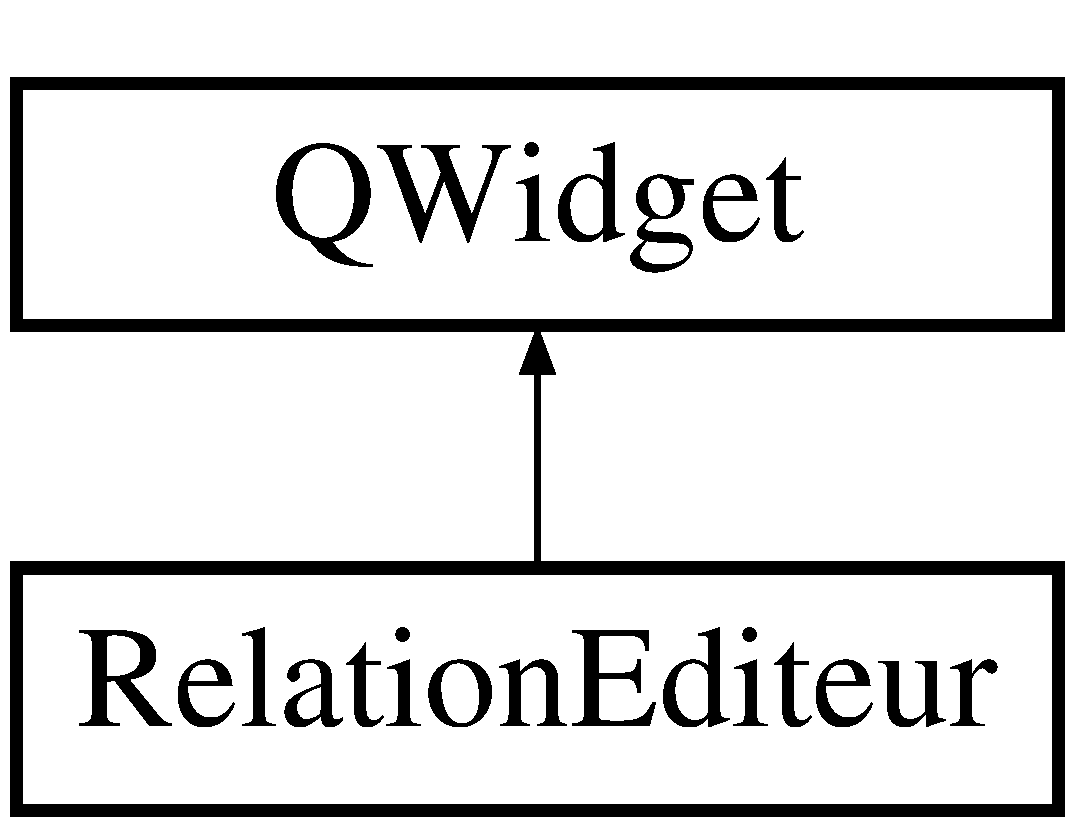
\includegraphics[height=2.000000cm]{class_relation_editeur}
\end{center}
\end{figure}
\subsection*{Connecteurs publics}
\begin{DoxyCompactItemize}
\item 
\hypertarget{class_relation_editeur_a8c46b381f05903282a86411990058b3f}{void \hyperlink{class_relation_editeur_a8c46b381f05903282a86411990058b3f}{save} ()}\label{class_relation_editeur_a8c46b381f05903282a86411990058b3f}

\begin{DoxyCompactList}\small\item\em Enregistre les modifications. \end{DoxyCompactList}\item 
\hypertarget{class_relation_editeur_a0d760d64345d96a887b3002839b79528}{void \hyperlink{class_relation_editeur_a0d760d64345d96a887b3002839b79528}{create} ()}\label{class_relation_editeur_a0d760d64345d96a887b3002839b79528}

\begin{DoxyCompactList}\small\item\em Crée une relation depuis le \hyperlink{class_relation_editeur}{Relation\-Editeur}. \end{DoxyCompactList}\item 
\hypertarget{class_relation_editeur_a4b7de6390f8006db0b0f5b9f50e90ed6}{void \hyperlink{class_relation_editeur_a4b7de6390f8006db0b0f5b9f50e90ed6}{delete\-\_\-relation} ()}\label{class_relation_editeur_a4b7de6390f8006db0b0f5b9f50e90ed6}

\begin{DoxyCompactList}\small\item\em Supprime une relation depuis le \hyperlink{class_relation_editeur}{Relation\-Editeur}. \end{DoxyCompactList}\item 
\hypertarget{class_relation_editeur_aa94f1bdb568c4d7765bead126581e195}{void \hyperlink{class_relation_editeur_aa94f1bdb568c4d7765bead126581e195}{add\-\_\-new\-\_\-couple} ()}\label{class_relation_editeur_aa94f1bdb568c4d7765bead126581e195}

\begin{DoxyCompactList}\small\item\em Création d'un nouveau couple depuis le \hyperlink{class_relation_editeur}{Relation\-Editeur}. \end{DoxyCompactList}\item 
void \hyperlink{class_relation_editeur_a06db7a2ef1338a2aee64c05f4711578c}{set\-\_\-label} (int i)
\begin{DoxyCompactList}\small\item\em Modifie le label d'un couple de la relation. \end{DoxyCompactList}\item 
void \hyperlink{class_relation_editeur_a8af114d6d5e36e71d8ae3f6685ce746a}{remove\-\_\-couple} (int i)
\begin{DoxyCompactList}\small\item\em Supprime un couple de la relation. \end{DoxyCompactList}\end{DoxyCompactItemize}
\subsection*{Signaux}
\begin{DoxyCompactItemize}
\item 
\hypertarget{class_relation_editeur_aa4a4cc9b587d9898ddefa6e7f522f904}{void {\bfseries mon\-Signal} (int)}\label{class_relation_editeur_aa4a4cc9b587d9898ddefa6e7f522f904}

\end{DoxyCompactItemize}
\subsection*{Fonctions membres publiques}
\begin{DoxyCompactItemize}
\item 
\hyperlink{class_relation_editeur_abd28cab2327f3638a00d4e93dcec89fe}{Relation\-Editeur} (\hyperlink{class_relation}{Relation} \&r, Q\-Widget $\ast$parent=0)
\begin{DoxyCompactList}\small\item\em Constructeur (relation existante) \end{DoxyCompactList}\item 
\hypertarget{class_relation_editeur_a18f183e49135d7cf1ecbd809b49d60fc}{\hyperlink{class_relation_editeur_a18f183e49135d7cf1ecbd809b49d60fc}{Relation\-Editeur} (Q\-Widget $\ast$parent=0)}\label{class_relation_editeur_a18f183e49135d7cf1ecbd809b49d60fc}

\begin{DoxyCompactList}\small\item\em Surcharge du constructeur si on souhaite l'afficher \char`\"{}vide\char`\"{} (pour créer une relation) \end{DoxyCompactList}\end{DoxyCompactItemize}
\subsection*{Attributs protégés}
\begin{DoxyCompactItemize}
\item 
\hypertarget{class_relation_editeur_ad3b12fd3a902e575324fbc2485ea0a32}{\hyperlink{class_relation}{Relation} $\ast$ {\bfseries relation}}\label{class_relation_editeur_ad3b12fd3a902e575324fbc2485ea0a32}

\item 
\hypertarget{class_relation_editeur_a84972f3238364a9180f960b69499eabc}{Q\-V\-Box\-Layout $\ast$ {\bfseries layout}}\label{class_relation_editeur_a84972f3238364a9180f960b69499eabc}

\item 
\hypertarget{class_relation_editeur_a386bbf993f724f778c5f2c9a71df0c72}{Q\-Label $\ast$ {\bfseries titre1}}\label{class_relation_editeur_a386bbf993f724f778c5f2c9a71df0c72}

\item 
\hypertarget{class_relation_editeur_a39b2d17ccbc2f9a305f8794fadfbaa31}{Q\-Line\-Edit $\ast$ {\bfseries titre}}\label{class_relation_editeur_a39b2d17ccbc2f9a305f8794fadfbaa31}

\item 
\hypertarget{class_relation_editeur_adf527f7913ba121a81972a895c437e22}{Q\-Label $\ast$ {\bfseries description1}}\label{class_relation_editeur_adf527f7913ba121a81972a895c437e22}

\item 
\hypertarget{class_relation_editeur_a665a987ebabd389767a3224f19194e24}{Q\-Text\-Edit $\ast$ {\bfseries description}}\label{class_relation_editeur_a665a987ebabd389767a3224f19194e24}

\item 
\hypertarget{class_relation_editeur_a66d6d73840a097316b68fb2a0c2f8662}{Q\-Check\-Box $\ast$ {\bfseries orientee}}\label{class_relation_editeur_a66d6d73840a097316b68fb2a0c2f8662}

\item 
\hypertarget{class_relation_editeur_a61a9bd0248797c1be50633743409ebca}{Q\-Push\-Button $\ast$ {\bfseries bouton\-\_\-save}}\label{class_relation_editeur_a61a9bd0248797c1be50633743409ebca}

\item 
\hypertarget{class_relation_editeur_a604e78b34ae17ca57772803044333903}{Q\-Push\-Button $\ast$ {\bfseries bouton\-\_\-delete}}\label{class_relation_editeur_a604e78b34ae17ca57772803044333903}

\item 
\hypertarget{class_relation_editeur_a33cc2dbce2feeab5a6e5b63c1a2fa17e}{Q\-Label $\ast$ {\bfseries couple1}}\label{class_relation_editeur_a33cc2dbce2feeab5a6e5b63c1a2fa17e}

\item 
\hypertarget{class_relation_editeur_a0501d9f22aa7112e0a4c22b20c11ef8a}{Q\-H\-Box\-Layout $\ast$$\ast$ {\bfseries box}}\label{class_relation_editeur_a0501d9f22aa7112e0a4c22b20c11ef8a}

\item 
\hypertarget{class_relation_editeur_a29321b33cf4bd4497997718837586f14}{Q\-Label $\ast$$\ast$ {\bfseries id\-X}}\label{class_relation_editeur_a29321b33cf4bd4497997718837586f14}

\item 
\hypertarget{class_relation_editeur_aea71a6d832c5a279c0fddf344bf3c5fa}{Q\-Label $\ast$$\ast$ {\bfseries id\-Y}}\label{class_relation_editeur_aea71a6d832c5a279c0fddf344bf3c5fa}

\item 
\hypertarget{class_relation_editeur_a90a36570309b063263920e2956dd5530}{Q\-Signal\-Mapper $\ast$ {\bfseries mapper\-\_\-label}}\label{class_relation_editeur_a90a36570309b063263920e2956dd5530}

\item 
\hypertarget{class_relation_editeur_a6bf9deace0be99ee01d29eee5daa4425}{Q\-Line\-Edit $\ast$$\ast$ {\bfseries edit\-\_\-label}}\label{class_relation_editeur_a6bf9deace0be99ee01d29eee5daa4425}

\item 
\hypertarget{class_relation_editeur_aa391b51e4fed9dfee5e1f29ebf7b78b0}{Q\-Push\-Button $\ast$$\ast$ {\bfseries buttons\-\_\-edit}}\label{class_relation_editeur_aa391b51e4fed9dfee5e1f29ebf7b78b0}

\item 
\hypertarget{class_relation_editeur_ad4e996b646c9b4ac74442730fc89b22f}{Q\-Signal\-Mapper $\ast$ {\bfseries mapper\-\_\-remove}}\label{class_relation_editeur_ad4e996b646c9b4ac74442730fc89b22f}

\item 
\hypertarget{class_relation_editeur_ad9856ff6e4193d11ad2b8d6cace478af}{Q\-Push\-Button $\ast$$\ast$ {\bfseries buttons\-\_\-remove}}\label{class_relation_editeur_ad9856ff6e4193d11ad2b8d6cace478af}

\item 
\hypertarget{class_relation_editeur_a51dc2dd05c20a73465ecc69db5355e28}{Q\-H\-Box\-Layout $\ast$ {\bfseries new\-\_\-couple}}\label{class_relation_editeur_a51dc2dd05c20a73465ecc69db5355e28}

\item 
\hypertarget{class_relation_editeur_a7c1d15a6dbf4d0ec867b6a4f9cde7db0}{Q\-Label $\ast$ {\bfseries couple2}}\label{class_relation_editeur_a7c1d15a6dbf4d0ec867b6a4f9cde7db0}

\item 
\hypertarget{class_relation_editeur_a0b925426401fa901808f7720dad0fe35}{Q\-List\-View $\ast$ {\bfseries liste\-\_\-x}}\label{class_relation_editeur_a0b925426401fa901808f7720dad0fe35}

\item 
\hypertarget{class_relation_editeur_ab443cf68744c2b367ea565cc034be39c}{Q\-List\-View $\ast$ {\bfseries liste\-\_\-y}}\label{class_relation_editeur_ab443cf68744c2b367ea565cc034be39c}

\item 
\hypertarget{class_relation_editeur_a3c336e8c1bae8bfd513e1639569cfb19}{Q\-Line\-Edit $\ast$ {\bfseries new\-\_\-label}}\label{class_relation_editeur_a3c336e8c1bae8bfd513e1639569cfb19}

\item 
\hypertarget{class_relation_editeur_ab0c50e29c276fc03fa2a3c5b9fcaa619}{Q\-Push\-Button $\ast$ {\bfseries add\-\_\-couple}}\label{class_relation_editeur_ab0c50e29c276fc03fa2a3c5b9fcaa619}

\item 
\hypertarget{class_relation_editeur_a9b7aad295e2bc9b8c85ec56381914b9f}{Q\-String\-List\-Model $\ast$ {\bfseries model\-\_\-x}}\label{class_relation_editeur_a9b7aad295e2bc9b8c85ec56381914b9f}

\item 
\hypertarget{class_relation_editeur_a747219e4e7bfbe79564ff002bbc81b77}{Q\-String\-List\-Model $\ast$ {\bfseries model\-\_\-y}}\label{class_relation_editeur_a747219e4e7bfbe79564ff002bbc81b77}

\end{DoxyCompactItemize}
\subsection*{Connecteurs privés}
\begin{DoxyCompactItemize}
\item 
\hypertarget{class_relation_editeur_a08f290984e9a90f643f6938a8e1808ff}{void \hyperlink{class_relation_editeur_a08f290984e9a90f643f6938a8e1808ff}{activer\-Bouton} (Q\-String str=\char`\"{}\char`\"{})}\label{class_relation_editeur_a08f290984e9a90f643f6938a8e1808ff}

\begin{DoxyCompactList}\small\item\em Active le bouton \char`\"{}\-Save\char`\"{} quand du texte est modifié. \end{DoxyCompactList}\end{DoxyCompactItemize}


\subsection{Description détaillée}
Permet la visualisation, modification, suppression des relations (interface). 

Classe qui sera par la suite utilisée pour l'ensemble de l'interface (\hyperlink{interface_8h}{interface.\-h}). 

\subsection{Documentation des constructeurs et destructeur}
\hypertarget{class_relation_editeur_abd28cab2327f3638a00d4e93dcec89fe}{\index{Relation\-Editeur@{Relation\-Editeur}!Relation\-Editeur@{Relation\-Editeur}}
\index{Relation\-Editeur@{Relation\-Editeur}!RelationEditeur@{Relation\-Editeur}}
\subsubsection[{Relation\-Editeur}]{\setlength{\rightskip}{0pt plus 5cm}Relation\-Editeur\-::\-Relation\-Editeur (
\begin{DoxyParamCaption}
\item[{{\bf Relation} \&}]{r, }
\item[{Q\-Widget $\ast$}]{parent = {\ttfamily 0}}
\end{DoxyParamCaption}
)\hspace{0.3cm}{\ttfamily [explicit]}}}\label{class_relation_editeur_abd28cab2327f3638a00d4e93dcec89fe}


Constructeur (relation existante) 


\begin{DoxyParams}{Paramètres}
{\em r} & \hyperlink{class_relation}{Relation} à ouvrir \\
\hline
\end{DoxyParams}


\subsection{Documentation des fonctions membres}
\hypertarget{class_relation_editeur_a8af114d6d5e36e71d8ae3f6685ce746a}{\index{Relation\-Editeur@{Relation\-Editeur}!remove\-\_\-couple@{remove\-\_\-couple}}
\index{remove\-\_\-couple@{remove\-\_\-couple}!RelationEditeur@{Relation\-Editeur}}
\subsubsection[{remove\-\_\-couple}]{\setlength{\rightskip}{0pt plus 5cm}void Relation\-Editeur\-::remove\-\_\-couple (
\begin{DoxyParamCaption}
\item[{int}]{i}
\end{DoxyParamCaption}
)\hspace{0.3cm}{\ttfamily [slot]}}}\label{class_relation_editeur_a8af114d6d5e36e71d8ae3f6685ce746a}


Supprime un couple de la relation. 


\begin{DoxyParams}{Paramètres}
{\em i} & indice du couple \\
\hline
\end{DoxyParams}
\hypertarget{class_relation_editeur_a06db7a2ef1338a2aee64c05f4711578c}{\index{Relation\-Editeur@{Relation\-Editeur}!set\-\_\-label@{set\-\_\-label}}
\index{set\-\_\-label@{set\-\_\-label}!RelationEditeur@{Relation\-Editeur}}
\subsubsection[{set\-\_\-label}]{\setlength{\rightskip}{0pt plus 5cm}void Relation\-Editeur\-::set\-\_\-label (
\begin{DoxyParamCaption}
\item[{int}]{i}
\end{DoxyParamCaption}
)\hspace{0.3cm}{\ttfamily [slot]}}}\label{class_relation_editeur_a06db7a2ef1338a2aee64c05f4711578c}


Modifie le label d'un couple de la relation. 


\begin{DoxyParams}{Paramètres}
{\em i} & indice du couple \\
\hline
\end{DoxyParams}


La documentation de cette classe a été générée à partir des fichiers suivants \-:\begin{DoxyCompactItemize}
\item 
/home/camille/\-Documents/\-U\-T\-C/\-H\-U04/\-L\-O21/\-Projet/\-Projet/\hyperlink{relationediteur_8h}{relationediteur.\-h}\item 
/home/camille/\-Documents/\-U\-T\-C/\-H\-U04/\-L\-O21/\-Projet/\-Projet/relationediteur.\-cpp\end{DoxyCompactItemize}

\hypertarget{class_relations_manager}{\section{Référence de la classe Relations\-Manager}
\label{class_relations_manager}\index{Relations\-Manager@{Relations\-Manager}}
}


Permet la gestion de l'ensemble des relations.  




{\ttfamily \#include $<$relation.\-h$>$}

\subsection*{Classes}
\begin{DoxyCompactItemize}
\item 
class \hyperlink{class_relations_manager_1_1_iterator}{Iterator}
\end{DoxyCompactItemize}
\subsection*{Fonctions membres publiques}
\begin{DoxyCompactItemize}
\item 
\hypertarget{class_relations_manager_aad6d18cfe0018bc3c84cd67cc28e02e3}{unsigned int \hyperlink{class_relations_manager_aad6d18cfe0018bc3c84cd67cc28e02e3}{get\-Nb\-Relations} () const }\label{class_relations_manager_aad6d18cfe0018bc3c84cd67cc28e02e3}

\begin{DoxyCompactList}\small\item\em Retourne le nombre de relations du \hyperlink{class_relations_manager}{Relations\-Manager}. \end{DoxyCompactList}\item 
\hyperlink{class_relation}{Relation} \& \hyperlink{class_relations_manager_af3f2992fb1dc52df403ab0213232329d}{get\-I\-Relation} (unsigned int i) const 
\begin{DoxyCompactList}\small\item\em Retourne une relation selon son indice. \end{DoxyCompactList}\item 
\hyperlink{class_relation}{Relation} \& \hyperlink{class_relations_manager_a99ba92089cbce8ab93a1dd16380ead6c}{create\-Relation} (const Q\-String \&titre, const Q\-String \&description, bool is\-Oriente)
\begin{DoxyCompactList}\small\item\em Création d'une nouvelle relation \& ajout au \hyperlink{class_relations_manager}{Relations\-Manager}. \end{DoxyCompactList}\item 
void \hyperlink{class_relations_manager_a48e772342fa842c1832802e6e5e4ee4a}{add\-Relation} (\hyperlink{class_relation}{Relation} \&r)
\begin{DoxyCompactList}\small\item\em Ajout d'une relation existante au \hyperlink{class_relations_manager}{Relations\-Manager}. \end{DoxyCompactList}\item 
void \hyperlink{class_relations_manager_a5929bed08e90a52ec60f3a8cec09766d}{delete\-Relation} (\hyperlink{class_relation}{Relation} \&r)
\begin{DoxyCompactList}\small\item\em Supprime une relation. \end{DoxyCompactList}\item 
\hyperlink{class_relation}{Relation} \& \hyperlink{class_relations_manager_a5d8c2e75d674da855d3b018e2a5ae342}{get\-Relation} (const Q\-String \&titre)
\begin{DoxyCompactList}\small\item\em Permet d'obtenir une relation via son titre. \end{DoxyCompactList}\item 
\hypertarget{class_relations_manager_a6190c96cadd6b056cf94bfb75b5d56d1}{void \hyperlink{class_relations_manager_a6190c96cadd6b056cf94bfb75b5d56d1}{load} ()}\label{class_relations_manager_a6190c96cadd6b056cf94bfb75b5d56d1}

\begin{DoxyCompactList}\small\item\em Permet de charger un fichier de relations. \end{DoxyCompactList}\item 
\hypertarget{class_relations_manager_a8bb101094b5941f53e6d7abe5784ad6e}{void \hyperlink{class_relations_manager_a8bb101094b5941f53e6d7abe5784ad6e}{save} () const }\label{class_relations_manager_a8bb101094b5941f53e6d7abe5784ad6e}

\begin{DoxyCompactList}\small\item\em Permet d'enregistrer les relations dans un fichier. \end{DoxyCompactList}\item 
void \hyperlink{class_relations_manager_a846d7b926b24c57bb3523b582f5a0ea3}{set\-Filename} (const Q\-String \&f)
\begin{DoxyCompactList}\small\item\em Modifie le fichier à ouvrir. \end{DoxyCompactList}\item 
\hypertarget{class_relations_manager_a89cf8af20310718e9608672489683779}{\hyperlink{class_relations_manager_1_1_iterator}{Iterator} \hyperlink{class_relations_manager_a89cf8af20310718e9608672489683779}{get\-Iterator} ()}\label{class_relations_manager_a89cf8af20310718e9608672489683779}

\begin{DoxyCompactList}\small\item\em Permet d'obtenir un iterateur d'un \hyperlink{class_relations_manager}{Relations\-Manager} (D\-P \hyperlink{class_relations_manager_1_1_iterator}{Iterator}) \end{DoxyCompactList}\end{DoxyCompactItemize}
\subsection*{Fonctions membres publiques statiques}
\begin{DoxyCompactItemize}
\item 
static \hyperlink{class_relations_manager}{Relations\-Manager} \& \hyperlink{class_relations_manager_adde192ed5510fc9c4e79a345c42175bc}{get\-Instance} ()
\begin{DoxyCompactList}\small\item\em Retourne l'unique objet \hyperlink{class_relations_manager}{Relations\-Manager} (D\-P Singleton) \end{DoxyCompactList}\end{DoxyCompactItemize}
\subsection*{Fonctions membres privées}
\begin{DoxyCompactItemize}
\item 
\hypertarget{class_relations_manager_a7b9f5d9cd55fa4f51c2c8203f555008a}{\hyperlink{class_relations_manager_a7b9f5d9cd55fa4f51c2c8203f555008a}{Relations\-Manager} ()}\label{class_relations_manager_a7b9f5d9cd55fa4f51c2c8203f555008a}

\begin{DoxyCompactList}\small\item\em Constructeur en privé (D\-P Singleton) \end{DoxyCompactList}\item 
\hypertarget{class_relations_manager_aab9a1490ef70148084c376f94bfca48e}{{\bfseries Relations\-Manager} (const \hyperlink{class_relations_manager}{Relations\-Manager} \&m)}\label{class_relations_manager_aab9a1490ef70148084c376f94bfca48e}

\item 
\hypertarget{class_relations_manager_a44e5d296957404b4553923c3442cfe1b}{\hyperlink{class_relations_manager}{Relations\-Manager} {\bfseries operator=} (const \hyperlink{class_relations_manager}{Relations\-Manager} \&m)}\label{class_relations_manager_a44e5d296957404b4553923c3442cfe1b}

\end{DoxyCompactItemize}
\subsection*{Attributs privés}
\begin{DoxyCompactItemize}
\item 
\hypertarget{class_relations_manager_a99f1b33218d73172bf695c2aec4bec48}{\hyperlink{class_relation}{Relation} $\ast$$\ast$ {\bfseries relations}}\label{class_relations_manager_a99f1b33218d73172bf695c2aec4bec48}

\item 
\hypertarget{class_relations_manager_a2211b0cf547d0ee57bdf0d4bf4fff544}{unsigned int {\bfseries nb\-Relations}}\label{class_relations_manager_a2211b0cf547d0ee57bdf0d4bf4fff544}

\item 
\hypertarget{class_relations_manager_ae710ae31d4f38dac104f52507553fe6c}{unsigned int {\bfseries nb\-Max\-Relations}}\label{class_relations_manager_ae710ae31d4f38dac104f52507553fe6c}

\item 
\hypertarget{class_relations_manager_a3e2c0ce3c9ff25349175dcda0e8623b3}{Q\-String {\bfseries filename}}\label{class_relations_manager_a3e2c0ce3c9ff25349175dcda0e8623b3}

\end{DoxyCompactItemize}


\subsection{Description détaillée}
Permet la gestion de l'ensemble des relations. 

La classe stocke l'ensemble des relations, permet leur modification, suppression, ainsi que la création de nouvelles relations. Toute modification/suppression/création de relation doit obligatoirement passer par le \hyperlink{class_relations_manager}{Relations\-Manager}. 

\subsection{Documentation des fonctions membres}
\hypertarget{class_relations_manager_a48e772342fa842c1832802e6e5e4ee4a}{\index{Relations\-Manager@{Relations\-Manager}!add\-Relation@{add\-Relation}}
\index{add\-Relation@{add\-Relation}!RelationsManager@{Relations\-Manager}}
\subsubsection[{add\-Relation}]{\setlength{\rightskip}{0pt plus 5cm}void Relations\-Manager\-::add\-Relation (
\begin{DoxyParamCaption}
\item[{{\bf Relation} \&}]{r}
\end{DoxyParamCaption}
)}}\label{class_relations_manager_a48e772342fa842c1832802e6e5e4ee4a}


Ajout d'une relation existante au \hyperlink{class_relations_manager}{Relations\-Manager}. 


\begin{DoxyParams}{Paramètres}
{\em r} & \hyperlink{class_relation}{Relation} à ajouter \\
\hline
\end{DoxyParams}
\hypertarget{class_relations_manager_a99ba92089cbce8ab93a1dd16380ead6c}{\index{Relations\-Manager@{Relations\-Manager}!create\-Relation@{create\-Relation}}
\index{create\-Relation@{create\-Relation}!RelationsManager@{Relations\-Manager}}
\subsubsection[{create\-Relation}]{\setlength{\rightskip}{0pt plus 5cm}{\bf Relation} \& Relations\-Manager\-::create\-Relation (
\begin{DoxyParamCaption}
\item[{const Q\-String \&}]{titre, }
\item[{const Q\-String \&}]{description, }
\item[{bool}]{is\-Oriente}
\end{DoxyParamCaption}
)}}\label{class_relations_manager_a99ba92089cbce8ab93a1dd16380ead6c}


Création d'une nouvelle relation \& ajout au \hyperlink{class_relations_manager}{Relations\-Manager}. 


\begin{DoxyParams}{Paramètres}
{\em titre} & Titre \\
\hline
{\em description} & Description \\
\hline
{\em is\-Oriente} & True si la relation est orientée, false sinon \\
\hline
\end{DoxyParams}
\hypertarget{class_relations_manager_a5929bed08e90a52ec60f3a8cec09766d}{\index{Relations\-Manager@{Relations\-Manager}!delete\-Relation@{delete\-Relation}}
\index{delete\-Relation@{delete\-Relation}!RelationsManager@{Relations\-Manager}}
\subsubsection[{delete\-Relation}]{\setlength{\rightskip}{0pt plus 5cm}void Relations\-Manager\-::delete\-Relation (
\begin{DoxyParamCaption}
\item[{{\bf Relation} \&}]{r}
\end{DoxyParamCaption}
)}}\label{class_relations_manager_a5929bed08e90a52ec60f3a8cec09766d}


Supprime une relation. 


\begin{DoxyParams}{Paramètres}
{\em r} & \hyperlink{class_relation}{Relation} à supprimer \\
\hline
\end{DoxyParams}
\hypertarget{class_relations_manager_adde192ed5510fc9c4e79a345c42175bc}{\index{Relations\-Manager@{Relations\-Manager}!get\-Instance@{get\-Instance}}
\index{get\-Instance@{get\-Instance}!RelationsManager@{Relations\-Manager}}
\subsubsection[{get\-Instance}]{\setlength{\rightskip}{0pt plus 5cm}{\bf Relations\-Manager} \& Relations\-Manager\-::get\-Instance (
\begin{DoxyParamCaption}
{}
\end{DoxyParamCaption}
)\hspace{0.3cm}{\ttfamily [static]}}}\label{class_relations_manager_adde192ed5510fc9c4e79a345c42175bc}


Retourne l'unique objet \hyperlink{class_relations_manager}{Relations\-Manager} (D\-P Singleton) 

Crée un \hyperlink{class_relations_manager}{Relations\-Manager} s'il n'en existe pas, renvoie son unique instance sinon. \hypertarget{class_relations_manager_af3f2992fb1dc52df403ab0213232329d}{\index{Relations\-Manager@{Relations\-Manager}!get\-I\-Relation@{get\-I\-Relation}}
\index{get\-I\-Relation@{get\-I\-Relation}!RelationsManager@{Relations\-Manager}}
\subsubsection[{get\-I\-Relation}]{\setlength{\rightskip}{0pt plus 5cm}{\bf Relation}\& Relations\-Manager\-::get\-I\-Relation (
\begin{DoxyParamCaption}
\item[{unsigned int}]{i}
\end{DoxyParamCaption}
) const\hspace{0.3cm}{\ttfamily [inline]}}}\label{class_relations_manager_af3f2992fb1dc52df403ab0213232329d}


Retourne une relation selon son indice. 


\begin{DoxyParams}{Paramètres}
{\em i} & indice de la relation \\
\hline
\end{DoxyParams}
\hypertarget{class_relations_manager_a5d8c2e75d674da855d3b018e2a5ae342}{\index{Relations\-Manager@{Relations\-Manager}!get\-Relation@{get\-Relation}}
\index{get\-Relation@{get\-Relation}!RelationsManager@{Relations\-Manager}}
\subsubsection[{get\-Relation}]{\setlength{\rightskip}{0pt plus 5cm}{\bf Relation} \& Relations\-Manager\-::get\-Relation (
\begin{DoxyParamCaption}
\item[{const Q\-String \&}]{titre}
\end{DoxyParamCaption}
)}}\label{class_relations_manager_a5d8c2e75d674da855d3b018e2a5ae342}


Permet d'obtenir une relation via son titre. 


\begin{DoxyParams}{Paramètres}
{\em titre} & Titre de la relation recherchée \\
\hline
\end{DoxyParams}
\begin{DoxyReturn}{Renvoie}
Une relation 
\end{DoxyReturn}
\hypertarget{class_relations_manager_a846d7b926b24c57bb3523b582f5a0ea3}{\index{Relations\-Manager@{Relations\-Manager}!set\-Filename@{set\-Filename}}
\index{set\-Filename@{set\-Filename}!RelationsManager@{Relations\-Manager}}
\subsubsection[{set\-Filename}]{\setlength{\rightskip}{0pt plus 5cm}void Relations\-Manager\-::set\-Filename (
\begin{DoxyParamCaption}
\item[{const Q\-String \&}]{f}
\end{DoxyParamCaption}
)\hspace{0.3cm}{\ttfamily [inline]}}}\label{class_relations_manager_a846d7b926b24c57bb3523b582f5a0ea3}


Modifie le fichier à ouvrir. 


\begin{DoxyParams}{Paramètres}
{\em f} & Chemin du fichier à ouvrir \\
\hline
\end{DoxyParams}


La documentation de cette classe a été générée à partir des fichiers suivants \-:\begin{DoxyCompactItemize}
\item 
/home/camille/\-Documents/\-U\-T\-C/\-H\-U04/\-L\-O21/\-Projet/\-Projet/\hyperlink{relation_8h}{relation.\-h}\item 
/home/camille/\-Documents/\-U\-T\-C/\-H\-U04/\-L\-O21/\-Projet/\-Projet/\hyperlink{relation_8cpp}{relation.\-cpp}\end{DoxyCompactItemize}

\hypertarget{class_tache}{\section{Référence de la classe Tache}
\label{class_tache}\index{Tache@{Tache}}
}


Représente une tâche, sans deadline ni priorité.  




{\ttfamily \#include $<$note.\-h$>$}

Graphe d'héritage de Tache\-:\begin{figure}[H]
\begin{center}
\leavevmode
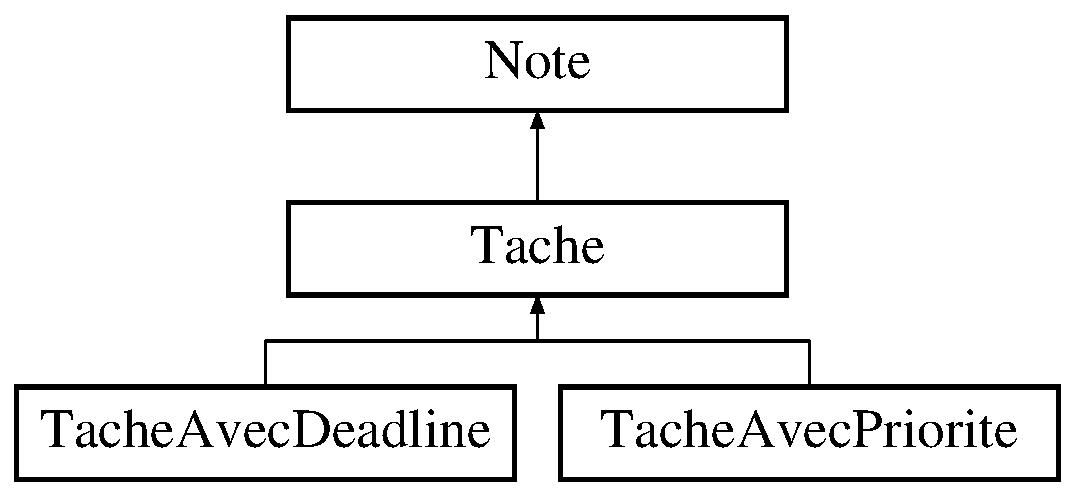
\includegraphics[height=3.000000cm]{class_tache}
\end{center}
\end{figure}
\subsection*{Fonctions membres publiques}
\begin{DoxyCompactItemize}
\item 
Q\-String \hyperlink{class_tache_add34adcc7d4fb26078afaae3b92bdd76}{get\-Texte} () const 
\begin{DoxyCompactList}\small\item\em get\-Texte \end{DoxyCompactList}\item 
Tache\-Statut \hyperlink{class_tache_a9507985ede212921bdc47c722d2e56b1}{get\-Statut} () const 
\begin{DoxyCompactList}\small\item\em get\-Statut \end{DoxyCompactList}\end{DoxyCompactItemize}
\subsection*{Fonctions membres protégées}
\begin{DoxyCompactItemize}
\item 
\hyperlink{class_tache_a2c7f6baff58554458a0cf3edb28a24c4}{Tache} (Q\-String id, Q\-String t, Q\-String text, Q\-Date date\-\_\-c=Q\-Date\-::current\-Date(), Q\-Date date\-\_\-m=Q\-Date\-::current\-Date(), bool last=true, int v=1, Note\-Etat e=active, Tache\-Statut st=attente)
\begin{DoxyCompactList}\small\item\em Constructeur d'une tâche sans deadline ni priorité \end{DoxyCompactList}\end{DoxyCompactItemize}
\subsection*{Attributs protégés}
\begin{DoxyCompactItemize}
\item 
\hypertarget{class_tache_a0854b4630c361484c1d4f0b154de5168}{Q\-String {\bfseries texte}}\label{class_tache_a0854b4630c361484c1d4f0b154de5168}

\item 
\hypertarget{class_tache_a270d72fa7d91f115cca5d5cb14e8eea6}{Tache\-Statut {\bfseries statut}}\label{class_tache_a270d72fa7d91f115cca5d5cb14e8eea6}

\end{DoxyCompactItemize}
\subsection*{Amis}
\begin{DoxyCompactItemize}
\item 
\hypertarget{class_tache_a017a5144e8cfa6087305055ab968ef41}{class {\bfseries Notes\-Manager}}\label{class_tache_a017a5144e8cfa6087305055ab968ef41}

\end{DoxyCompactItemize}


\subsection{Description détaillée}
Représente une tâche, sans deadline ni priorité. 

\subsection{Documentation des constructeurs et destructeur}
\hypertarget{class_tache_a2c7f6baff58554458a0cf3edb28a24c4}{\index{Tache@{Tache}!Tache@{Tache}}
\index{Tache@{Tache}!Tache@{Tache}}
\subsubsection[{Tache}]{\setlength{\rightskip}{0pt plus 5cm}Tache\-::\-Tache (
\begin{DoxyParamCaption}
\item[{Q\-String}]{id, }
\item[{Q\-String}]{t, }
\item[{Q\-String}]{text, }
\item[{Q\-Date}]{date\-\_\-c = {\ttfamily QDate\-:\-:currentDate()}, }
\item[{Q\-Date}]{date\-\_\-m = {\ttfamily QDate\-:\-:currentDate()}, }
\item[{bool}]{last = {\ttfamily true}, }
\item[{int}]{v = {\ttfamily 1}, }
\item[{Note\-Etat}]{e = {\ttfamily active}, }
\item[{Tache\-Statut}]{st = {\ttfamily attente}}
\end{DoxyParamCaption}
)\hspace{0.3cm}{\ttfamily [inline]}, {\ttfamily [protected]}}}\label{class_tache_a2c7f6baff58554458a0cf3edb28a24c4}


Constructeur d'une tâche sans deadline ni priorité 


\begin{DoxyParams}{Paramètres}
{\em id} & L'identificateur de la note \\
\hline
{\em t} & Le titre de la note \\
\hline
{\em date\-\_\-c} & La date de création \\
\hline
{\em date\-\_\-m} & La date de dernière modification \\
\hline
{\em last} & Indique si c'est la dernière version de la note ou pas \\
\hline
{\em v} & Version de la note \\
\hline
{\em e} & Etat de la note (active, archivée ou corbeille). \\
\hline
{\em text} & Contenu de la tâche \\
\hline
{\em st} & Le statut (attente, cours, terminee) \\
\hline
\end{DoxyParams}


\subsection{Documentation des fonctions membres}
\hypertarget{class_tache_a9507985ede212921bdc47c722d2e56b1}{\index{Tache@{Tache}!get\-Statut@{get\-Statut}}
\index{get\-Statut@{get\-Statut}!Tache@{Tache}}
\subsubsection[{get\-Statut}]{\setlength{\rightskip}{0pt plus 5cm}Tache\-Statut Tache\-::get\-Statut (
\begin{DoxyParamCaption}
{}
\end{DoxyParamCaption}
) const\hspace{0.3cm}{\ttfamily [inline]}}}\label{class_tache_a9507985ede212921bdc47c722d2e56b1}


get\-Statut 

\begin{DoxyReturn}{Renvoie}
Retourne le statut de la tâche. 
\end{DoxyReturn}
\hypertarget{class_tache_add34adcc7d4fb26078afaae3b92bdd76}{\index{Tache@{Tache}!get\-Texte@{get\-Texte}}
\index{get\-Texte@{get\-Texte}!Tache@{Tache}}
\subsubsection[{get\-Texte}]{\setlength{\rightskip}{0pt plus 5cm}Q\-String Tache\-::get\-Texte (
\begin{DoxyParamCaption}
{}
\end{DoxyParamCaption}
) const\hspace{0.3cm}{\ttfamily [inline]}}}\label{class_tache_add34adcc7d4fb26078afaae3b92bdd76}


get\-Texte 

\begin{DoxyReturn}{Renvoie}
Retourne le contenu de la tâche. 
\end{DoxyReturn}


La documentation de cette classe a été générée à partir des fichiers suivants \-:\begin{DoxyCompactItemize}
\item 
/home/camille/\-Documents/\-U\-T\-C/\-H\-U04/\-L\-O21/\-Projet/\-Projet/\hyperlink{note_8h}{note.\-h}\item 
/home/camille/\-Documents/\-U\-T\-C/\-H\-U04/\-L\-O21/\-Projet/\-Projet/\hyperlink{note_8cpp}{note.\-cpp}\end{DoxyCompactItemize}

\hypertarget{class_tache_avec_deadline}{\section{Référence de la classe Tache\-Avec\-Deadline}
\label{class_tache_avec_deadline}\index{Tache\-Avec\-Deadline@{Tache\-Avec\-Deadline}}
}


Représente une tâche avec deadline.  




{\ttfamily \#include $<$note.\-h$>$}

Graphe d'héritage de Tache\-Avec\-Deadline\-:\begin{figure}[H]
\begin{center}
\leavevmode
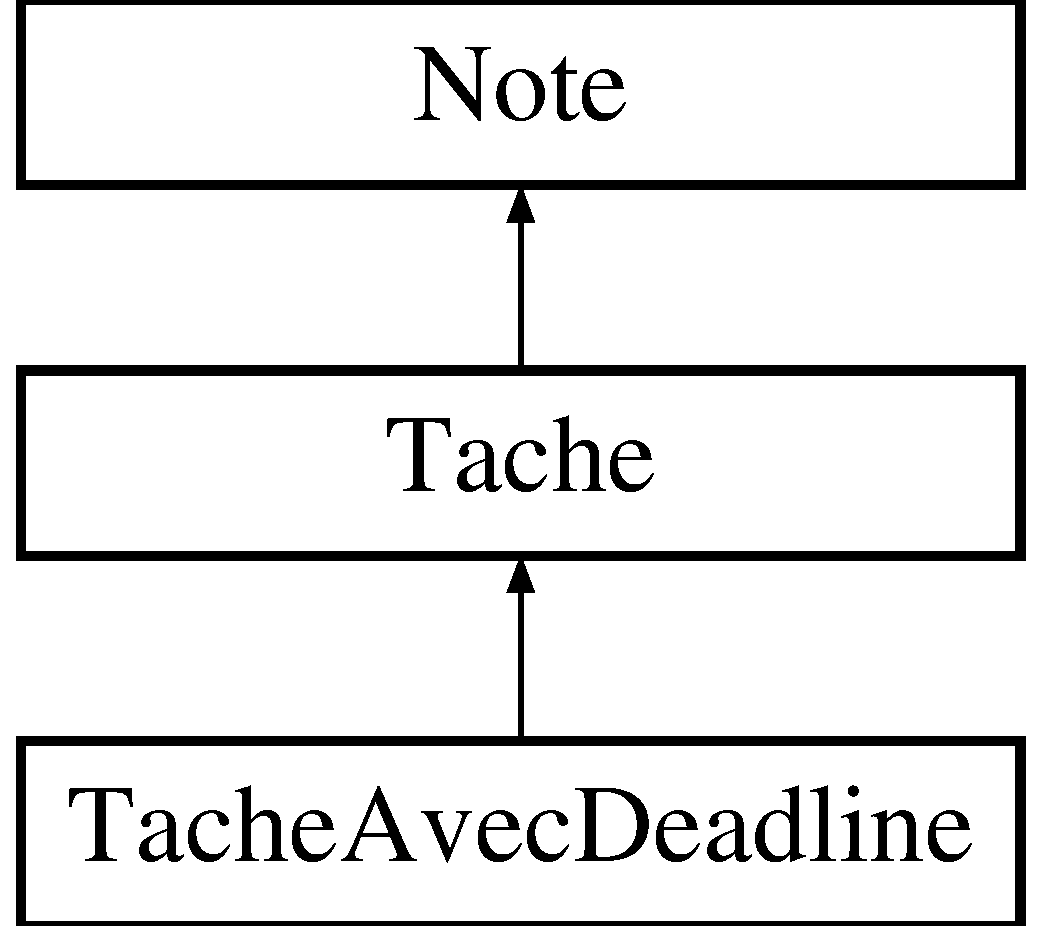
\includegraphics[height=3.000000cm]{class_tache_avec_deadline}
\end{center}
\end{figure}
\subsection*{Fonctions membres publiques}
\begin{DoxyCompactItemize}
\item 
Q\-Date \hyperlink{class_tache_avec_deadline_a108926cb0f3aeb527f952faa34a5a81a}{get\-Deadline} () const 
\begin{DoxyCompactList}\small\item\em get\-Deadline \end{DoxyCompactList}\end{DoxyCompactItemize}
\subsection*{Fonctions membres protégées}
\begin{DoxyCompactItemize}
\item 
\hyperlink{class_tache_avec_deadline_aa8b2ac4efce7571174313a6396e4d4bd}{Tache\-Avec\-Deadline} (Q\-String id, Q\-String t, Q\-String text, Q\-Date dead, Q\-Date date\-\_\-c=Q\-Date\-::current\-Date(), Q\-Date date\-\_\-m=Q\-Date\-::current\-Date(), bool last=true, int v=1, Note\-Etat e=active, Tache\-Statut st=attente)
\begin{DoxyCompactList}\small\item\em Constructeur d'une tâche avec deadline. \end{DoxyCompactList}\end{DoxyCompactItemize}
\subsection*{Attributs protégés}
\begin{DoxyCompactItemize}
\item 
\hypertarget{class_tache_avec_deadline_a87c17be01a41bc30d625a68faecd25b2}{Q\-Date {\bfseries deadline}}\label{class_tache_avec_deadline_a87c17be01a41bc30d625a68faecd25b2}

\end{DoxyCompactItemize}
\subsection*{Amis}
\begin{DoxyCompactItemize}
\item 
\hypertarget{class_tache_avec_deadline_a017a5144e8cfa6087305055ab968ef41}{class {\bfseries Notes\-Manager}}\label{class_tache_avec_deadline_a017a5144e8cfa6087305055ab968ef41}

\end{DoxyCompactItemize}


\subsection{Description détaillée}
Représente une tâche avec deadline. 

\subsection{Documentation des constructeurs et destructeur}
\hypertarget{class_tache_avec_deadline_aa8b2ac4efce7571174313a6396e4d4bd}{\index{Tache\-Avec\-Deadline@{Tache\-Avec\-Deadline}!Tache\-Avec\-Deadline@{Tache\-Avec\-Deadline}}
\index{Tache\-Avec\-Deadline@{Tache\-Avec\-Deadline}!TacheAvecDeadline@{Tache\-Avec\-Deadline}}
\subsubsection[{Tache\-Avec\-Deadline}]{\setlength{\rightskip}{0pt plus 5cm}Tache\-Avec\-Deadline\-::\-Tache\-Avec\-Deadline (
\begin{DoxyParamCaption}
\item[{Q\-String}]{id, }
\item[{Q\-String}]{t, }
\item[{Q\-String}]{text, }
\item[{Q\-Date}]{dead, }
\item[{Q\-Date}]{date\-\_\-c = {\ttfamily QDate\-:\-:currentDate()}, }
\item[{Q\-Date}]{date\-\_\-m = {\ttfamily QDate\-:\-:currentDate()}, }
\item[{bool}]{last = {\ttfamily true}, }
\item[{int}]{v = {\ttfamily 1}, }
\item[{Note\-Etat}]{e = {\ttfamily active}, }
\item[{Tache\-Statut}]{st = {\ttfamily attente}}
\end{DoxyParamCaption}
)\hspace{0.3cm}{\ttfamily [inline]}, {\ttfamily [protected]}}}\label{class_tache_avec_deadline_aa8b2ac4efce7571174313a6396e4d4bd}


Constructeur d'une tâche avec deadline. 


\begin{DoxyParams}{Paramètres}
{\em id} & L'identificateur de la note \\
\hline
{\em t} & Le titre de la note \\
\hline
{\em date\-\_\-c} & La date de création \\
\hline
{\em date\-\_\-m} & La date de dernière modification \\
\hline
{\em last} & Indique si c'est la dernière version de la note ou pas \\
\hline
{\em v} & Version de la note \\
\hline
{\em e} & Etat de la note (active, archivée ou corbeille). \\
\hline
{\em text} & Contenu de la tâche \\
\hline
{\em st} & Le statut (attente, cours, terminee) \\
\hline
{\em dead} & La deadline \\
\hline
\end{DoxyParams}


\subsection{Documentation des fonctions membres}
\hypertarget{class_tache_avec_deadline_a108926cb0f3aeb527f952faa34a5a81a}{\index{Tache\-Avec\-Deadline@{Tache\-Avec\-Deadline}!get\-Deadline@{get\-Deadline}}
\index{get\-Deadline@{get\-Deadline}!TacheAvecDeadline@{Tache\-Avec\-Deadline}}
\subsubsection[{get\-Deadline}]{\setlength{\rightskip}{0pt plus 5cm}Q\-Date Tache\-Avec\-Deadline\-::get\-Deadline (
\begin{DoxyParamCaption}
{}
\end{DoxyParamCaption}
) const\hspace{0.3cm}{\ttfamily [inline]}}}\label{class_tache_avec_deadline_a108926cb0f3aeb527f952faa34a5a81a}


get\-Deadline 

\begin{DoxyReturn}{Renvoie}
La deadline de la tâche. 
\end{DoxyReturn}


La documentation de cette classe a été générée à partir des fichiers suivants \-:\begin{DoxyCompactItemize}
\item 
/home/camille/\-Documents/\-U\-T\-C/\-H\-U04/\-L\-O21/\-Projet/\-Projet/\hyperlink{note_8h}{note.\-h}\item 
/home/camille/\-Documents/\-U\-T\-C/\-H\-U04/\-L\-O21/\-Projet/\-Projet/\hyperlink{note_8cpp}{note.\-cpp}\end{DoxyCompactItemize}

\hypertarget{class_tache_avec_deadline_editeur}{\section{Référence de la classe Tache\-Avec\-Deadline\-Editeur}
\label{class_tache_avec_deadline_editeur}\index{Tache\-Avec\-Deadline\-Editeur@{Tache\-Avec\-Deadline\-Editeur}}
}


Permet de visualiser et modifier les tâches avec deadline (interface).  




{\ttfamily \#include $<$noteediteur.\-h$>$}

Graphe d'héritage de Tache\-Avec\-Deadline\-Editeur\-:\begin{figure}[H]
\begin{center}
\leavevmode
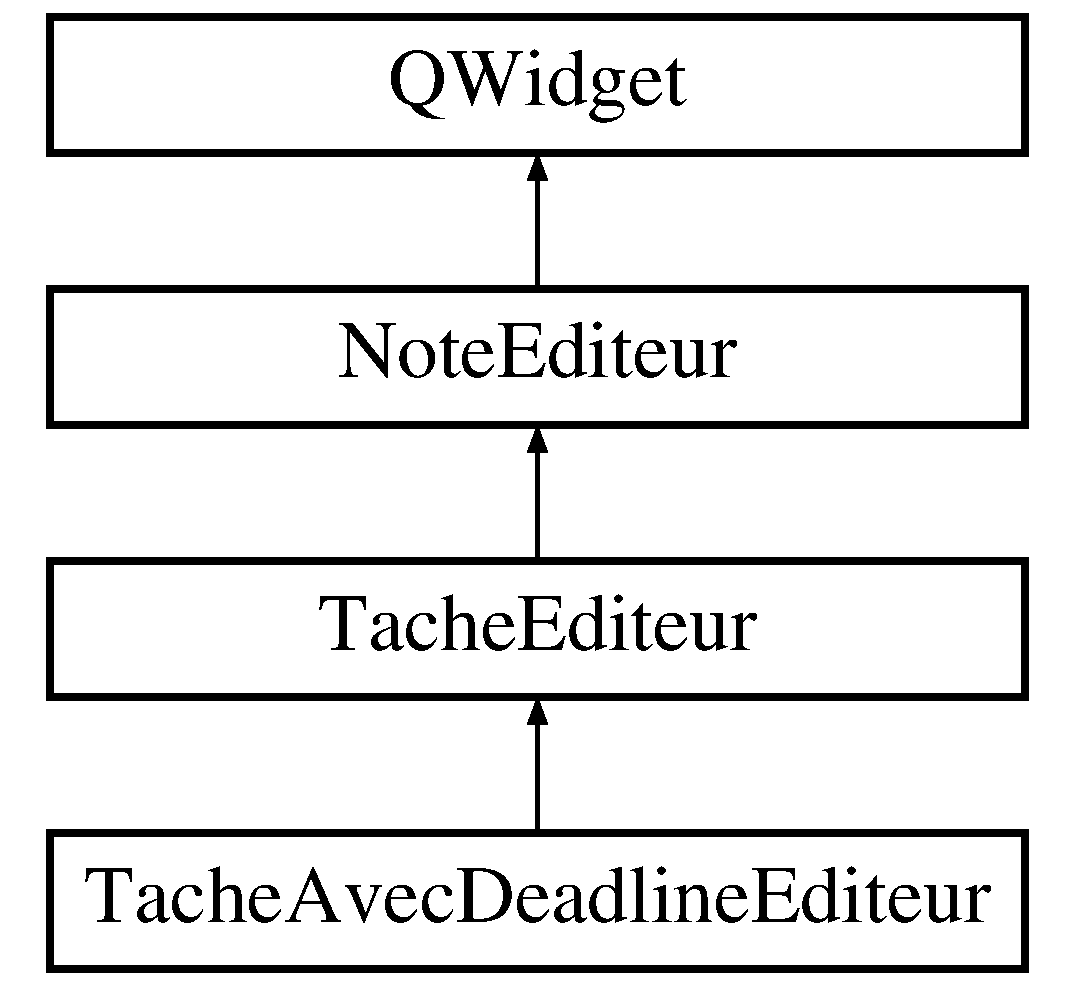
\includegraphics[height=4.000000cm]{class_tache_avec_deadline_editeur}
\end{center}
\end{figure}
\subsection*{Connecteurs publics}
\begin{DoxyCompactItemize}
\item 
\hypertarget{class_tache_avec_deadline_editeur_adba63da747f669eb68f1933fb0c442b2}{void \hyperlink{class_tache_avec_deadline_editeur_adba63da747f669eb68f1933fb0c442b2}{extensionsave} ()}\label{class_tache_avec_deadline_editeur_adba63da747f669eb68f1933fb0c442b2}

\begin{DoxyCompactList}\small\item\em Définit la sauvegarde selon la sous-\/classe de note (appelée par \hyperlink{class_note_editeur_a605b1bca885c25460cb7d8863d1f3d03}{save()}) \end{DoxyCompactList}\item 
\hypertarget{class_tache_avec_deadline_editeur_a65604ab58431d7c791e6b39ea005a5ab}{void \hyperlink{class_tache_avec_deadline_editeur_a65604ab58431d7c791e6b39ea005a5ab}{extensionsetasactual} ()}\label{class_tache_avec_deadline_editeur_a65604ab58431d7c791e6b39ea005a5ab}

\begin{DoxyCompactList}\small\item\em Définit l'actualisation selon la sous-\/classe de la note (appelée par \hyperlink{class_note_editeur_a857f285628a0b7dcb6a69b18c977aa71}{set\-As\-Actual()}) \end{DoxyCompactList}\item 
\hypertarget{class_tache_avec_deadline_editeur_a4a72b30f20d2059f38ba72376e94437e}{void \hyperlink{class_tache_avec_deadline_editeur_a4a72b30f20d2059f38ba72376e94437e}{create} ()}\label{class_tache_avec_deadline_editeur_a4a72b30f20d2059f38ba72376e94437e}

\begin{DoxyCompactList}\small\item\em Création d'un nouvel objet tache\-Avec\-Deadline depuis l'tache\-Avec\-Deadline\-Editeur. \end{DoxyCompactList}\end{DoxyCompactItemize}
\subsection*{Fonctions membres publiques}
\begin{DoxyCompactItemize}
\item 
\hyperlink{class_tache_avec_deadline_editeur_aa56d0511ae2f2ca9ae20881df4852ed5}{Tache\-Avec\-Deadline\-Editeur} (\hyperlink{class_tache_avec_deadline}{Tache\-Avec\-Deadline} \&t, Q\-Widget $\ast$parent=0)
\begin{DoxyCompactList}\small\item\em Constructeur. \end{DoxyCompactList}\item 
\hypertarget{class_tache_avec_deadline_editeur_ab851241684748660a8eb640e176539e0}{\hyperlink{class_tache_avec_deadline_editeur_ab851241684748660a8eb640e176539e0}{Tache\-Avec\-Deadline\-Editeur} (Q\-Widget $\ast$parent=0)}\label{class_tache_avec_deadline_editeur_ab851241684748660a8eb640e176539e0}

\begin{DoxyCompactList}\small\item\em Surcharge de constructeur si on n'a pas de tâche à afficher. \end{DoxyCompactList}\item 
\hypertarget{class_tache_avec_deadline_editeur_a6846c1e2cb58616ee11906fec57374ad}{void \hyperlink{class_tache_avec_deadline_editeur_a6846c1e2cb58616ee11906fec57374ad}{blockall} ()}\label{class_tache_avec_deadline_editeur_a6846c1e2cb58616ee11906fec57374ad}

\begin{DoxyCompactList}\small\item\em Permet d'interdire toute action à l'utilisateur (désactive tous les boutons) \end{DoxyCompactList}\end{DoxyCompactItemize}
\subsection*{Attributs protégés}
\begin{DoxyCompactItemize}
\item 
\hypertarget{class_tache_avec_deadline_editeur_a350f2f88b99289cef5d815a855364718}{Q\-Label $\ast$ {\bfseries deadline1}}\label{class_tache_avec_deadline_editeur_a350f2f88b99289cef5d815a855364718}

\item 
\hypertarget{class_tache_avec_deadline_editeur_ab5299170c8c8cd9fa705e1c6d28fc607}{Q\-Date\-Edit $\ast$ {\bfseries deadline}}\label{class_tache_avec_deadline_editeur_ab5299170c8c8cd9fa705e1c6d28fc607}

\end{DoxyCompactItemize}


\subsection{Description détaillée}
Permet de visualiser et modifier les tâches avec deadline (interface). 

Classe qui est par la suite utilisée pour réaliser l'ensemble de l'interface graphiue (\hyperlink{interface_8h}{interface.\-h}). 

\subsection{Documentation des constructeurs et destructeur}
\hypertarget{class_tache_avec_deadline_editeur_aa56d0511ae2f2ca9ae20881df4852ed5}{\index{Tache\-Avec\-Deadline\-Editeur@{Tache\-Avec\-Deadline\-Editeur}!Tache\-Avec\-Deadline\-Editeur@{Tache\-Avec\-Deadline\-Editeur}}
\index{Tache\-Avec\-Deadline\-Editeur@{Tache\-Avec\-Deadline\-Editeur}!TacheAvecDeadlineEditeur@{Tache\-Avec\-Deadline\-Editeur}}
\subsubsection[{Tache\-Avec\-Deadline\-Editeur}]{\setlength{\rightskip}{0pt plus 5cm}Tache\-Avec\-Deadline\-Editeur\-::\-Tache\-Avec\-Deadline\-Editeur (
\begin{DoxyParamCaption}
\item[{{\bf Tache\-Avec\-Deadline} \&}]{t, }
\item[{Q\-Widget $\ast$}]{parent = {\ttfamily 0}}
\end{DoxyParamCaption}
)}}\label{class_tache_avec_deadline_editeur_aa56d0511ae2f2ca9ae20881df4852ed5}


Constructeur. 


\begin{DoxyParams}{Paramètres}
{\em t} & Tâche à afficher \\
\hline
\end{DoxyParams}


La documentation de cette classe a été générée à partir des fichiers suivants \-:\begin{DoxyCompactItemize}
\item 
/home/camille/\-Documents/\-U\-T\-C/\-H\-U04/\-L\-O21/\-Projet/\-Projet/\hyperlink{noteediteur_8h}{noteediteur.\-h}\item 
/home/camille/\-Documents/\-U\-T\-C/\-H\-U04/\-L\-O21/\-Projet/\-Projet/noteediteur.\-cpp\end{DoxyCompactItemize}

\hypertarget{class_tache_avec_priorite}{\section{Référence de la classe Tache\-Avec\-Priorite}
\label{class_tache_avec_priorite}\index{Tache\-Avec\-Priorite@{Tache\-Avec\-Priorite}}
}


Représente une tâche avec priorité  




{\ttfamily \#include $<$note.\-h$>$}

Graphe d'héritage de Tache\-Avec\-Priorite\-:\begin{figure}[H]
\begin{center}
\leavevmode
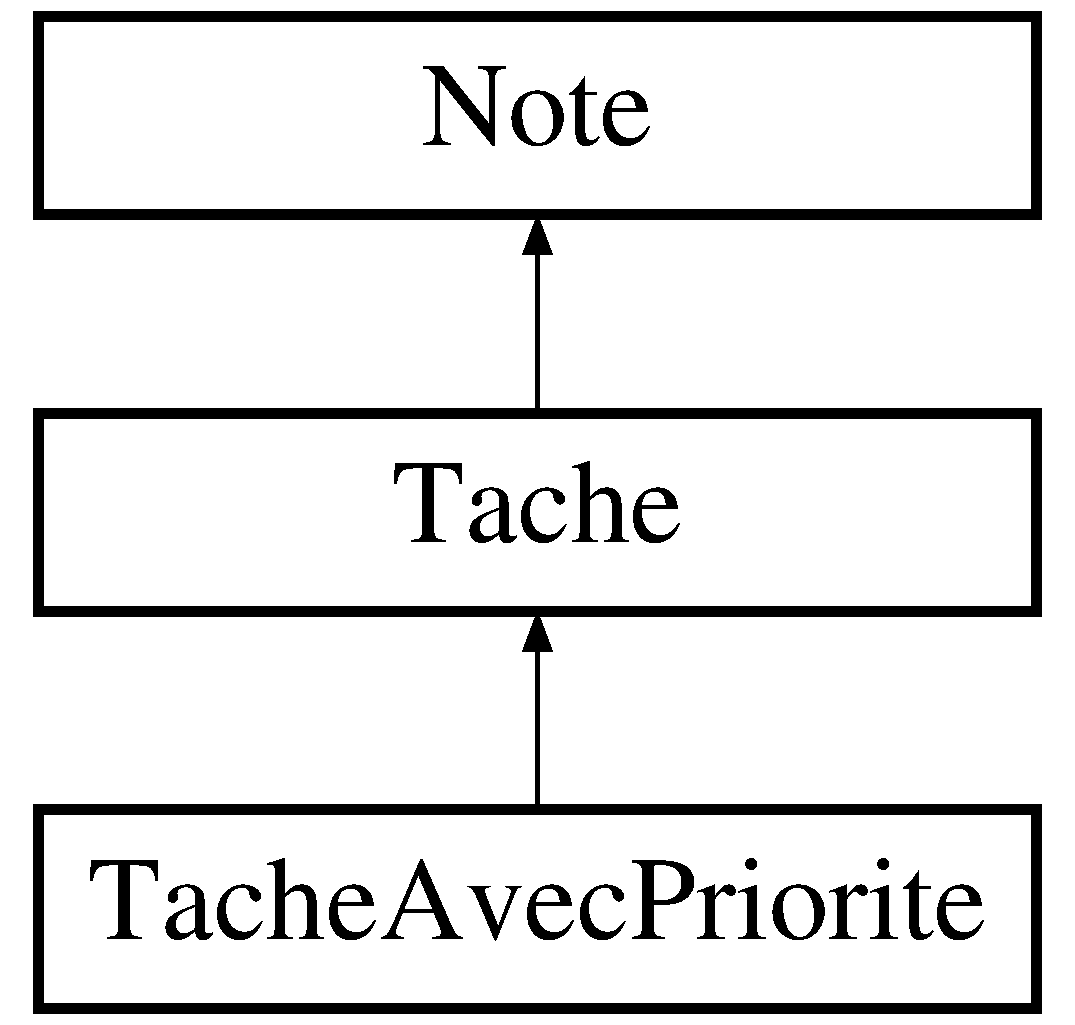
\includegraphics[height=3.000000cm]{class_tache_avec_priorite}
\end{center}
\end{figure}
\subsection*{Fonctions membres publiques}
\begin{DoxyCompactItemize}
\item 
int \hyperlink{class_tache_avec_priorite_ab932dc1d71765a1e124d2a398248ee6c}{get\-Priorite} () const 
\begin{DoxyCompactList}\small\item\em get\-Priorite \end{DoxyCompactList}\end{DoxyCompactItemize}
\subsection*{Fonctions membres protégées}
\begin{DoxyCompactItemize}
\item 
\hyperlink{class_tache_avec_priorite_a4ef6dcacb0c6837227fae4e96718a40b}{Tache\-Avec\-Priorite} (Q\-String id, Q\-String t, Q\-String text, Q\-Date date\-\_\-c=Q\-Date\-::current\-Date(), Q\-Date date\-\_\-m=Q\-Date\-::current\-Date(), bool last=true, int v=1, Note\-Etat e=active, Tache\-Statut st=attente, int p=0)
\begin{DoxyCompactList}\small\item\em Constructeur d'une tâche avec priorité \end{DoxyCompactList}\end{DoxyCompactItemize}
\subsection*{Attributs protégés}
\begin{DoxyCompactItemize}
\item 
\hypertarget{class_tache_avec_priorite_a812663c068df76d7a8f4c1d486b25262}{unsigned int {\bfseries priorite}}\label{class_tache_avec_priorite_a812663c068df76d7a8f4c1d486b25262}

\end{DoxyCompactItemize}
\subsection*{Amis}
\begin{DoxyCompactItemize}
\item 
\hypertarget{class_tache_avec_priorite_a017a5144e8cfa6087305055ab968ef41}{class {\bfseries Notes\-Manager}}\label{class_tache_avec_priorite_a017a5144e8cfa6087305055ab968ef41}

\end{DoxyCompactItemize}


\subsection{Description détaillée}
Représente une tâche avec priorité 

\subsection{Documentation des constructeurs et destructeur}
\hypertarget{class_tache_avec_priorite_a4ef6dcacb0c6837227fae4e96718a40b}{\index{Tache\-Avec\-Priorite@{Tache\-Avec\-Priorite}!Tache\-Avec\-Priorite@{Tache\-Avec\-Priorite}}
\index{Tache\-Avec\-Priorite@{Tache\-Avec\-Priorite}!TacheAvecPriorite@{Tache\-Avec\-Priorite}}
\subsubsection[{Tache\-Avec\-Priorite}]{\setlength{\rightskip}{0pt plus 5cm}Tache\-Avec\-Priorite\-::\-Tache\-Avec\-Priorite (
\begin{DoxyParamCaption}
\item[{Q\-String}]{id, }
\item[{Q\-String}]{t, }
\item[{Q\-String}]{text, }
\item[{Q\-Date}]{date\-\_\-c = {\ttfamily QDate\-:\-:currentDate()}, }
\item[{Q\-Date}]{date\-\_\-m = {\ttfamily QDate\-:\-:currentDate()}, }
\item[{bool}]{last = {\ttfamily true}, }
\item[{int}]{v = {\ttfamily 1}, }
\item[{Note\-Etat}]{e = {\ttfamily active}, }
\item[{Tache\-Statut}]{st = {\ttfamily attente}, }
\item[{int}]{p = {\ttfamily 0}}
\end{DoxyParamCaption}
)\hspace{0.3cm}{\ttfamily [inline]}, {\ttfamily [protected]}}}\label{class_tache_avec_priorite_a4ef6dcacb0c6837227fae4e96718a40b}


Constructeur d'une tâche avec priorité 


\begin{DoxyParams}{Paramètres}
{\em id} & L'identificateur de la note \\
\hline
{\em t} & Le titre de la note \\
\hline
{\em date\-\_\-c} & La date de création \\
\hline
{\em date\-\_\-m} & La date de dernière modification \\
\hline
{\em last} & Indique si c'est la dernière version de la note ou pas \\
\hline
{\em v} & Version de la note \\
\hline
{\em e} & Etat de la note (active, archivée ou corbeille). \\
\hline
{\em text} & Contenu de la tâche \\
\hline
{\em st} & Le statut (attente, cours, terminee) \\
\hline
{\em p} & La priorité \\
\hline
\end{DoxyParams}


\subsection{Documentation des fonctions membres}
\hypertarget{class_tache_avec_priorite_ab932dc1d71765a1e124d2a398248ee6c}{\index{Tache\-Avec\-Priorite@{Tache\-Avec\-Priorite}!get\-Priorite@{get\-Priorite}}
\index{get\-Priorite@{get\-Priorite}!TacheAvecPriorite@{Tache\-Avec\-Priorite}}
\subsubsection[{get\-Priorite}]{\setlength{\rightskip}{0pt plus 5cm}int Tache\-Avec\-Priorite\-::get\-Priorite (
\begin{DoxyParamCaption}
{}
\end{DoxyParamCaption}
) const\hspace{0.3cm}{\ttfamily [inline]}}}\label{class_tache_avec_priorite_ab932dc1d71765a1e124d2a398248ee6c}


get\-Priorite 

\begin{DoxyReturn}{Renvoie}
La priorité 
\end{DoxyReturn}


La documentation de cette classe a été générée à partir des fichiers suivants \-:\begin{DoxyCompactItemize}
\item 
/home/camille/\-Documents/\-U\-T\-C/\-H\-U04/\-L\-O21/\-Projet/\-Projet/\hyperlink{note_8h}{note.\-h}\item 
/home/camille/\-Documents/\-U\-T\-C/\-H\-U04/\-L\-O21/\-Projet/\-Projet/\hyperlink{note_8cpp}{note.\-cpp}\end{DoxyCompactItemize}

\hypertarget{class_tache_avec_priorite_editeur}{\section{Référence de la classe Tache\-Avec\-Priorite\-Editeur}
\label{class_tache_avec_priorite_editeur}\index{Tache\-Avec\-Priorite\-Editeur@{Tache\-Avec\-Priorite\-Editeur}}
}


Permet de visualiser et modifier les tâches avec priorité (interface).  




{\ttfamily \#include $<$noteediteur.\-h$>$}

Graphe d'héritage de Tache\-Avec\-Priorite\-Editeur\-:\begin{figure}[H]
\begin{center}
\leavevmode
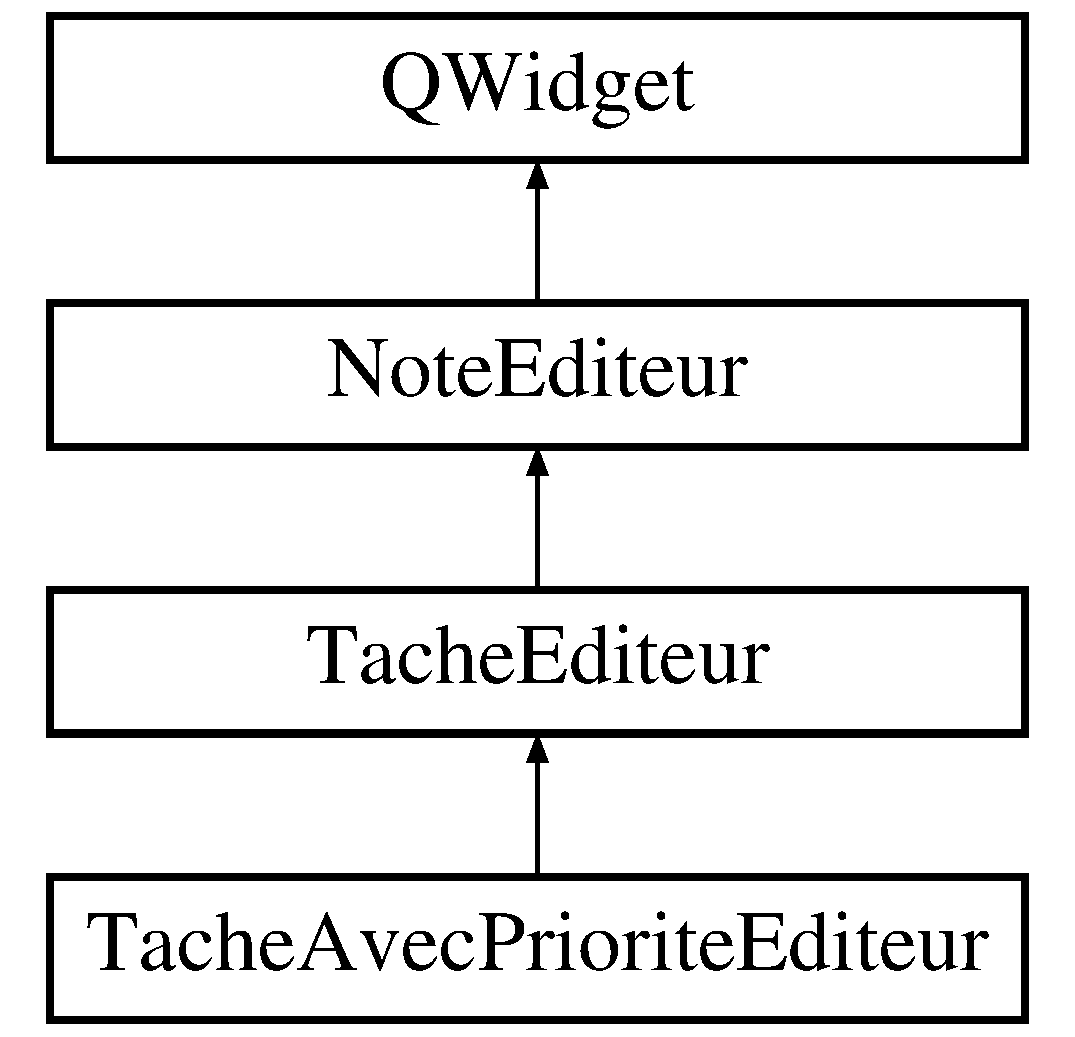
\includegraphics[height=4.000000cm]{class_tache_avec_priorite_editeur}
\end{center}
\end{figure}
\subsection*{Connecteurs publics}
\begin{DoxyCompactItemize}
\item 
\hypertarget{class_tache_avec_priorite_editeur_a46fbeac1f204d539c7690fc1e523e53a}{void \hyperlink{class_tache_avec_priorite_editeur_a46fbeac1f204d539c7690fc1e523e53a}{extensionsave} ()}\label{class_tache_avec_priorite_editeur_a46fbeac1f204d539c7690fc1e523e53a}

\begin{DoxyCompactList}\small\item\em Définit la sauvegarde selon la sous-\/classe de note (appelée par \hyperlink{class_note_editeur_a605b1bca885c25460cb7d8863d1f3d03}{save()}) \end{DoxyCompactList}\item 
\hypertarget{class_tache_avec_priorite_editeur_a964d98a080a52565eea17d24db923b1e}{void \hyperlink{class_tache_avec_priorite_editeur_a964d98a080a52565eea17d24db923b1e}{extensionsetasactual} ()}\label{class_tache_avec_priorite_editeur_a964d98a080a52565eea17d24db923b1e}

\begin{DoxyCompactList}\small\item\em Définit l'actualisation selon la sous-\/classe de la note (appelée par \hyperlink{class_note_editeur_a857f285628a0b7dcb6a69b18c977aa71}{set\-As\-Actual()}) \end{DoxyCompactList}\item 
\hypertarget{class_tache_avec_priorite_editeur_a79a74f81dcdff4b9756a6f35acdc9f8d}{void \hyperlink{class_tache_avec_priorite_editeur_a79a74f81dcdff4b9756a6f35acdc9f8d}{create} ()}\label{class_tache_avec_priorite_editeur_a79a74f81dcdff4b9756a6f35acdc9f8d}

\begin{DoxyCompactList}\small\item\em Création d'un nouvel objet \hyperlink{class_tache_avec_priorite}{Tache\-Avec\-Priorite} depuis le tache\-Avec\-Priorite\-Editeur. \end{DoxyCompactList}\end{DoxyCompactItemize}
\subsection*{Fonctions membres publiques}
\begin{DoxyCompactItemize}
\item 
\hyperlink{class_tache_avec_priorite_editeur_a5d207061600f11907082581cd020c82c}{Tache\-Avec\-Priorite\-Editeur} (\hyperlink{class_tache_avec_priorite}{Tache\-Avec\-Priorite} \&t, Q\-Widget $\ast$parent=0)
\begin{DoxyCompactList}\small\item\em Constructeur. \end{DoxyCompactList}\item 
\hypertarget{class_tache_avec_priorite_editeur_ace0204057380e9e2b18c0ef596170b7c}{\hyperlink{class_tache_avec_priorite_editeur_ace0204057380e9e2b18c0ef596170b7c}{Tache\-Avec\-Priorite\-Editeur} (Q\-Widget $\ast$parent=0)}\label{class_tache_avec_priorite_editeur_ace0204057380e9e2b18c0ef596170b7c}

\begin{DoxyCompactList}\small\item\em Surcharge de constructeur si on n'a pas de tâche à afficher. \end{DoxyCompactList}\item 
\hypertarget{class_tache_avec_priorite_editeur_ac9c6bc28584818776a496c2b6b9f439f}{void \hyperlink{class_tache_avec_priorite_editeur_ac9c6bc28584818776a496c2b6b9f439f}{blockall} ()}\label{class_tache_avec_priorite_editeur_ac9c6bc28584818776a496c2b6b9f439f}

\begin{DoxyCompactList}\small\item\em Permet d'interdire toute action à l'utilisateur (désactive tous les boutons) \end{DoxyCompactList}\end{DoxyCompactItemize}
\subsection*{Attributs protégés}
\begin{DoxyCompactItemize}
\item 
\hypertarget{class_tache_avec_priorite_editeur_a80548075d80a92aced5995df672c1b32}{Q\-Label $\ast$ {\bfseries priorite1}}\label{class_tache_avec_priorite_editeur_a80548075d80a92aced5995df672c1b32}

\item 
\hypertarget{class_tache_avec_priorite_editeur_a7019d322118bbbd47de8b7bec401779a}{Q\-Spin\-Box $\ast$ {\bfseries priorite}}\label{class_tache_avec_priorite_editeur_a7019d322118bbbd47de8b7bec401779a}

\end{DoxyCompactItemize}


\subsection{Description détaillée}
Permet de visualiser et modifier les tâches avec priorité (interface). 

Classe qui est par la suite utilisée pour réaliser l'ensemble de l'interface graphiue (\hyperlink{interface_8h}{interface.\-h}). 

\subsection{Documentation des constructeurs et destructeur}
\hypertarget{class_tache_avec_priorite_editeur_a5d207061600f11907082581cd020c82c}{\index{Tache\-Avec\-Priorite\-Editeur@{Tache\-Avec\-Priorite\-Editeur}!Tache\-Avec\-Priorite\-Editeur@{Tache\-Avec\-Priorite\-Editeur}}
\index{Tache\-Avec\-Priorite\-Editeur@{Tache\-Avec\-Priorite\-Editeur}!TacheAvecPrioriteEditeur@{Tache\-Avec\-Priorite\-Editeur}}
\subsubsection[{Tache\-Avec\-Priorite\-Editeur}]{\setlength{\rightskip}{0pt plus 5cm}Tache\-Avec\-Priorite\-Editeur\-::\-Tache\-Avec\-Priorite\-Editeur (
\begin{DoxyParamCaption}
\item[{{\bf Tache\-Avec\-Priorite} \&}]{t, }
\item[{Q\-Widget $\ast$}]{parent = {\ttfamily 0}}
\end{DoxyParamCaption}
)}}\label{class_tache_avec_priorite_editeur_a5d207061600f11907082581cd020c82c}


Constructeur. 


\begin{DoxyParams}{Paramètres}
{\em t} & Tâche à afficher \\
\hline
\end{DoxyParams}


La documentation de cette classe a été générée à partir des fichiers suivants \-:\begin{DoxyCompactItemize}
\item 
/home/camille/\-Documents/\-U\-T\-C/\-H\-U04/\-L\-O21/\-Projet/\-Projet/\hyperlink{noteediteur_8h}{noteediteur.\-h}\item 
/home/camille/\-Documents/\-U\-T\-C/\-H\-U04/\-L\-O21/\-Projet/\-Projet/noteediteur.\-cpp\end{DoxyCompactItemize}

\hypertarget{class_tache_editeur}{\section{Référence de la classe Tache\-Editeur}
\label{class_tache_editeur}\index{Tache\-Editeur@{Tache\-Editeur}}
}


Permet de visualiser et modifier les tâches sans deadline ni priorité (interface).  




{\ttfamily \#include $<$noteediteur.\-h$>$}

Graphe d'héritage de Tache\-Editeur\-:\begin{figure}[H]
\begin{center}
\leavevmode
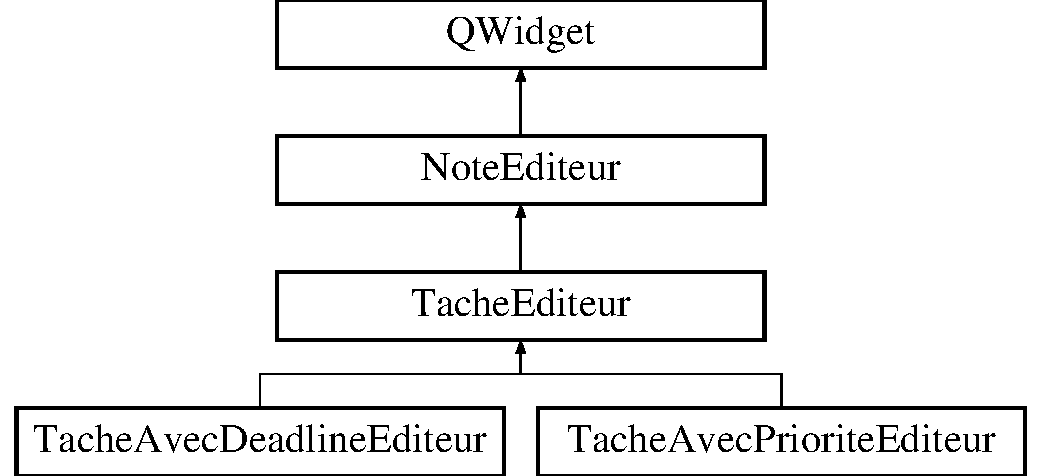
\includegraphics[height=4.000000cm]{class_tache_editeur}
\end{center}
\end{figure}
\subsection*{Connecteurs publics}
\begin{DoxyCompactItemize}
\item 
\hypertarget{class_tache_editeur_acfa771785cdea091ca5c03288c79c51a}{void \hyperlink{class_tache_editeur_acfa771785cdea091ca5c03288c79c51a}{extensionsave} ()}\label{class_tache_editeur_acfa771785cdea091ca5c03288c79c51a}

\begin{DoxyCompactList}\small\item\em Définit la sauvegarde selon la sous-\/classe de note (appelée par \hyperlink{class_note_editeur_a605b1bca885c25460cb7d8863d1f3d03}{save()}) \end{DoxyCompactList}\item 
\hypertarget{class_tache_editeur_aed4f893926b463e92086aa8553bd5d82}{void \hyperlink{class_tache_editeur_aed4f893926b463e92086aa8553bd5d82}{extensionsetasactual} ()}\label{class_tache_editeur_aed4f893926b463e92086aa8553bd5d82}

\begin{DoxyCompactList}\small\item\em Définit l'actualisation selon la sous-\/classe de la note (appelée par \hyperlink{class_note_editeur_a857f285628a0b7dcb6a69b18c977aa71}{set\-As\-Actual()}) \end{DoxyCompactList}\item 
\hypertarget{class_tache_editeur_a22a45dfa8b15b5b57076b01bf1a73640}{void \hyperlink{class_tache_editeur_a22a45dfa8b15b5b57076b01bf1a73640}{create} ()}\label{class_tache_editeur_a22a45dfa8b15b5b57076b01bf1a73640}

\begin{DoxyCompactList}\small\item\em Création d'un nouvel objet tâche depuis le \hyperlink{class_tache_editeur}{Tache\-Editeur}. \end{DoxyCompactList}\end{DoxyCompactItemize}
\subsection*{Fonctions membres publiques}
\begin{DoxyCompactItemize}
\item 
\hyperlink{class_tache_editeur_a0a8293ff8440d43d354e87445518fe7b}{Tache\-Editeur} (\hyperlink{class_tache}{Tache} \&t, Q\-Widget $\ast$parent=0)
\begin{DoxyCompactList}\small\item\em Constructeur. \end{DoxyCompactList}\item 
\hypertarget{class_tache_editeur_aaa74a2bfef09f536de419b3ac47d91e5}{\hyperlink{class_tache_editeur_aaa74a2bfef09f536de419b3ac47d91e5}{Tache\-Editeur} (Q\-Widget $\ast$parent=0)}\label{class_tache_editeur_aaa74a2bfef09f536de419b3ac47d91e5}

\begin{DoxyCompactList}\small\item\em Surcharge de constructeur si on n'a pas de tâche à afficher. \end{DoxyCompactList}\item 
\hypertarget{class_tache_editeur_ab46e82dc71f4093879dd08b9012f98c7}{Q\-Radio\-Button $\ast$ \hyperlink{class_tache_editeur_ab46e82dc71f4093879dd08b9012f98c7}{get\-Check\-\_\-attente} ()}\label{class_tache_editeur_ab46e82dc71f4093879dd08b9012f98c7}

\begin{DoxyCompactList}\small\item\em Récupère le bouton radio \char`\"{}tâche en attente\char`\"{}. \end{DoxyCompactList}\item 
\hypertarget{class_tache_editeur_a5a00a29449595fb0c38d5d8eee2500e5}{Q\-Radio\-Button $\ast$ \hyperlink{class_tache_editeur_a5a00a29449595fb0c38d5d8eee2500e5}{get\-Check\-\_\-cours} ()}\label{class_tache_editeur_a5a00a29449595fb0c38d5d8eee2500e5}

\begin{DoxyCompactList}\small\item\em Récupère le bouton radio \char`\"{}tâche en cours\char`\"{}. \end{DoxyCompactList}\item 
\hypertarget{class_tache_editeur_a898e7562d643a300fa85113baed41a5b}{Q\-Radio\-Button $\ast$ \hyperlink{class_tache_editeur_a898e7562d643a300fa85113baed41a5b}{get\-Check\-\_\-terminee} ()}\label{class_tache_editeur_a898e7562d643a300fa85113baed41a5b}

\begin{DoxyCompactList}\small\item\em Récupère le bouton radio \char`\"{}tâche terminée\char`\"{}. \end{DoxyCompactList}\item 
\hypertarget{class_tache_editeur_acfec99ee9c6b73686543e1c24a87fd65}{Q\-Text\-Edit $\ast$ \hyperlink{class_tache_editeur_acfec99ee9c6b73686543e1c24a87fd65}{get\-Text} ()}\label{class_tache_editeur_acfec99ee9c6b73686543e1c24a87fd65}

\begin{DoxyCompactList}\small\item\em Récupère le contenu de la tâche. \end{DoxyCompactList}\item 
\hypertarget{class_tache_editeur_a1e77083a97efcfb689268852d32fcdb4}{void \hyperlink{class_tache_editeur_a1e77083a97efcfb689268852d32fcdb4}{blockall} ()}\label{class_tache_editeur_a1e77083a97efcfb689268852d32fcdb4}

\begin{DoxyCompactList}\small\item\em Permet d'interdire toute action à l'utilisateur (désactive tous les boutons) \end{DoxyCompactList}\end{DoxyCompactItemize}
\subsection*{Attributs protégés}
\begin{DoxyCompactItemize}
\item 
\hypertarget{class_tache_editeur_a9e01c2cf0f6512e5c0b879b600f69664}{Q\-Label $\ast$ {\bfseries text1}}\label{class_tache_editeur_a9e01c2cf0f6512e5c0b879b600f69664}

\item 
\hypertarget{class_tache_editeur_acdd7ae1e4b7476e8713ecb7a0d02b5cb}{Q\-Text\-Edit $\ast$ {\bfseries text}}\label{class_tache_editeur_acdd7ae1e4b7476e8713ecb7a0d02b5cb}

\item 
\hypertarget{class_tache_editeur_a010ba6dd713c2c7ad5df167bf439568a}{Q\-Radio\-Button $\ast$ {\bfseries check\-\_\-attente}}\label{class_tache_editeur_a010ba6dd713c2c7ad5df167bf439568a}

\item 
\hypertarget{class_tache_editeur_a3bbbd65e667e6e0cd7ddaea05d3961a8}{Q\-Radio\-Button $\ast$ {\bfseries check\-\_\-cours}}\label{class_tache_editeur_a3bbbd65e667e6e0cd7ddaea05d3961a8}

\item 
\hypertarget{class_tache_editeur_a6b4498fa419389c0c81c8d91f31e02a0}{Q\-Radio\-Button $\ast$ {\bfseries check\-\_\-terminee}}\label{class_tache_editeur_a6b4498fa419389c0c81c8d91f31e02a0}

\end{DoxyCompactItemize}


\subsection{Description détaillée}
Permet de visualiser et modifier les tâches sans deadline ni priorité (interface). 

Classe qui est par la suite utilisée pour réaliser l'ensemble de l'interface graphiue (\hyperlink{interface_8h}{interface.\-h}). 

\subsection{Documentation des constructeurs et destructeur}
\hypertarget{class_tache_editeur_a0a8293ff8440d43d354e87445518fe7b}{\index{Tache\-Editeur@{Tache\-Editeur}!Tache\-Editeur@{Tache\-Editeur}}
\index{Tache\-Editeur@{Tache\-Editeur}!TacheEditeur@{Tache\-Editeur}}
\subsubsection[{Tache\-Editeur}]{\setlength{\rightskip}{0pt plus 5cm}Tache\-Editeur\-::\-Tache\-Editeur (
\begin{DoxyParamCaption}
\item[{{\bf Tache} \&}]{t, }
\item[{Q\-Widget $\ast$}]{parent = {\ttfamily 0}}
\end{DoxyParamCaption}
)}}\label{class_tache_editeur_a0a8293ff8440d43d354e87445518fe7b}


Constructeur. 


\begin{DoxyParams}{Paramètres}
{\em t} & Tâche à afficher \\
\hline
\end{DoxyParams}


La documentation de cette classe a été générée à partir des fichiers suivants \-:\begin{DoxyCompactItemize}
\item 
/home/camille/\-Documents/\-U\-T\-C/\-H\-U04/\-L\-O21/\-Projet/\-Projet/\hyperlink{noteediteur_8h}{noteediteur.\-h}\item 
/home/camille/\-Documents/\-U\-T\-C/\-H\-U04/\-L\-O21/\-Projet/\-Projet/noteediteur.\-cpp\end{DoxyCompactItemize}

\hypertarget{class_vue_principale}{\section{Référence de la classe Vue\-Principale}
\label{class_vue_principale}\index{Vue\-Principale@{Vue\-Principale}}
}


Représente la fenêtre principale de l'application.  




{\ttfamily \#include $<$interface.\-h$>$}

Graphe d'héritage de Vue\-Principale\-:\begin{figure}[H]
\begin{center}
\leavevmode
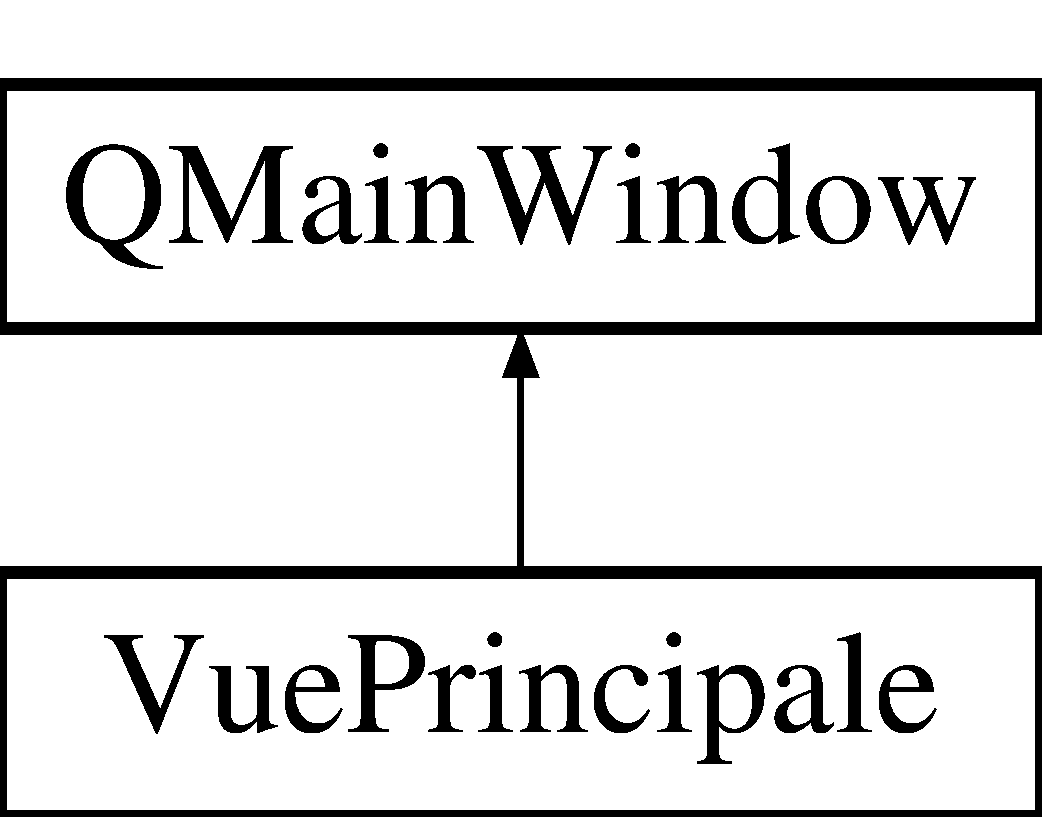
\includegraphics[height=2.000000cm]{class_vue_principale}
\end{center}
\end{figure}
\subsection*{Fonctions membres publiques}
\begin{DoxyCompactItemize}
\item 
void \hyperlink{class_vue_principale_a38a2850977156eaee637de1be6b9991a}{affichage\-\_\-central} ()
\begin{DoxyCompactList}\small\item\em Permet la création \& l'affichage de la partie centrale de la fenêtre. \end{DoxyCompactList}\item 
void \hyperlink{class_vue_principale_a2ed333250733915a381e15042df3bd35}{affichage\-\_\-droit} ()
\begin{DoxyCompactList}\small\item\em Permet la création \& l'affichage de la partie droite de la fenêtre. \end{DoxyCompactList}\item 
void \hyperlink{class_vue_principale_ab85635081670f7072008344d28b5b603}{affichage\-\_\-gauche} ()
\begin{DoxyCompactList}\small\item\em Permet la création \& l'affichage de la partie gauche de la fenêtre. \end{DoxyCompactList}\item 
void \hyperlink{class_vue_principale_ae06449e378e3a1426bd81a0d00447c8b}{creer\-Menu} ()
\begin{DoxyCompactList}\small\item\em Permet la création \& l'affichage du menu. \end{DoxyCompactList}\end{DoxyCompactItemize}
\subsection*{Fonctions membres publiques statiques}
\begin{DoxyCompactItemize}
\item 
static \hyperlink{class_vue_principale}{Vue\-Principale} \& \hyperlink{class_vue_principale_ac475702859be52ac07b329663c24a56b}{get\-Instance} (\hyperlink{class_note}{Note} $\ast$n=0)
\begin{DoxyCompactList}\small\item\em Permet d'accéder au seul objet de la classe \hyperlink{class_vue_principale}{Vue\-Principale} (D\-P Singleton). \end{DoxyCompactList}\end{DoxyCompactItemize}
\subsection*{Fonctions membres protégées}
\begin{DoxyCompactItemize}
\item 
void \hyperlink{class_vue_principale_aac7af04920ca134b4fdf10f0e2693724}{close\-Event} (Q\-Close\-Event $\ast$event)
\begin{DoxyCompactList}\small\item\em Permet de gérer le vidage automatique de la corbeille. \end{DoxyCompactList}\end{DoxyCompactItemize}
\subsection*{Connecteurs privés}
\begin{DoxyCompactItemize}
\item 
\hypertarget{class_vue_principale_a242a1a9732b6c7997fa5998c25678a81}{void \hyperlink{class_vue_principale_a242a1a9732b6c7997fa5998c25678a81}{show\-Relations} ()}\label{class_vue_principale_a242a1a9732b6c7997fa5998c25678a81}

\begin{DoxyCompactList}\small\item\em Appelle le constructeur de la fenêtre secondaire (gestion \& visualisation des relations) \end{DoxyCompactList}\item 
\hypertarget{class_vue_principale_a726c780ade730bd88e15cfc6e63bb6a4}{void \hyperlink{class_vue_principale_a726c780ade730bd88e15cfc6e63bb6a4}{afficage\-Arbo} ()}\label{class_vue_principale_a726c780ade730bd88e15cfc6e63bb6a4}

\begin{DoxyCompactList}\small\item\em gère la partie droite (masque ou affiche l'arborescence) \end{DoxyCompactList}\item 
void \hyperlink{class_vue_principale_a487dbd07f0f5f81327606cc8c5235cef}{afficher\-\_\-note} (Q\-Tree\-Widget\-Item $\ast$item)
\begin{DoxyCompactList}\small\item\em Permet l'affichage d'une nouvelle note. \end{DoxyCompactList}\item 
void \hyperlink{class_vue_principale_ad72391d3e8bc1f37cd664657570c6518}{afficher\-\_\-version} (Q\-Tree\-Widget\-Item $\ast$item)
\begin{DoxyCompactList}\small\item\em Permet l'affichage d'une autre version de la note. \end{DoxyCompactList}\item 
void \hyperlink{class_vue_principale_a61cad396c2c3ed664bb8b45cfdd2e188}{new\-\_\-note} (int i)
\begin{DoxyCompactList}\small\item\em Permet la création d'une nouvelle note. \end{DoxyCompactList}\item 
\hypertarget{class_vue_principale_a205e5f51dbbe6d0d648ec52e629d2e6c}{void \hyperlink{class_vue_principale_a205e5f51dbbe6d0d648ec52e629d2e6c}{actualiser\-\_\-fenetre} ()}\label{class_vue_principale_a205e5f51dbbe6d0d648ec52e629d2e6c}

\begin{DoxyCompactList}\small\item\em Permet d'actualiser l'affichage si une note/relation a été modifiée/créée/supprimée. \end{DoxyCompactList}\item 
\hypertarget{class_vue_principale_a2f77ec0647f3ac52ffedc0ad668f1646}{void \hyperlink{class_vue_principale_a2f77ec0647f3ac52ffedc0ad668f1646}{creer\-Article} ()}\label{class_vue_principale_a2f77ec0647f3ac52ffedc0ad668f1646}

\begin{DoxyCompactList}\small\item\em Permet de créer un nouvel article via la barre de menu. \end{DoxyCompactList}\item 
\hypertarget{class_vue_principale_a61157e05ff0f5e01ba286ab5cd374fd2}{void \hyperlink{class_vue_principale_a61157e05ff0f5e01ba286ab5cd374fd2}{creer\-Tache} ()}\label{class_vue_principale_a61157e05ff0f5e01ba286ab5cd374fd2}

\begin{DoxyCompactList}\small\item\em Permet de créer une nouvelle tâche sans deadline/priorité via la barre de menu. \end{DoxyCompactList}\item 
\hypertarget{class_vue_principale_a97ebca7d1567e54e1105b8fea1c1ca51}{void \hyperlink{class_vue_principale_a97ebca7d1567e54e1105b8fea1c1ca51}{creer\-Tache\-Deadline} ()}\label{class_vue_principale_a97ebca7d1567e54e1105b8fea1c1ca51}

\begin{DoxyCompactList}\small\item\em Permet de créer une nouvelle tâche avec deadline via la barre de menu. \end{DoxyCompactList}\item 
\hypertarget{class_vue_principale_aee6a12d4a49be4d8282421ad4de5d50f}{void \hyperlink{class_vue_principale_aee6a12d4a49be4d8282421ad4de5d50f}{creer\-Fichier} ()}\label{class_vue_principale_aee6a12d4a49be4d8282421ad4de5d50f}

\begin{DoxyCompactList}\small\item\em Permet de créer un nouveau fichier via la barre de menu. \end{DoxyCompactList}\item 
\hypertarget{class_vue_principale_a7d75be5c40167a67b69a91944210e299}{void \hyperlink{class_vue_principale_a7d75be5c40167a67b69a91944210e299}{creer\-Tache\-Priorite} ()}\label{class_vue_principale_a7d75be5c40167a67b69a91944210e299}

\begin{DoxyCompactList}\small\item\em Permet de créer une nouvelle tâche avec priorité via la barre de menu. \end{DoxyCompactList}\end{DoxyCompactItemize}
\subsection*{Fonctions membres privées}
\begin{DoxyCompactItemize}
\item 
\hyperlink{class_vue_principale_aa956c73fa9b92d2031058a42923b58cb}{Vue\-Principale} (\hyperlink{class_note}{Note} $\ast$n=0)
\begin{DoxyCompactList}\small\item\em Constructeur de la fenêtre. \end{DoxyCompactList}\end{DoxyCompactItemize}
\subsection*{Attributs privés}
\begin{DoxyCompactItemize}
\item 
\hypertarget{class_vue_principale_a19079699098c0c8846f360f81caa9562}{unsigned int {\bfseries marqueur}}\label{class_vue_principale_a19079699098c0c8846f360f81caa9562}

\item 
\hypertarget{class_vue_principale_a77071012fcd0ab3c5b917cf9cf3932b6}{Q\-Widget $\ast$ {\bfseries zone\-Centrale}}\label{class_vue_principale_a77071012fcd0ab3c5b917cf9cf3932b6}

\item 
\hypertarget{class_vue_principale_a733fa80891be7be01dd2a494338011c2}{Q\-H\-Box\-Layout $\ast$ {\bfseries layout\-Principal}}\label{class_vue_principale_a733fa80891be7be01dd2a494338011c2}

\item 
\hypertarget{class_vue_principale_aa10cc91367ac162477a61d61bc3983d6}{Q\-Push\-Button $\ast$ {\bfseries actualiser}}\label{class_vue_principale_aa10cc91367ac162477a61d61bc3983d6}

\item 
\hypertarget{class_vue_principale_a21ca0b616e1b8573996bacd0788a4d5f}{Q\-Push\-Button $\ast$ {\bfseries arborescence}}\label{class_vue_principale_a21ca0b616e1b8573996bacd0788a4d5f}

\item 
\hypertarget{class_vue_principale_aa5c8a23312070df19df91b4a11a0f0f9}{Q\-Action $\ast$ {\bfseries action\-Supp}}\label{class_vue_principale_aa5c8a23312070df19df91b4a11a0f0f9}

\item 
\hypertarget{class_vue_principale_ad488b8bbb081be458ea8e6bc91855643}{Q\-Menu $\ast$ {\bfseries menu\-Fichier}}\label{class_vue_principale_ad488b8bbb081be458ea8e6bc91855643}

\item 
\hypertarget{class_vue_principale_a71889c8911ea8e048f7929ee018762da}{Q\-Group\-Box $\ast$ {\bfseries gauche}}\label{class_vue_principale_a71889c8911ea8e048f7929ee018762da}

\item 
\hypertarget{class_vue_principale_a4e6033054ca0180b87c473ac62355614}{Q\-Group\-Box $\ast$ {\bfseries centre}}\label{class_vue_principale_a4e6033054ca0180b87c473ac62355614}

\item 
\hypertarget{class_vue_principale_ae504dae6ea9c3c76f1bb7d3497b60b1f}{\hyperlink{class_note}{Note} $\ast$ {\bfseries note}}\label{class_vue_principale_ae504dae6ea9c3c76f1bb7d3497b60b1f}

\item 
\hypertarget{class_vue_principale_ac887b69330a47fc775a85a45fca3247e}{\hyperlink{class_note_editeur}{Note\-Editeur} $\ast$ {\bfseries note\-Edit}}\label{class_vue_principale_ac887b69330a47fc775a85a45fca3247e}

\item 
\hypertarget{class_vue_principale_a786106f1c4637d79748040b21e81876e}{Q\-Action $\ast$ {\bfseries action\-Save}}\label{class_vue_principale_a786106f1c4637d79748040b21e81876e}

\item 
\hypertarget{class_vue_principale_ae1ec36e06063e6097ce4e4c956142c6e}{bool {\bfseries save\-Active}}\label{class_vue_principale_ae1ec36e06063e6097ce4e4c956142c6e}

\item 
\hypertarget{class_vue_principale_a89b04596c58cd9ff7fa1a8526ed29289}{Q\-Group\-Box $\ast$ {\bfseries droite}}\label{class_vue_principale_a89b04596c58cd9ff7fa1a8526ed29289}

\item 
\hypertarget{class_vue_principale_aa0248272de083bb9cd0cb6a496daceb4}{bool {\bfseries arbo\-Visible}}\label{class_vue_principale_aa0248272de083bb9cd0cb6a496daceb4}

\item 
\hypertarget{class_vue_principale_a7c6eb51ba5b96ac5dca69fc3ffd65784}{Q\-Push\-Button $\ast$ {\bfseries relation\-\_\-details}}\label{class_vue_principale_a7c6eb51ba5b96ac5dca69fc3ffd65784}

\end{DoxyCompactItemize}
\subsection*{Attributs privés statiques}
\begin{DoxyCompactItemize}
\item 
\hypertarget{class_vue_principale_ac6d04800f0fbda43d2ec1127815c07de}{static \hyperlink{class_vue_principale}{Vue\-Principale} $\ast$ {\bfseries instance}}\label{class_vue_principale_ac6d04800f0fbda43d2ec1127815c07de}

\end{DoxyCompactItemize}


\subsection{Description détaillée}
Représente la fenêtre principale de l'application. 

Permet la visualisation/modification d'une note \& de l'arborescence de ses relations, la visualisation des notes actives, des tâches et des notes archivées. Permet aussi la création d'une nouvelle note. 

\subsection{Documentation des constructeurs et destructeur}
\hypertarget{class_vue_principale_aa956c73fa9b92d2031058a42923b58cb}{\index{Vue\-Principale@{Vue\-Principale}!Vue\-Principale@{Vue\-Principale}}
\index{Vue\-Principale@{Vue\-Principale}!VuePrincipale@{Vue\-Principale}}
\subsubsection[{Vue\-Principale}]{\setlength{\rightskip}{0pt plus 5cm}Vue\-Principale\-::\-Vue\-Principale (
\begin{DoxyParamCaption}
\item[{{\bf Note} $\ast$}]{n = {\ttfamily 0}}
\end{DoxyParamCaption}
)\hspace{0.3cm}{\ttfamily [private]}}}\label{class_vue_principale_aa956c73fa9b92d2031058a42923b58cb}


Constructeur de la fenêtre. 

En privé pour le D\-P singleton. 
\begin{DoxyParams}{Paramètres}
{\em n} & \hyperlink{class_note}{Note} à afficher (par défaut, on n'affiche aucune note). \\
\hline
\end{DoxyParams}


\subsection{Documentation des fonctions membres}
\hypertarget{class_vue_principale_a38a2850977156eaee637de1be6b9991a}{\index{Vue\-Principale@{Vue\-Principale}!affichage\-\_\-central@{affichage\-\_\-central}}
\index{affichage\-\_\-central@{affichage\-\_\-central}!VuePrincipale@{Vue\-Principale}}
\subsubsection[{affichage\-\_\-central}]{\setlength{\rightskip}{0pt plus 5cm}void Vue\-Principale\-::affichage\-\_\-central (
\begin{DoxyParamCaption}
{}
\end{DoxyParamCaption}
)}}\label{class_vue_principale_a38a2850977156eaee637de1be6b9991a}


Permet la création \& l'affichage de la partie centrale de la fenêtre. 

Utilisée dans le constructeur. \hypertarget{class_vue_principale_a2ed333250733915a381e15042df3bd35}{\index{Vue\-Principale@{Vue\-Principale}!affichage\-\_\-droit@{affichage\-\_\-droit}}
\index{affichage\-\_\-droit@{affichage\-\_\-droit}!VuePrincipale@{Vue\-Principale}}
\subsubsection[{affichage\-\_\-droit}]{\setlength{\rightskip}{0pt plus 5cm}void Vue\-Principale\-::affichage\-\_\-droit (
\begin{DoxyParamCaption}
{}
\end{DoxyParamCaption}
)}}\label{class_vue_principale_a2ed333250733915a381e15042df3bd35}


Permet la création \& l'affichage de la partie droite de la fenêtre. 

Utilisée dans le constructeur. \hypertarget{class_vue_principale_ab85635081670f7072008344d28b5b603}{\index{Vue\-Principale@{Vue\-Principale}!affichage\-\_\-gauche@{affichage\-\_\-gauche}}
\index{affichage\-\_\-gauche@{affichage\-\_\-gauche}!VuePrincipale@{Vue\-Principale}}
\subsubsection[{affichage\-\_\-gauche}]{\setlength{\rightskip}{0pt plus 5cm}void Vue\-Principale\-::affichage\-\_\-gauche (
\begin{DoxyParamCaption}
{}
\end{DoxyParamCaption}
)}}\label{class_vue_principale_ab85635081670f7072008344d28b5b603}


Permet la création \& l'affichage de la partie gauche de la fenêtre. 

Utilisée dans le constructeur. \hypertarget{class_vue_principale_a487dbd07f0f5f81327606cc8c5235cef}{\index{Vue\-Principale@{Vue\-Principale}!afficher\-\_\-note@{afficher\-\_\-note}}
\index{afficher\-\_\-note@{afficher\-\_\-note}!VuePrincipale@{Vue\-Principale}}
\subsubsection[{afficher\-\_\-note}]{\setlength{\rightskip}{0pt plus 5cm}void Vue\-Principale\-::afficher\-\_\-note (
\begin{DoxyParamCaption}
\item[{Q\-Tree\-Widget\-Item $\ast$}]{item}
\end{DoxyParamCaption}
)\hspace{0.3cm}{\ttfamily [private]}, {\ttfamily [slot]}}}\label{class_vue_principale_a487dbd07f0f5f81327606cc8c5235cef}


Permet l'affichage d'une nouvelle note. 

Slot appelé lorsque l'utilisateur sélectionne une note dans l'arborescence ou dans la colonne de gauche \hypertarget{class_vue_principale_ad72391d3e8bc1f37cd664657570c6518}{\index{Vue\-Principale@{Vue\-Principale}!afficher\-\_\-version@{afficher\-\_\-version}}
\index{afficher\-\_\-version@{afficher\-\_\-version}!VuePrincipale@{Vue\-Principale}}
\subsubsection[{afficher\-\_\-version}]{\setlength{\rightskip}{0pt plus 5cm}void Vue\-Principale\-::afficher\-\_\-version (
\begin{DoxyParamCaption}
\item[{Q\-Tree\-Widget\-Item $\ast$}]{item}
\end{DoxyParamCaption}
)\hspace{0.3cm}{\ttfamily [private]}, {\ttfamily [slot]}}}\label{class_vue_principale_ad72391d3e8bc1f37cd664657570c6518}


Permet l'affichage d'une autre version de la note. 

Slot appelé lorsque l'utilisateur sélectionne une autre version de la note visualisée (colonne de droite). \hypertarget{class_vue_principale_aac7af04920ca134b4fdf10f0e2693724}{\index{Vue\-Principale@{Vue\-Principale}!close\-Event@{close\-Event}}
\index{close\-Event@{close\-Event}!VuePrincipale@{Vue\-Principale}}
\subsubsection[{close\-Event}]{\setlength{\rightskip}{0pt plus 5cm}void Vue\-Principale\-::close\-Event (
\begin{DoxyParamCaption}
\item[{Q\-Close\-Event $\ast$}]{event}
\end{DoxyParamCaption}
)\hspace{0.3cm}{\ttfamily [protected]}}}\label{class_vue_principale_aac7af04920ca134b4fdf10f0e2693724}


Permet de gérer le vidage automatique de la corbeille. 

Si l'option de vidage automatique est activée dans le menu, on ferme la fenetre et on vide la corbeille. Sinon, on affiche une boîte de dialogue demandant à l'utilisateur s'il désire supprimer le contenu de la corbeille au moment de la fermeture de l'application. 
\begin{DoxyParams}{Paramètres}
{\em event} & Si l'option de vidage automatique est activée ou non. \\
\hline
\end{DoxyParams}
\hypertarget{class_vue_principale_ae06449e378e3a1426bd81a0d00447c8b}{\index{Vue\-Principale@{Vue\-Principale}!creer\-Menu@{creer\-Menu}}
\index{creer\-Menu@{creer\-Menu}!VuePrincipale@{Vue\-Principale}}
\subsubsection[{creer\-Menu}]{\setlength{\rightskip}{0pt plus 5cm}void Vue\-Principale\-::creer\-Menu (
\begin{DoxyParamCaption}
{}
\end{DoxyParamCaption}
)}}\label{class_vue_principale_ae06449e378e3a1426bd81a0d00447c8b}


Permet la création \& l'affichage du menu. 

Utilisée dans le constructeur. \hypertarget{class_vue_principale_ac475702859be52ac07b329663c24a56b}{\index{Vue\-Principale@{Vue\-Principale}!get\-Instance@{get\-Instance}}
\index{get\-Instance@{get\-Instance}!VuePrincipale@{Vue\-Principale}}
\subsubsection[{get\-Instance}]{\setlength{\rightskip}{0pt plus 5cm}{\bf Vue\-Principale} \& Vue\-Principale\-::get\-Instance (
\begin{DoxyParamCaption}
\item[{{\bf Note} $\ast$}]{n = {\ttfamily 0}}
\end{DoxyParamCaption}
)\hspace{0.3cm}{\ttfamily [static]}}}\label{class_vue_principale_ac475702859be52ac07b329663c24a56b}


Permet d'accéder au seul objet de la classe \hyperlink{class_vue_principale}{Vue\-Principale} (D\-P Singleton). 

Crée une instance s'il n'en existe pas, retourne l'instance déjà existante sinon. 
\begin{DoxyParams}{Paramètres}
{\em n} & La note que l'on souhaite afficher (par défaut, on n'affiche aucune note). \\
\hline
\end{DoxyParams}
\begin{DoxyReturn}{Renvoie}
Une référence sur la seule instance de la fenêtre. 
\end{DoxyReturn}
\hypertarget{class_vue_principale_a61cad396c2c3ed664bb8b45cfdd2e188}{\index{Vue\-Principale@{Vue\-Principale}!new\-\_\-note@{new\-\_\-note}}
\index{new\-\_\-note@{new\-\_\-note}!VuePrincipale@{Vue\-Principale}}
\subsubsection[{new\-\_\-note}]{\setlength{\rightskip}{0pt plus 5cm}void Vue\-Principale\-::new\-\_\-note (
\begin{DoxyParamCaption}
\item[{int}]{i}
\end{DoxyParamCaption}
)\hspace{0.3cm}{\ttfamily [private]}, {\ttfamily [slot]}}}\label{class_vue_principale_a61cad396c2c3ed664bb8b45cfdd2e188}


Permet la création d'une nouvelle note. 


\begin{DoxyParams}{Paramètres}
{\em i} & Marqueur, indique le type de note à créer (1 pour \hyperlink{class_article}{Article}, 2 pour \hyperlink{class_tache}{Tache}, 3 pour \hyperlink{class_tache_avec_priorite}{Tache\-Avec\-Priorite}, 4 pour \hyperlink{class_tache_avec_deadline}{Tache\-Avec\-Deadline}, 5 pour \hyperlink{class_fichier}{Fichier}) \\
\hline
\end{DoxyParams}


La documentation de cette classe a été générée à partir des fichiers suivants \-:\begin{DoxyCompactItemize}
\item 
/home/camille/\-Documents/\-U\-T\-C/\-H\-U04/\-L\-O21/\-Projet/\-Projet/\hyperlink{interface_8h}{interface.\-h}\item 
/home/camille/\-Documents/\-U\-T\-C/\-H\-U04/\-L\-O21/\-Projet/\-Projet/\hyperlink{interface_8cpp}{interface.\-cpp}\end{DoxyCompactItemize}

\hypertarget{class_vue_secondaire}{\section{Référence de la classe Vue\-Secondaire}
\label{class_vue_secondaire}\index{Vue\-Secondaire@{Vue\-Secondaire}}
}


Représente la fenêtre secondaire de l'application (gestion des relations).  




{\ttfamily \#include $<$interface.\-h$>$}

Graphe d'héritage de Vue\-Secondaire\-:\begin{figure}[H]
\begin{center}
\leavevmode
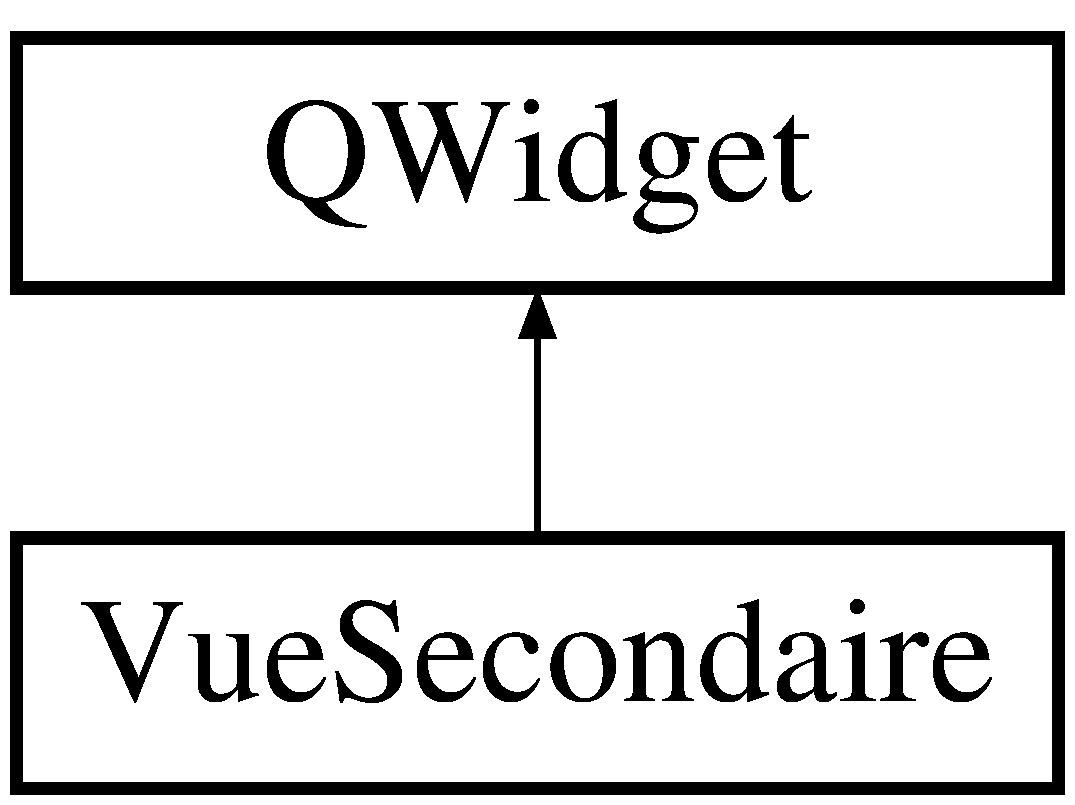
\includegraphics[height=2.000000cm]{class_vue_secondaire}
\end{center}
\end{figure}
\subsection*{Fonctions membres publiques}
\begin{DoxyCompactItemize}
\item 
void \hyperlink{class_vue_secondaire_a79707eb0d8aaddb12d1e1da5b89da844}{affichage\-\_\-central} ()
\begin{DoxyCompactList}\small\item\em Permet la création \& l'affichage de la partie centrale de la fenêtre. \end{DoxyCompactList}\item 
void \hyperlink{class_vue_secondaire_a8af89508ca4dfc46c7474e7fed627400}{affichage\-\_\-gauche} ()
\begin{DoxyCompactList}\small\item\em Permet la création \& l'affichage de la partie gauche de la fenêtre. \end{DoxyCompactList}\end{DoxyCompactItemize}
\subsection*{Fonctions membres publiques statiques}
\begin{DoxyCompactItemize}
\item 
static \hyperlink{class_vue_secondaire}{Vue\-Secondaire} \& \hyperlink{class_vue_secondaire_a455f8674109c95488ca12c8ee6b5861e}{get\-Instance} ()
\begin{DoxyCompactList}\small\item\em Permet d'accéder au seul objet de la classe \hyperlink{class_vue_secondaire}{Vue\-Secondaire} (D\-P Singleton). \end{DoxyCompactList}\end{DoxyCompactItemize}
\subsection*{Connecteurs privés}
\begin{DoxyCompactItemize}
\item 
void \hyperlink{class_vue_secondaire_af939340a1323aa49d52333b7f49d8e64}{open\-Relation} (Q\-Tree\-Widget\-Item $\ast$item)
\begin{DoxyCompactList}\small\item\em Ouvre le relation\-Editeur d'une relation sélectionnée par l'utilisateur. \end{DoxyCompactList}\item 
\hypertarget{class_vue_secondaire_a18dd8554d253c1c2c17a03c416c45d92}{void \hyperlink{class_vue_secondaire_a18dd8554d253c1c2c17a03c416c45d92}{actualiser\-\_\-fenetre} ()}\label{class_vue_secondaire_a18dd8554d253c1c2c17a03c416c45d92}

\begin{DoxyCompactList}\small\item\em Permet d'actualiser l'affichage si une relation a été modifiée/créée/supprimée. \end{DoxyCompactList}\end{DoxyCompactItemize}
\subsection*{Attributs privés}
\begin{DoxyCompactItemize}
\item 
\hypertarget{class_vue_secondaire_ae67763136ea85968932d26f3c2363e23}{Q\-H\-Box\-Layout $\ast$ {\bfseries layout\-Principal}}\label{class_vue_secondaire_ae67763136ea85968932d26f3c2363e23}

\item 
\hypertarget{class_vue_secondaire_a2e69be7e1a13dc9918e7611ba2ef9394}{Q\-V\-Box\-Layout $\ast$ {\bfseries principal}}\label{class_vue_secondaire_a2e69be7e1a13dc9918e7611ba2ef9394}

\item 
\hypertarget{class_vue_secondaire_a0f151bf36e1bb0c9915eb90b82fb00d5}{Q\-Group\-Box $\ast$ {\bfseries centre}}\label{class_vue_secondaire_a0f151bf36e1bb0c9915eb90b82fb00d5}

\item 
\hypertarget{class_vue_secondaire_a3bcb066271a0b3183f9c34736fbe0f0c}{\hyperlink{class_relation}{Relation} $\ast$ {\bfseries relation}}\label{class_vue_secondaire_a3bcb066271a0b3183f9c34736fbe0f0c}

\item 
\hypertarget{class_vue_secondaire_a789d5ea9121cda385d58070fa34e4dc8}{\hyperlink{class_relation_editeur}{Relation\-Editeur} $\ast$ {\bfseries relation\-Edit}}\label{class_vue_secondaire_a789d5ea9121cda385d58070fa34e4dc8}

\item 
\hypertarget{class_vue_secondaire_af97140ff4a8a511ddb0e7e285666618d}{Q\-Group\-Box $\ast$ {\bfseries gauche}}\label{class_vue_secondaire_af97140ff4a8a511ddb0e7e285666618d}

\item 
\hypertarget{class_vue_secondaire_a79901bbe5834dee7a8014f10eb70d6c7}{Q\-Push\-Button $\ast$ {\bfseries quitter}}\label{class_vue_secondaire_a79901bbe5834dee7a8014f10eb70d6c7}

\item 
\hypertarget{class_vue_secondaire_a6a5663f223ae025eae5bef144e26ad0b}{Q\-Push\-Button $\ast$ {\bfseries actualiser}}\label{class_vue_secondaire_a6a5663f223ae025eae5bef144e26ad0b}

\end{DoxyCompactItemize}
\subsection*{Attributs privés statiques}
\begin{DoxyCompactItemize}
\item 
\hypertarget{class_vue_secondaire_a5cbd56d7df3b44772b5196f76788b215}{static \hyperlink{class_vue_secondaire}{Vue\-Secondaire} $\ast$ {\bfseries instance}}\label{class_vue_secondaire_a5cbd56d7df3b44772b5196f76788b215}

\end{DoxyCompactItemize}


\subsection{Description détaillée}
Représente la fenêtre secondaire de l'application (gestion des relations). 

Permet la visualisation/modification de l'ensemble des relations. La partie droite affiche les relations existantes, la partie principale permet la visualisation \& modification d'une relation en particulier. 

\subsection{Documentation des fonctions membres}
\hypertarget{class_vue_secondaire_a79707eb0d8aaddb12d1e1da5b89da844}{\index{Vue\-Secondaire@{Vue\-Secondaire}!affichage\-\_\-central@{affichage\-\_\-central}}
\index{affichage\-\_\-central@{affichage\-\_\-central}!VueSecondaire@{Vue\-Secondaire}}
\subsubsection[{affichage\-\_\-central}]{\setlength{\rightskip}{0pt plus 5cm}void Vue\-Secondaire\-::affichage\-\_\-central (
\begin{DoxyParamCaption}
{}
\end{DoxyParamCaption}
)}}\label{class_vue_secondaire_a79707eb0d8aaddb12d1e1da5b89da844}


Permet la création \& l'affichage de la partie centrale de la fenêtre. 

Utilisée dans le constructeur. \hypertarget{class_vue_secondaire_a8af89508ca4dfc46c7474e7fed627400}{\index{Vue\-Secondaire@{Vue\-Secondaire}!affichage\-\_\-gauche@{affichage\-\_\-gauche}}
\index{affichage\-\_\-gauche@{affichage\-\_\-gauche}!VueSecondaire@{Vue\-Secondaire}}
\subsubsection[{affichage\-\_\-gauche}]{\setlength{\rightskip}{0pt plus 5cm}void Vue\-Secondaire\-::affichage\-\_\-gauche (
\begin{DoxyParamCaption}
{}
\end{DoxyParamCaption}
)}}\label{class_vue_secondaire_a8af89508ca4dfc46c7474e7fed627400}


Permet la création \& l'affichage de la partie gauche de la fenêtre. 

Utilisée dans le constructeur. \hypertarget{class_vue_secondaire_a455f8674109c95488ca12c8ee6b5861e}{\index{Vue\-Secondaire@{Vue\-Secondaire}!get\-Instance@{get\-Instance}}
\index{get\-Instance@{get\-Instance}!VueSecondaire@{Vue\-Secondaire}}
\subsubsection[{get\-Instance}]{\setlength{\rightskip}{0pt plus 5cm}{\bf Vue\-Secondaire} \& Vue\-Secondaire\-::get\-Instance (
\begin{DoxyParamCaption}
{}
\end{DoxyParamCaption}
)\hspace{0.3cm}{\ttfamily [static]}}}\label{class_vue_secondaire_a455f8674109c95488ca12c8ee6b5861e}


Permet d'accéder au seul objet de la classe \hyperlink{class_vue_secondaire}{Vue\-Secondaire} (D\-P Singleton). 

Crée une instance s'il n'en existe pas, retourne l'instance déjà existante sinon. \begin{DoxyReturn}{Renvoie}
Une référence sur la seule instance de la fenêtre. 
\end{DoxyReturn}
\hypertarget{class_vue_secondaire_af939340a1323aa49d52333b7f49d8e64}{\index{Vue\-Secondaire@{Vue\-Secondaire}!open\-Relation@{open\-Relation}}
\index{open\-Relation@{open\-Relation}!VueSecondaire@{Vue\-Secondaire}}
\subsubsection[{open\-Relation}]{\setlength{\rightskip}{0pt plus 5cm}void Vue\-Secondaire\-::open\-Relation (
\begin{DoxyParamCaption}
\item[{Q\-Tree\-Widget\-Item $\ast$}]{item}
\end{DoxyParamCaption}
)\hspace{0.3cm}{\ttfamily [private]}, {\ttfamily [slot]}}}\label{class_vue_secondaire_af939340a1323aa49d52333b7f49d8e64}


Ouvre le relation\-Editeur d'une relation sélectionnée par l'utilisateur. 


\begin{DoxyParams}{Paramètres}
{\em item} & Une relation présente dans l'arborescence. \\
\hline
\end{DoxyParams}


La documentation de cette classe a été générée à partir des fichiers suivants \-:\begin{DoxyCompactItemize}
\item 
/home/camille/\-Documents/\-U\-T\-C/\-H\-U04/\-L\-O21/\-Projet/\-Projet/\hyperlink{interface_8h}{interface.\-h}\item 
/home/camille/\-Documents/\-U\-T\-C/\-H\-U04/\-L\-O21/\-Projet/\-Projet/\hyperlink{interface_8cpp}{interface.\-cpp}\end{DoxyCompactItemize}

\chapter{Documentation des fichiers}
\hypertarget{interface_8cpp}{\section{Référence du fichier /home/camille/\-Documents/\-U\-T\-C/\-H\-U04/\-L\-O21/\-Projet/\-Projet/interface.cpp}
\label{interface_8cpp}\index{/home/camille/\-Documents/\-U\-T\-C/\-H\-U04/\-L\-O21/\-Projet/\-Projet/interface.\-cpp@{/home/camille/\-Documents/\-U\-T\-C/\-H\-U04/\-L\-O21/\-Projet/\-Projet/interface.\-cpp}}
}


Définit les méthodes relatives à l'interface de l'application.  


{\ttfamily \#include $<$interface.\-h$>$}\\*
{\ttfamily \#include $<$typeinfo$>$}\\*
{\ttfamily \#include $<$Q\-Group\-Box$>$}\\*
{\ttfamily \#include $<$Q\-Form\-Layout$>$}\\*


\subsection{Description détaillée}
Définit les méthodes relatives à l'interface de l'application. Définit les méthodes relatives au \hyperlink{class_relation_editeur}{Relation\-Editeur}.

Définition des constructeurs des fenêtres principale \& secondaire ainsi que toutes les méthodes qui y sont nécessaires, et l'ensemble des slots nécessaires au fonctionnement de l'application.
\hypertarget{interface_8h}{\section{Référence du fichier /home/camille/\-Documents/\-U\-T\-C/\-H\-U04/\-L\-O21/\-Projet/\-Projet/interface.h}
\label{interface_8h}\index{/home/camille/\-Documents/\-U\-T\-C/\-H\-U04/\-L\-O21/\-Projet/\-Projet/interface.\-h@{/home/camille/\-Documents/\-U\-T\-C/\-H\-U04/\-L\-O21/\-Projet/\-Projet/interface.\-h}}
}


Définit les classes nécessaires à l'interface de l'application (fenêtres).  


{\ttfamily \#include $<$Q\-Application$>$}\\*
{\ttfamily \#include $<$Q\-File\-Dialog$>$}\\*
{\ttfamily \#include $<$Q\-Widget$>$}\\*
{\ttfamily \#include $<$Q\-Label$>$}\\*
{\ttfamily \#include $<$Q\-Line\-Edit$>$}\\*
{\ttfamily \#include $<$Q\-Text\-Edit$>$}\\*
{\ttfamily \#include $<$Q\-Push\-Button$>$}\\*
{\ttfamily \#include $<$Q\-V\-Box\-Layout$>$}\\*
{\ttfamily \#include $<$Q\-Date$>$}\\*
{\ttfamily \#include $<$Q\-Date\-Edit$>$}\\*
{\ttfamily \#include $<$Q\-Message\-Box$>$}\\*
{\ttfamily \#include $<$Qt\-Gui$>$}\\*
{\ttfamily \#include $<$Q\-Group\-Box$>$}\\*
{\ttfamily \#include $<$Q\-Dock\-Widget$>$}\\*
{\ttfamily \#include $<$Q\-Main\-Window$>$}\\*
{\ttfamily \#include $<$Q\-Menu\-Bar$>$}\\*
{\ttfamily \#include $<$Q\-Menu$>$}\\*
{\ttfamily \#include $<$Q\-Shortcut$>$}\\*
{\ttfamily \#include $<$Q\-Key\-Sequence$>$}\\*
{\ttfamily \#include $<$Q\-Tree\-Widget$>$}\\*
{\ttfamily \#include $<$Q\-Tree\-Widget\-Item$>$}\\*
{\ttfamily \#include $<$Q\-Form\-Layout$>$}\\*
{\ttfamily \#include $<$note.\-h$>$}\\*
{\ttfamily \#include $<$noteediteur.\-h$>$}\\*
{\ttfamily \#include $<$relation.\-h$>$}\\*
{\ttfamily \#include $<$relationediteur.\-h$>$}\\*
\subsection*{Classes}
\begin{DoxyCompactItemize}
\item 
class \hyperlink{class_interface_exception}{Interface\-Exception}
\begin{DoxyCompactList}\small\item\em Permet de gérer les exceptions liées à l'interface. \end{DoxyCompactList}\item 
class \hyperlink{class_vue_principale}{Vue\-Principale}
\begin{DoxyCompactList}\small\item\em Représente la fenêtre principale de l'application. \end{DoxyCompactList}\item 
class \hyperlink{class_vue_secondaire}{Vue\-Secondaire}
\begin{DoxyCompactList}\small\item\em Représente la fenêtre secondaire de l'application (gestion des relations). \end{DoxyCompactList}\end{DoxyCompactItemize}


\subsection{Description détaillée}
Définit les classes nécessaires à l'interface de l'application (fenêtres). 
\hypertarget{note_8cpp}{\section{Référence du fichier /home/camille/\-Documents/\-U\-T\-C/\-H\-U04/\-L\-O21/\-Projet/\-Projet/note.cpp}
\label{note_8cpp}\index{/home/camille/\-Documents/\-U\-T\-C/\-H\-U04/\-L\-O21/\-Projet/\-Projet/note.\-cpp@{/home/camille/\-Documents/\-U\-T\-C/\-H\-U04/\-L\-O21/\-Projet/\-Projet/note.\-cpp}}
}


Définit les méthodes relatives aux classes note, ses dérivées et \hyperlink{class_notes_manager}{Notes\-Manager}.  


{\ttfamily \#include \char`\"{}note.\-h\char`\"{}}\\*
{\ttfamily \#include \char`\"{}relation.\-h\char`\"{}}\\*
{\ttfamily \#include $<$Q\-File$>$}\\*
{\ttfamily \#include $<$Q\-Text\-Codec$>$}\\*
{\ttfamily \#include $<$Qt\-Xml$>$}\\*
{\ttfamily \#include $<$Q\-Message\-Box$>$}\\*
{\ttfamily \#include $<$typeinfo$>$}\\*
{\ttfamily \#include $<$Q\-Debug$>$}\\*


\subsection{Description détaillée}
Définit les méthodes relatives aux classes note, ses dérivées et \hyperlink{class_notes_manager}{Notes\-Manager}. 
\hypertarget{note_8h}{\section{Référence du fichier /home/camille/\-Documents/\-U\-T\-C/\-H\-U04/\-L\-O21/\-Projet/\-Projet/note.h}
\label{note_8h}\index{/home/camille/\-Documents/\-U\-T\-C/\-H\-U04/\-L\-O21/\-Projet/\-Projet/note.\-h@{/home/camille/\-Documents/\-U\-T\-C/\-H\-U04/\-L\-O21/\-Projet/\-Projet/note.\-h}}
}


Définit les classes \hyperlink{class_note}{Note} \& ses descendant (articles, tâches, tâches avec deadline/priorité, fichier) et le \hyperlink{class_notes_manager}{Notes\-Manager}.  


{\ttfamily \#include $<$Q\-String$>$}\\*
{\ttfamily \#include $<$Q\-Date$>$}\\*
\subsection*{Classes}
\begin{DoxyCompactItemize}
\item 
class \hyperlink{class_notes_exception}{Notes\-Exception}
\begin{DoxyCompactList}\small\item\em Gestion des exceptions déclenchées par les classes Notes \& descendants \& \hyperlink{class_notes_manager}{Notes\-Manager}. \end{DoxyCompactList}\item 
class \hyperlink{class_note}{Note}
\begin{DoxyCompactList}\small\item\em Classe abstraite représentant une note. \end{DoxyCompactList}\item 
class \hyperlink{class_article}{Article}
\begin{DoxyCompactList}\small\item\em Représente un article. \end{DoxyCompactList}\item 
class \hyperlink{class_tache}{Tache}
\begin{DoxyCompactList}\small\item\em Représente une tâche, sans deadline ni priorité. \end{DoxyCompactList}\item 
class \hyperlink{class_tache_avec_priorite}{Tache\-Avec\-Priorite}
\begin{DoxyCompactList}\small\item\em Représente une tâche avec priorité \end{DoxyCompactList}\item 
class \hyperlink{class_tache_avec_deadline}{Tache\-Avec\-Deadline}
\begin{DoxyCompactList}\small\item\em Représente une tâche avec deadline. \end{DoxyCompactList}\item 
class \hyperlink{class_fichier}{Fichier}
\begin{DoxyCompactList}\small\item\em Représente un fichier (image, audio ou vidéo). \end{DoxyCompactList}\item 
class \hyperlink{class_notes_manager}{Notes\-Manager}
\begin{DoxyCompactList}\small\item\em Classe qui permet de gérer l'ensemble des notes. \end{DoxyCompactList}\item 
class \hyperlink{class_notes_manager_1_1_iterator}{Notes\-Manager\-::\-Iterator}
\end{DoxyCompactItemize}
\subsection*{Énumérations}
\begin{DoxyCompactItemize}
\item 
enum {\bfseries Note\-Etat} \{ {\bfseries active}, 
{\bfseries archivee}, 
{\bfseries corbeille}
 \}
\item 
enum {\bfseries Tache\-Statut} \{ {\bfseries attente}, 
{\bfseries cours}, 
{\bfseries terminee}
 \}
\item 
enum {\bfseries Fichier\-Type} \{ {\bfseries image}, 
{\bfseries audio}, 
{\bfseries video}
 \}
\end{DoxyCompactItemize}
\subsection*{Fonctions}
\begin{DoxyCompactItemize}
\item 
\hypertarget{note_8h_a1354f88163ef292129894fac39cd5cde}{bool \hyperlink{note_8h_a1354f88163ef292129894fac39cd5cde}{latin\-Compare} (const Q\-String \&qstr, const std\-::string \&str)}\label{note_8h_a1354f88163ef292129894fac39cd5cde}

\begin{DoxyCompactList}\small\item\em méthode utile à \hyperlink{class_notes_manager_ad4fb2de50633dd25b71024343341cd64}{Notes\-Manager\-::load()} (dans notes.\-cpp) et à \hyperlink{class_relations_manager_a6190c96cadd6b056cf94bfb75b5d56d1}{Relations\-Manager\-::load()} (dans relations.\-cpp) \end{DoxyCompactList}\end{DoxyCompactItemize}


\subsection{Description détaillée}
Définit les classes \hyperlink{class_note}{Note} \& ses descendant (articles, tâches, tâches avec deadline/priorité, fichier) et le \hyperlink{class_notes_manager}{Notes\-Manager}. 
\hypertarget{noteediteur_8h}{\section{Référence du fichier /home/camille/\-Documents/\-U\-T\-C/\-H\-U04/\-L\-O21/\-Projet/\-Projet/noteediteur.h}
\label{noteediteur_8h}\index{/home/camille/\-Documents/\-U\-T\-C/\-H\-U04/\-L\-O21/\-Projet/\-Projet/noteediteur.\-h@{/home/camille/\-Documents/\-U\-T\-C/\-H\-U04/\-L\-O21/\-Projet/\-Projet/noteediteur.\-h}}
}


Définit la classe \hyperlink{class_note_editeur}{Note\-Editeur} et ses dérivées (pour les articles, tâches et fichiers).  


{\ttfamily \#include $<$Q\-Application$>$}\\*
{\ttfamily \#include $<$Q\-File\-Dialog$>$}\\*
{\ttfamily \#include $<$Q\-Widget$>$}\\*
{\ttfamily \#include $<$Q\-Label$>$}\\*
{\ttfamily \#include $<$Q\-Line\-Edit$>$}\\*
{\ttfamily \#include $<$Q\-Text\-Edit$>$}\\*
{\ttfamily \#include $<$Q\-Push\-Button$>$}\\*
{\ttfamily \#include $<$Q\-V\-Box\-Layout$>$}\\*
{\ttfamily \#include $<$Q\-Date$>$}\\*
{\ttfamily \#include $<$Q\-Date\-Edit$>$}\\*
{\ttfamily \#include $<$Q\-Message\-Box$>$}\\*
{\ttfamily \#include $<$Q\-Radio\-Button$>$}\\*
{\ttfamily \#include $<$Q\-Button\-Group$>$}\\*
{\ttfamily \#include $<$Q\-Spin\-Box$>$}\\*
{\ttfamily \#include $<$Q\-Pixmap$>$}\\*
{\ttfamily \#include $<$note.\-h$>$}\\*
\subsection*{Classes}
\begin{DoxyCompactItemize}
\item 
class \hyperlink{class_note_editeur}{Note\-Editeur}
\begin{DoxyCompactList}\small\item\em Classe abstraite, permet de visualiser et modifier les notes (interface). \end{DoxyCompactList}\item 
class \hyperlink{class_article_editeur}{Article\-Editeur}
\begin{DoxyCompactList}\small\item\em Permet de visualiser et modifier les articles (interface). \end{DoxyCompactList}\item 
class \hyperlink{class_tache_editeur}{Tache\-Editeur}
\begin{DoxyCompactList}\small\item\em Permet de visualiser et modifier les tâches sans deadline ni priorité (interface). \end{DoxyCompactList}\item 
class \hyperlink{class_tache_avec_priorite_editeur}{Tache\-Avec\-Priorite\-Editeur}
\begin{DoxyCompactList}\small\item\em Permet de visualiser et modifier les tâches avec priorité (interface). \end{DoxyCompactList}\item 
class \hyperlink{class_tache_avec_deadline_editeur}{Tache\-Avec\-Deadline\-Editeur}
\begin{DoxyCompactList}\small\item\em Permet de visualiser et modifier les tâches avec deadline (interface). \end{DoxyCompactList}\item 
class \hyperlink{class_fichier_editeur}{Fichier\-Editeur}
\begin{DoxyCompactList}\small\item\em Permet de visualiser et modifier les images, vidéos et fichiers audios (interface). \end{DoxyCompactList}\end{DoxyCompactItemize}


\subsection{Description détaillée}
Définit la classe \hyperlink{class_note_editeur}{Note\-Editeur} et ses dérivées (pour les articles, tâches et fichiers). Les Note\-Editeurs sont des éléments d'interface qui permettent de visualiser et modifier les notes. Ils sont intégrées aux éléments définis dans \hyperlink{interface_8h}{interface.\-h} 
\hypertarget{relation_8cpp}{\section{Référence du fichier /home/camille/\-Documents/\-U\-T\-C/\-H\-U04/\-L\-O21/\-Projet/\-Projet/relation.cpp}
\label{relation_8cpp}\index{/home/camille/\-Documents/\-U\-T\-C/\-H\-U04/\-L\-O21/\-Projet/\-Projet/relation.\-cpp@{/home/camille/\-Documents/\-U\-T\-C/\-H\-U04/\-L\-O21/\-Projet/\-Projet/relation.\-cpp}}
}


Définit les méthodes relatives aux classes \hyperlink{class_relation}{Relation} \& \hyperlink{class_relations_manager}{Relations\-Manager}.  


{\ttfamily \#include $<$relation.\-h$>$}\\*
{\ttfamily \#include $<$Q\-File$>$}\\*
{\ttfamily \#include $<$Q\-Text\-Codec$>$}\\*
{\ttfamily \#include $<$Qt\-Xml$>$}\\*
{\ttfamily \#include $<$Q\-Message\-Box$>$}\\*
{\ttfamily \#include $<$typeinfo$>$}\\*
{\ttfamily \#include $<$Q\-Debug$>$}\\*


\subsection{Description détaillée}
Définit les méthodes relatives aux classes \hyperlink{class_relation}{Relation} \& \hyperlink{class_relations_manager}{Relations\-Manager}. 
\hypertarget{relation_8h}{\section{Référence du fichier /home/camille/\-Documents/\-U\-T\-C/\-H\-U04/\-L\-O21/\-Projet/\-Projet/relation.h}
\label{relation_8h}\index{/home/camille/\-Documents/\-U\-T\-C/\-H\-U04/\-L\-O21/\-Projet/\-Projet/relation.\-h@{/home/camille/\-Documents/\-U\-T\-C/\-H\-U04/\-L\-O21/\-Projet/\-Projet/relation.\-h}}
}


Définit les classes \hyperlink{class_relation}{Relation} \& \hyperlink{class_relations_manager}{Relations\-Manager}.  


{\ttfamily \#include $<$Q\-String$>$}\\*
{\ttfamily \#include $<$Q\-Date$>$}\\*
{\ttfamily \#include $<$note.\-h$>$}\\*
\subsection*{Classes}
\begin{DoxyCompactItemize}
\item 
class \hyperlink{class_relation}{Relation}
\begin{DoxyCompactList}\small\item\em Représente les relations entre notes. \end{DoxyCompactList}\item 
class \hyperlink{class_relation_1_1_iterator}{Relation\-::\-Iterator}
\item 
class \hyperlink{class_relations_manager}{Relations\-Manager}
\begin{DoxyCompactList}\small\item\em Permet la gestion de l'ensemble des relations. \end{DoxyCompactList}\item 
class \hyperlink{class_relations_manager_1_1_iterator}{Relations\-Manager\-::\-Iterator}
\end{DoxyCompactItemize}


\subsection{Description détaillée}
Définit les classes \hyperlink{class_relation}{Relation} \& \hyperlink{class_relations_manager}{Relations\-Manager}. 
\hypertarget{relationediteur_8h}{\section{Référence du fichier /home/camille/\-Documents/\-U\-T\-C/\-H\-U04/\-L\-O21/\-Projet/\-Projet/relationediteur.h}
\label{relationediteur_8h}\index{/home/camille/\-Documents/\-U\-T\-C/\-H\-U04/\-L\-O21/\-Projet/\-Projet/relationediteur.\-h@{/home/camille/\-Documents/\-U\-T\-C/\-H\-U04/\-L\-O21/\-Projet/\-Projet/relationediteur.\-h}}
}


Définit la classe \hyperlink{class_relation_editeur}{Relation\-Editeur}.  


{\ttfamily \#include $<$Q\-Application$>$}\\*
{\ttfamily \#include $<$Q\-File\-Dialog$>$}\\*
{\ttfamily \#include $<$Q\-Widget$>$}\\*
{\ttfamily \#include $<$Q\-Label$>$}\\*
{\ttfamily \#include $<$Q\-Line\-Edit$>$}\\*
{\ttfamily \#include $<$Q\-Text\-Edit$>$}\\*
{\ttfamily \#include $<$Q\-Push\-Button$>$}\\*
{\ttfamily \#include $<$Q\-V\-Box\-Layout$>$}\\*
{\ttfamily \#include $<$Q\-Date$>$}\\*
{\ttfamily \#include $<$Q\-Date\-Edit$>$}\\*
{\ttfamily \#include $<$Q\-Message\-Box$>$}\\*
{\ttfamily \#include $<$Q\-Check\-Box$>$}\\*
{\ttfamily \#include $<$Q\-Signal\-Mapper$>$}\\*
{\ttfamily \#include $<$Q\-List\-View$>$}\\*
{\ttfamily \#include $<$Q\-String\-List\-Model$>$}\\*
{\ttfamily \#include $<$relation.\-h$>$}\\*
\subsection*{Classes}
\begin{DoxyCompactItemize}
\item 
class \hyperlink{class_relation_editeur}{Relation\-Editeur}
\begin{DoxyCompactList}\small\item\em Permet la visualisation, modification, suppression des relations (interface). \end{DoxyCompactList}\end{DoxyCompactItemize}


\subsection{Description détaillée}
Définit la classe \hyperlink{class_relation_editeur}{Relation\-Editeur}. 
%--- End generated contents ---

% Index
\newpage
\phantomsection
\addcontentsline{toc}{chapter}{Index}
\printindex

\end{document}
